\documentclass[twoside]{book}

% Packages required by doxygen
\usepackage{fixltx2e}
\usepackage{calc}
\usepackage{doxygen}
\usepackage[export]{adjustbox} % also loads graphicx
\usepackage{graphicx}
\usepackage[utf8]{inputenc}
\usepackage{makeidx}
\usepackage{multicol}
\usepackage{multirow}
\PassOptionsToPackage{warn}{textcomp}
\usepackage{textcomp}
\usepackage[nointegrals]{wasysym}
\usepackage[table]{xcolor}

% Font selection
\usepackage[T1]{fontenc}
\usepackage[scaled=.90]{helvet}
\usepackage{courier}
\usepackage{amssymb}
\usepackage{sectsty}
\renewcommand{\familydefault}{\sfdefault}
\allsectionsfont{%
  \fontseries{bc}\selectfont%
  \color{darkgray}%
}
\renewcommand{\DoxyLabelFont}{%
  \fontseries{bc}\selectfont%
  \color{darkgray}%
}
\newcommand{\+}{\discretionary{\mbox{\scriptsize$\hookleftarrow$}}{}{}}

% Page & text layout
\usepackage{geometry}
\geometry{%
  a4paper,%
  top=2.5cm,%
  bottom=2.5cm,%
  left=2.5cm,%
  right=2.5cm%
}
\tolerance=750
\hfuzz=15pt
\hbadness=750
\setlength{\emergencystretch}{15pt}
\setlength{\parindent}{0cm}
\setlength{\parskip}{3ex plus 2ex minus 2ex}
\makeatletter
\renewcommand{\paragraph}{%
  \@startsection{paragraph}{4}{0ex}{-1.0ex}{1.0ex}{%
    \normalfont\normalsize\bfseries\SS@parafont%
  }%
}
\renewcommand{\subparagraph}{%
  \@startsection{subparagraph}{5}{0ex}{-1.0ex}{1.0ex}{%
    \normalfont\normalsize\bfseries\SS@subparafont%
  }%
}
\makeatother

% Headers & footers
\usepackage{fancyhdr}
\pagestyle{fancyplain}
\fancyhead[LE]{\fancyplain{}{\bfseries\thepage}}
\fancyhead[CE]{\fancyplain{}{}}
\fancyhead[RE]{\fancyplain{}{\bfseries\leftmark}}
\fancyhead[LO]{\fancyplain{}{\bfseries\rightmark}}
\fancyhead[CO]{\fancyplain{}{}}
\fancyhead[RO]{\fancyplain{}{\bfseries\thepage}}
\fancyfoot[LE]{\fancyplain{}{}}
\fancyfoot[CE]{\fancyplain{}{}}
\fancyfoot[RE]{\fancyplain{}{\bfseries\scriptsize Generated by Doxygen }}
\fancyfoot[LO]{\fancyplain{}{\bfseries\scriptsize Generated by Doxygen }}
\fancyfoot[CO]{\fancyplain{}{}}
\fancyfoot[RO]{\fancyplain{}{}}
\renewcommand{\footrulewidth}{0.4pt}
\renewcommand{\chaptermark}[1]{%
  \markboth{#1}{}%
}
\renewcommand{\sectionmark}[1]{%
  \markright{\thesection\ #1}%
}

% Indices & bibliography
\usepackage{natbib}
\usepackage[titles]{tocloft}
\setcounter{tocdepth}{3}
\setcounter{secnumdepth}{5}
\makeindex

% Hyperlinks (required, but should be loaded last)
\usepackage{ifpdf}
\ifpdf
  \usepackage[pdftex,pagebackref=true]{hyperref}
\else
  \usepackage[ps2pdf,pagebackref=true]{hyperref}
\fi
\hypersetup{%
  colorlinks=true,%
  linkcolor=blue,%
  citecolor=blue,%
  unicode%
}

% Custom commands
\newcommand{\clearemptydoublepage}{%
  \newpage{\pagestyle{empty}\cleardoublepage}%
}

\usepackage{caption}
\captionsetup{labelsep=space,justification=centering,font={bf},singlelinecheck=off,skip=4pt,position=top}

%===== C O N T E N T S =====

\begin{document}

% Titlepage & ToC
\hypersetup{pageanchor=false,
             bookmarksnumbered=true,
             pdfencoding=unicode
            }
\pagenumbering{alph}
\begin{titlepage}
\vspace*{7cm}
\begin{center}%
{\Large Ed\textquotesingle{}s C\+B\+GM }\\
\vspace*{1cm}
{\large Generated by Doxygen 1.8.13}\\
\end{center}
\end{titlepage}
\clearemptydoublepage
\pagenumbering{roman}
\tableofcontents
\clearemptydoublepage
\pagenumbering{arabic}
\hypersetup{pageanchor=true}

%--- Begin generated contents ---
\chapter{Namespace Index}
\section{Namespace List}
Here is a list of all documented namespaces with brief descriptions\+:\begin{DoxyCompactList}
\item\contentsline{section}{\hyperlink{namespaceCBGM_1_1lib_1_1compare__witnesses}{C\+B\+G\+M.\+lib.\+compare\+\_\+witnesses} }{\pageref{namespaceCBGM_1_1lib_1_1compare__witnesses}}{}
\item\contentsline{section}{\hyperlink{namespaceCBGM_1_1lib_1_1mpisupport}{C\+B\+G\+M.\+lib.\+mpisupport} }{\pageref{namespaceCBGM_1_1lib_1_1mpisupport}}{}
\item\contentsline{section}{\hyperlink{namespaceCBGM_1_1lib_1_1test__db}{C\+B\+G\+M.\+lib.\+test\+\_\+db} }{\pageref{namespaceCBGM_1_1lib_1_1test__db}}{}
\item\contentsline{section}{\hyperlink{namespaceCBGM_1_1lib_1_1test__logging}{C\+B\+G\+M.\+lib.\+test\+\_\+logging} }{\pageref{namespaceCBGM_1_1lib_1_1test__logging}}{}
\item\contentsline{section}{\hyperlink{namespaceglobal__stemma__dot__subset}{global\+\_\+stemma\+\_\+dot\+\_\+subset} }{\pageref{namespaceglobal__stemma__dot__subset}}{}
\item\contentsline{section}{\hyperlink{namespacemake__textual__flow__html__page}{make\+\_\+textual\+\_\+flow\+\_\+html\+\_\+page} }{\pageref{namespacemake__textual__flow__html__page}}{}
\end{DoxyCompactList}

\chapter{Hierarchical Index}
\section{Class Hierarchy}
This inheritance list is sorted roughly, but not completely, alphabetically\+:\begin{DoxyCompactList}
\item Exception\begin{DoxyCompactList}
\item \contentsline{section}{C\+B\+G\+M.\+lib.\+genealogical\+\_\+coherence.\+Cyclic\+Dependency}{\pageref{classCBGM_1_1lib_1_1genealogical__coherence_1_1CyclicDependency}}{}
\item \contentsline{section}{C\+B\+G\+M.\+lib.\+genealogical\+\_\+coherence.\+Too\+Many\+Aborts}{\pageref{classCBGM_1_1lib_1_1genealogical__coherence_1_1TooManyAborts}}{}
\item \contentsline{section}{C\+B\+G\+M.\+lib.\+textual\+\_\+flow.\+Forest\+Error}{\pageref{classCBGM_1_1lib_1_1textual__flow_1_1ForestError}}{}
\end{DoxyCompactList}
\item Mpi\+Parent\begin{DoxyCompactList}
\item \contentsline{section}{C\+B\+G\+M.\+hypotheses\+\_\+on\+\_\+unclear.\+Hypotheses}{\pageref{classCBGM_1_1hypotheses__on__unclear_1_1Hypotheses}}{}
\end{DoxyCompactList}
\item object\begin{DoxyCompactList}
\item \contentsline{section}{analyse\+\_\+combinations\+\_\+of\+\_\+ancestors.\+Analyser}{\pageref{classanalyse__combinations__of__ancestors_1_1Analyser}}{}
\item \contentsline{section}{C\+B\+G\+M.\+lib.\+compare\+\_\+witnesses.\+Attestations}{\pageref{classCBGM_1_1lib_1_1compare__witnesses_1_1Attestations}}{}
\item \contentsline{section}{C\+B\+G\+M.\+lib.\+genealogical\+\_\+coherence.\+Parent\+Combination}{\pageref{classCBGM_1_1lib_1_1genealogical__coherence_1_1ParentCombination}}{}
\item \contentsline{section}{C\+B\+G\+M.\+lib.\+genealogical\+\_\+coherence.\+Reading\+Relationship}{\pageref{classCBGM_1_1lib_1_1genealogical__coherence_1_1ReadingRelationship}}{}
\item \contentsline{section}{C\+B\+G\+M.\+lib.\+mpisupport.\+Mpi\+Parent}{\pageref{classCBGM_1_1lib_1_1mpisupport_1_1MpiParent}}{}
\begin{DoxyCompactList}
\item \contentsline{section}{C\+B\+G\+M.\+check\+\_\+consistency.\+Check\+Consistency}{\pageref{classCBGM_1_1check__consistency_1_1CheckConsistency}}{}
\item \contentsline{section}{C\+B\+G\+M.\+lib.\+combinations\+\_\+of\+\_\+ancestors.\+Mpi\+Handler}{\pageref{classCBGM_1_1lib_1_1combinations__of__ancestors_1_1MpiHandler}}{}
\item \contentsline{section}{C\+B\+G\+M.\+lib.\+textual\+\_\+flow.\+Mpi\+Handler}{\pageref{classCBGM_1_1lib_1_1textual__flow_1_1MpiHandler}}{}
\end{DoxyCompactList}
\item \contentsline{section}{C\+B\+G\+M.\+lib.\+pre\+\_\+genealogical\+\_\+coherence.\+Coherence}{\pageref{classCBGM_1_1lib_1_1pre__genealogical__coherence_1_1Coherence}}{}
\begin{DoxyCompactList}
\item \contentsline{section}{C\+B\+G\+M.\+lib.\+genealogical\+\_\+coherence.\+Genealogical\+Coherence}{\pageref{classCBGM_1_1lib_1_1genealogical__coherence_1_1GenealogicalCoherence}}{}
\end{DoxyCompactList}
\item \contentsline{section}{C\+B\+G\+M.\+lib.\+test\+\_\+db.\+Test\+Database}{\pageref{classCBGM_1_1lib_1_1test__db_1_1TestDatabase}}{}
\item \contentsline{section}{C\+B\+G\+M.\+lib.\+textual\+\_\+flow.\+Textual\+Flow}{\pageref{classCBGM_1_1lib_1_1textual__flow_1_1TextualFlow}}{}
\item \contentsline{section}{C\+B\+G\+M.\+populate\+\_\+db.\+All\+But}{\pageref{classCBGM_1_1populate__db_1_1AllBut}}{}
\item \contentsline{section}{C\+B\+G\+M.\+populate\+\_\+db.\+Reading}{\pageref{classCBGM_1_1populate__db_1_1Reading}}{}
\begin{DoxyCompactList}
\item \contentsline{section}{C\+B\+G\+M.\+populate\+\_\+db.\+Lacuna\+Reading}{\pageref{classCBGM_1_1populate__db_1_1LacunaReading}}{}
\end{DoxyCompactList}
\item \contentsline{section}{C\+B\+G\+M.\+stripes.\+Label\+Mapper}{\pageref{classCBGM_1_1stripes_1_1LabelMapper}}{}
\end{DoxyCompactList}
\item Test\+Case\begin{DoxyCompactList}
\item \contentsline{section}{C\+B\+G\+M.\+lib.\+test\+\_\+compare\+\_\+witnesses.\+Test\+Attestations}{\pageref{classCBGM_1_1lib_1_1test__compare__witnesses_1_1TestAttestations}}{}
\end{DoxyCompactList}
\end{DoxyCompactList}

\chapter{Class Index}
\section{Class List}
Here are the classes, structs, unions and interfaces with brief descriptions\+:\begin{DoxyCompactList}
\item\contentsline{section}{\hyperlink{classCBGM_1_1lib_1_1populate__db_1_1AllBut}{C\+B\+G\+M.\+lib.\+populate\+\_\+db.\+All\+But} }{\pageref{classCBGM_1_1lib_1_1populate__db_1_1AllBut}}{}
\item\contentsline{section}{\hyperlink{classanalyse__combinations__of__ancestors_1_1Analyser}{analyse\+\_\+combinations\+\_\+of\+\_\+ancestors.\+Analyser} }{\pageref{classanalyse__combinations__of__ancestors_1_1Analyser}}{}
\item\contentsline{section}{\hyperlink{classCBGM_1_1lib_1_1compare__witnesses_1_1Attestations}{C\+B\+G\+M.\+lib.\+compare\+\_\+witnesses.\+Attestations} }{\pageref{classCBGM_1_1lib_1_1compare__witnesses_1_1Attestations}}{}
\item\contentsline{section}{\hyperlink{classCBGM_1_1lib_1_1pre__genealogical__coherence_1_1Coherence}{C\+B\+G\+M.\+lib.\+pre\+\_\+genealogical\+\_\+coherence.\+Coherence} }{\pageref{classCBGM_1_1lib_1_1pre__genealogical__coherence_1_1Coherence}}{}
\item\contentsline{section}{\hyperlink{classCBGM_1_1lib_1_1genealogical__coherence_1_1CyclicDependency}{C\+B\+G\+M.\+lib.\+genealogical\+\_\+coherence.\+Cyclic\+Dependency} }{\pageref{classCBGM_1_1lib_1_1genealogical__coherence_1_1CyclicDependency}}{}
\item\contentsline{section}{\hyperlink{classCBGM_1_1lib_1_1textual__flow_1_1ForestError}{C\+B\+G\+M.\+lib.\+textual\+\_\+flow.\+Forest\+Error} }{\pageref{classCBGM_1_1lib_1_1textual__flow_1_1ForestError}}{}
\item\contentsline{section}{\hyperlink{classCBGM_1_1lib_1_1genealogical__coherence_1_1GenealogicalCoherence}{C\+B\+G\+M.\+lib.\+genealogical\+\_\+coherence.\+Genealogical\+Coherence} }{\pageref{classCBGM_1_1lib_1_1genealogical__coherence_1_1GenealogicalCoherence}}{}
\item\contentsline{section}{\hyperlink{classCBGM_1_1lib_1_1populate__db_1_1LacunaReading}{C\+B\+G\+M.\+lib.\+populate\+\_\+db.\+Lacuna\+Reading} }{\pageref{classCBGM_1_1lib_1_1populate__db_1_1LacunaReading}}{}
\item\contentsline{section}{\hyperlink{classCBGM_1_1lib_1_1textual__flow_1_1MpiHandler}{C\+B\+G\+M.\+lib.\+textual\+\_\+flow.\+Mpi\+Handler} }{\pageref{classCBGM_1_1lib_1_1textual__flow_1_1MpiHandler}}{}
\item\contentsline{section}{\hyperlink{classCBGM_1_1lib_1_1combinations__of__ancestors_1_1MpiHandler}{C\+B\+G\+M.\+lib.\+combinations\+\_\+of\+\_\+ancestors.\+Mpi\+Handler} }{\pageref{classCBGM_1_1lib_1_1combinations__of__ancestors_1_1MpiHandler}}{}
\item\contentsline{section}{\hyperlink{classCBGM_1_1lib_1_1mpisupport_1_1MpiParent}{C\+B\+G\+M.\+lib.\+mpisupport.\+Mpi\+Parent} }{\pageref{classCBGM_1_1lib_1_1mpisupport_1_1MpiParent}}{}
\item\contentsline{section}{\hyperlink{classCBGM_1_1lib_1_1genealogical__coherence_1_1ParentCombination}{C\+B\+G\+M.\+lib.\+genealogical\+\_\+coherence.\+Parent\+Combination} }{\pageref{classCBGM_1_1lib_1_1genealogical__coherence_1_1ParentCombination}}{}
\item\contentsline{section}{\hyperlink{classCBGM_1_1lib_1_1populate__db_1_1Reading}{C\+B\+G\+M.\+lib.\+populate\+\_\+db.\+Reading} }{\pageref{classCBGM_1_1lib_1_1populate__db_1_1Reading}}{}
\item\contentsline{section}{\hyperlink{classCBGM_1_1lib_1_1genealogical__coherence_1_1ReadingRelationship}{C\+B\+G\+M.\+lib.\+genealogical\+\_\+coherence.\+Reading\+Relationship} }{\pageref{classCBGM_1_1lib_1_1genealogical__coherence_1_1ReadingRelationship}}{}
\item\contentsline{section}{\hyperlink{classCBGM_1_1lib_1_1test__compare__witnesses_1_1TestAttestations}{C\+B\+G\+M.\+lib.\+test\+\_\+compare\+\_\+witnesses.\+Test\+Attestations} }{\pageref{classCBGM_1_1lib_1_1test__compare__witnesses_1_1TestAttestations}}{}
\item\contentsline{section}{\hyperlink{classCBGM_1_1lib_1_1test__pre__genealogical__coherence_1_1TestCoherence}{C\+B\+G\+M.\+lib.\+test\+\_\+pre\+\_\+genealogical\+\_\+coherence.\+Test\+Coherence} }{\pageref{classCBGM_1_1lib_1_1test__pre__genealogical__coherence_1_1TestCoherence}}{}
\item\contentsline{section}{\hyperlink{classCBGM_1_1lib_1_1test__db_1_1TestDatabase}{C\+B\+G\+M.\+lib.\+test\+\_\+db.\+Test\+Database} }{\pageref{classCBGM_1_1lib_1_1test__db_1_1TestDatabase}}{}
\item\contentsline{section}{\hyperlink{classCBGM_1_1lib_1_1textual__flow_1_1TextualFlow}{C\+B\+G\+M.\+lib.\+textual\+\_\+flow.\+Textual\+Flow} }{\pageref{classCBGM_1_1lib_1_1textual__flow_1_1TextualFlow}}{}
\item\contentsline{section}{\hyperlink{classCBGM_1_1lib_1_1genealogical__coherence_1_1TooManyAborts}{C\+B\+G\+M.\+lib.\+genealogical\+\_\+coherence.\+Too\+Many\+Aborts} }{\pageref{classCBGM_1_1lib_1_1genealogical__coherence_1_1TooManyAborts}}{}
\end{DoxyCompactList}

\chapter{Namespace Documentation}
\hypertarget{namespaceCBGM_1_1lib_1_1compare__witnesses}{}\section{C\+B\+G\+M.\+lib.\+compare\+\_\+witnesses Namespace Reference}
\label{namespaceCBGM_1_1lib_1_1compare__witnesses}\index{C\+B\+G\+M.\+lib.\+compare\+\_\+witnesses@{C\+B\+G\+M.\+lib.\+compare\+\_\+witnesses}}
\subsection*{Classes}
\begin{DoxyCompactItemize}
\item 
class \hyperlink{classCBGM_1_1lib_1_1compare__witnesses_1_1Attestations}{Attestations}
\end{DoxyCompactItemize}
\subsection*{Functions}
\begin{DoxyCompactItemize}
\item 
\mbox{\Hypertarget{namespaceCBGM_1_1lib_1_1compare__witnesses_acb818c1fd65e467177bf0b51bd90b313}\label{namespaceCBGM_1_1lib_1_1compare__witnesses_acb818c1fd65e467177bf0b51bd90b313}} 
def {\bfseries compare\+\_\+witness\+\_\+attestations} (db, wits)
\end{DoxyCompactItemize}
\subsection*{Variables}
\begin{DoxyCompactItemize}
\item 
\mbox{\Hypertarget{namespaceCBGM_1_1lib_1_1compare__witnesses_a866b81dc22b7b20eb95504cfcc5c62f2}\label{namespaceCBGM_1_1lib_1_1compare__witnesses_a866b81dc22b7b20eb95504cfcc5c62f2}} 
{\bfseries logger} = logging.\+get\+Logger(\+\_\+\+\_\+name\+\_\+\+\_\+)
\item 
\mbox{\Hypertarget{namespaceCBGM_1_1lib_1_1compare__witnesses_ab2f67a58e420a9ca7632fff5c61b0813}\label{namespaceCBGM_1_1lib_1_1compare__witnesses_ab2f67a58e420a9ca7632fff5c61b0813}} 
{\bfseries variant\+\_\+unit} = namedtuple(\textquotesingle{}variant\+\_\+unit\textquotesingle{}, (\textquotesingle{}label\textquotesingle{}, \textquotesingle{}text\textquotesingle{}, \textquotesingle{}parent\textquotesingle{}))
\end{DoxyCompactItemize}


\subsection{Detailed Description}
\begin{DoxyVerb}Compare the attestations of two witnesses
\end{DoxyVerb}
 
\hypertarget{namespaceCBGM_1_1lib_1_1mpisupport}{}\section{C\+B\+G\+M.\+lib.\+mpisupport Namespace Reference}
\label{namespaceCBGM_1_1lib_1_1mpisupport}\index{C\+B\+G\+M.\+lib.\+mpisupport@{C\+B\+G\+M.\+lib.\+mpisupport}}
\subsection*{Classes}
\begin{DoxyCompactItemize}
\item 
class \hyperlink{classCBGM_1_1lib_1_1mpisupport_1_1MpiParent}{Mpi\+Parent}
\end{DoxyCompactItemize}
\subsection*{Functions}
\begin{DoxyCompactItemize}
\item 
\mbox{\Hypertarget{namespaceCBGM_1_1lib_1_1mpisupport_a5fe58498f00e2f01927f1c49327376af}\label{namespaceCBGM_1_1lib_1_1mpisupport_a5fe58498f00e2f01927f1c49327376af}} 
def {\bfseries is\+\_\+parent} ()
\item 
def \hyperlink{namespaceCBGM_1_1lib_1_1mpisupport_a83d73a92ab76c25d2d0449d475f5f2ab}{mpi\+\_\+child} (fn)
\end{DoxyCompactItemize}
\subsection*{Variables}
\begin{DoxyCompactItemize}
\item 
\mbox{\Hypertarget{namespaceCBGM_1_1lib_1_1mpisupport_a14a8d159280e7dc4b01e43273072edf4}\label{namespaceCBGM_1_1lib_1_1mpisupport_a14a8d159280e7dc4b01e43273072edf4}} 
{\bfseries logger} = logging.\+get\+Logger()
\item 
\mbox{\Hypertarget{namespaceCBGM_1_1lib_1_1mpisupport_a1464ce45bad40e88e937ab566d33ef4c}\label{namespaceCBGM_1_1lib_1_1mpisupport_a1464ce45bad40e88e937ab566d33ef4c}} 
int {\bfseries C\+H\+I\+L\+D\+\_\+\+R\+E\+T\+R\+Y\+\_\+\+H\+E\+L\+LO} = 60
\end{DoxyCompactItemize}


\subsection{Detailed Description}
\begin{DoxyVerb}OpenMPI support wrapper
\end{DoxyVerb}
 

\subsection{Function Documentation}
\mbox{\Hypertarget{namespaceCBGM_1_1lib_1_1mpisupport_a83d73a92ab76c25d2d0449d475f5f2ab}\label{namespaceCBGM_1_1lib_1_1mpisupport_a83d73a92ab76c25d2d0449d475f5f2ab}} 
\index{C\+B\+G\+M\+::lib\+::mpisupport@{C\+B\+G\+M\+::lib\+::mpisupport}!mpi\+\_\+child@{mpi\+\_\+child}}
\index{mpi\+\_\+child@{mpi\+\_\+child}!C\+B\+G\+M\+::lib\+::mpisupport@{C\+B\+G\+M\+::lib\+::mpisupport}}
\subsubsection{\texorpdfstring{mpi\+\_\+child()}{mpi\_child()}}
{\footnotesize\ttfamily def C\+B\+G\+M.\+lib.\+mpisupport.\+mpi\+\_\+child (\begin{DoxyParamCaption}\item[{}]{fn }\end{DoxyParamCaption})}

\begin{DoxyVerb}An MPI child wrapper that will call the supplied function in a child
context - reading its arguments from mpicomm.recv(source=0).
\end{DoxyVerb}
 
\hypertarget{namespaceCBGM_1_1lib_1_1test__db}{}\section{C\+B\+G\+M.\+lib.\+test\+\_\+db Namespace Reference}
\label{namespaceCBGM_1_1lib_1_1test__db}\index{C\+B\+G\+M.\+lib.\+test\+\_\+db@{C\+B\+G\+M.\+lib.\+test\+\_\+db}}
\subsection*{Classes}
\begin{DoxyCompactItemize}
\item 
class \hyperlink{classCBGM_1_1lib_1_1test__db_1_1TestDatabase}{Test\+Database}
\end{DoxyCompactItemize}
\subsection*{Variables}
\begin{DoxyCompactItemize}
\item 
\mbox{\Hypertarget{namespaceCBGM_1_1lib_1_1test__db_a02da78801683b085eabf7930a7d8bcd8}\label{namespaceCBGM_1_1lib_1_1test__db_a02da78801683b085eabf7930a7d8bcd8}} 
{\bfseries logger} = logging.\+get\+Logger(\+\_\+\+\_\+name\+\_\+\+\_\+)
\item 
\mbox{\Hypertarget{namespaceCBGM_1_1lib_1_1test__db_a30ed8cb8a0944bfb5da9d6ee4f175bc3}\label{namespaceCBGM_1_1lib_1_1test__db_a30ed8cb8a0944bfb5da9d6ee4f175bc3}} 
string {\bfseries I\+N\+P\+U\+T\+\_\+\+D\+A\+TA}
\end{DoxyCompactItemize}


\subsection{Detailed Description}
\begin{DoxyVerb}This file defines and manages a test database file - unique every time it's run.
\end{DoxyVerb}
 
\hypertarget{namespaceCBGM_1_1lib_1_1test__logging}{}\section{C\+B\+G\+M.\+lib.\+test\+\_\+logging Namespace Reference}
\label{namespaceCBGM_1_1lib_1_1test__logging}\index{C\+B\+G\+M.\+lib.\+test\+\_\+logging@{C\+B\+G\+M.\+lib.\+test\+\_\+logging}}
\subsection*{Functions}
\begin{DoxyCompactItemize}
\item 
def \hyperlink{namespaceCBGM_1_1lib_1_1test__logging_a2c7a8d9369640e793b8a9083e6cce6fe}{default\+\_\+logging} ()
\end{DoxyCompactItemize}
\subsection*{Variables}
\begin{DoxyCompactItemize}
\item 
\mbox{\Hypertarget{namespaceCBGM_1_1lib_1_1test__logging_a33f9a2541eb92d5b404e7c7d5b5ccb96}\label{namespaceCBGM_1_1lib_1_1test__logging_a33f9a2541eb92d5b404e7c7d5b5ccb96}} 
bool {\bfseries L\+O\+G\+G\+I\+N\+G\+\_\+\+C\+O\+N\+F\+I\+G\+U\+R\+ED} = False
\end{DoxyCompactItemize}


\subsection{Detailed Description}
\begin{DoxyVerb}Simple logging for unit testing
\end{DoxyVerb}
 

\subsection{Function Documentation}
\mbox{\Hypertarget{namespaceCBGM_1_1lib_1_1test__logging_a2c7a8d9369640e793b8a9083e6cce6fe}\label{namespaceCBGM_1_1lib_1_1test__logging_a2c7a8d9369640e793b8a9083e6cce6fe}} 
\index{C\+B\+G\+M\+::lib\+::test\+\_\+logging@{C\+B\+G\+M\+::lib\+::test\+\_\+logging}!default\+\_\+logging@{default\+\_\+logging}}
\index{default\+\_\+logging@{default\+\_\+logging}!C\+B\+G\+M\+::lib\+::test\+\_\+logging@{C\+B\+G\+M\+::lib\+::test\+\_\+logging}}
\subsubsection{\texorpdfstring{default\+\_\+logging()}{default\_logging()}}
{\footnotesize\ttfamily def C\+B\+G\+M.\+lib.\+test\+\_\+logging.\+default\+\_\+logging (\begin{DoxyParamCaption}{ }\end{DoxyParamCaption})}

\begin{DoxyVerb}Simple logging for testing. It can be called multiple times, but
only acts the first time.

Warnings and above to stderr
Everything to a debug log file
\end{DoxyVerb}
 
\hypertarget{namespaceglobal__stemma__dot__subset}{}\section{global\+\_\+stemma\+\_\+dot\+\_\+subset Namespace Reference}
\label{namespaceglobal__stemma__dot__subset}\index{global\+\_\+stemma\+\_\+dot\+\_\+subset@{global\+\_\+stemma\+\_\+dot\+\_\+subset}}
\subsection*{Functions}
\begin{DoxyCompactItemize}
\item 
def \hyperlink{namespaceglobal__stemma__dot__subset_aed22752c43fa819ba5d14b55ffe8c3ed}{subset} (glob\+\_\+stem, output, witnesses, highlight)
\end{DoxyCompactItemize}
\subsection*{Variables}
\begin{DoxyCompactItemize}
\item 
string {\bfseries C\+O\+L\+O\+UR}
\item 
\mbox{\Hypertarget{namespaceglobal__stemma__dot__subset_a6ff131314e2c2fb374e0603818bc431b}\label{namespaceglobal__stemma__dot__subset_a6ff131314e2c2fb374e0603818bc431b}} 
{\bfseries parser} = argparse.\+Argument\+Parser()
\item 
\mbox{\Hypertarget{namespaceglobal__stemma__dot__subset_ab7cf88f76c42a54fef8db159dbfcd8eb}\label{namespaceglobal__stemma__dot__subset_ab7cf88f76c42a54fef8db159dbfcd8eb}} 
{\bfseries help}
\item 
\mbox{\Hypertarget{namespaceglobal__stemma__dot__subset_a98e3f3eb81359cfbf3322a14551b4c17}\label{namespaceglobal__stemma__dot__subset_a98e3f3eb81359cfbf3322a14551b4c17}} 
{\bfseries nargs}
\item 
\mbox{\Hypertarget{namespaceglobal__stemma__dot__subset_a757c1f40e97614c4857bcc40255e0691}\label{namespaceglobal__stemma__dot__subset_a757c1f40e97614c4857bcc40255e0691}} 
{\bfseries action}
\item 
\mbox{\Hypertarget{namespaceglobal__stemma__dot__subset_ae0b906928462abf106e77b693c20c06c}\label{namespaceglobal__stemma__dot__subset_ae0b906928462abf106e77b693c20c06c}} 
{\bfseries args} = parser.\+parse\+\_\+args()
\end{DoxyCompactItemize}


\subsection{Detailed Description}
\begin{DoxyVerb}Create a subset of a global stemma, with a list of witnesses and their immediate relations.
\end{DoxyVerb}
 

\subsection{Function Documentation}
\mbox{\Hypertarget{namespaceglobal__stemma__dot__subset_aed22752c43fa819ba5d14b55ffe8c3ed}\label{namespaceglobal__stemma__dot__subset_aed22752c43fa819ba5d14b55ffe8c3ed}} 
\index{global\+\_\+stemma\+\_\+dot\+\_\+subset@{global\+\_\+stemma\+\_\+dot\+\_\+subset}!subset@{subset}}
\index{subset@{subset}!global\+\_\+stemma\+\_\+dot\+\_\+subset@{global\+\_\+stemma\+\_\+dot\+\_\+subset}}
\subsubsection{\texorpdfstring{subset()}{subset()}}
{\footnotesize\ttfamily def global\+\_\+stemma\+\_\+dot\+\_\+subset.\+subset (\begin{DoxyParamCaption}\item[{}]{glob\+\_\+stem,  }\item[{}]{output,  }\item[{}]{witnesses,  }\item[{}]{highlight }\end{DoxyParamCaption})}

\begin{DoxyVerb}Make a new dotfile
\end{DoxyVerb}
 

\subsection{Variable Documentation}
\mbox{\Hypertarget{namespaceglobal__stemma__dot__subset_a5c177c0b498e0380d4d500c3b6757130}\label{namespaceglobal__stemma__dot__subset_a5c177c0b498e0380d4d500c3b6757130}} 
\index{global\+\_\+stemma\+\_\+dot\+\_\+subset@{global\+\_\+stemma\+\_\+dot\+\_\+subset}!C\+O\+L\+O\+UR@{C\+O\+L\+O\+UR}}
\index{C\+O\+L\+O\+UR@{C\+O\+L\+O\+UR}!global\+\_\+stemma\+\_\+dot\+\_\+subset@{global\+\_\+stemma\+\_\+dot\+\_\+subset}}
\subsubsection{\texorpdfstring{C\+O\+L\+O\+UR}{COLOUR}}
{\footnotesize\ttfamily string global\+\_\+stemma\+\_\+dot\+\_\+subset.\+C\+O\+L\+O\+UR}

{\bfseries Initial value\+:}
\begin{DoxyCode}
1 =  \textcolor{stringliteral}{'''[color="#b43f3f",}
2 \textcolor{stringliteral}{             fillcolor="#FF8A8A",}
3 \textcolor{stringliteral}{             style=filled]'''}
\end{DoxyCode}

\hypertarget{namespacemake__textual__flow__html__page}{}\section{make\+\_\+textual\+\_\+flow\+\_\+html\+\_\+page Namespace Reference}
\label{namespacemake__textual__flow__html__page}\index{make\+\_\+textual\+\_\+flow\+\_\+html\+\_\+page@{make\+\_\+textual\+\_\+flow\+\_\+html\+\_\+page}}
\subsection*{Functions}
\begin{DoxyCompactItemize}
\item 
def \hyperlink{namespacemake__textual__flow__html__page_ac873252a13103c9454e02299b10d4b46}{make\+\_\+page} (folder, overwrite)
\end{DoxyCompactItemize}
\subsection*{Variables}
\begin{DoxyCompactItemize}
\item 
\mbox{\Hypertarget{namespacemake__textual__flow__html__page_ab06f47b4ea13aa69234b309cd76e2007}\label{namespacemake__textual__flow__html__page_ab06f47b4ea13aa69234b309cd76e2007}} 
{\bfseries H\+E\+RE} = os.\+path.\+dirname(os.\+path.\+abspath(\+\_\+\+\_\+file\+\_\+\+\_\+))
\item 
\mbox{\Hypertarget{namespacemake__textual__flow__html__page_a64830ce66454c19115cd7462ac09d077}\label{namespacemake__textual__flow__html__page_a64830ce66454c19115cd7462ac09d077}} 
string {\bfseries J\+Q\+U\+E\+RY} = \char`\"{}jquery-\/3.\+1.\+1.min.\+js\char`\"{}
\item 
\mbox{\Hypertarget{namespacemake__textual__flow__html__page_a33ed252cd2e6eb9eca50df475ebed62f}\label{namespacemake__textual__flow__html__page_a33ed252cd2e6eb9eca50df475ebed62f}} 
string {\bfseries H\+T\+M\+L\+\_\+\+T\+E\+M\+P\+L\+A\+TE}
\item 
\mbox{\Hypertarget{namespacemake__textual__flow__html__page_ad0b500a26639a050927e3ac68255e570}\label{namespacemake__textual__flow__html__page_ad0b500a26639a050927e3ac68255e570}} 
{\bfseries parser} = argparse.\+Argument\+Parser(description=\char`\"{}Textual flow H\+T\+ML summary generator\char`\"{})
\item 
\mbox{\Hypertarget{namespacemake__textual__flow__html__page_a4564734657a6579b8febafcc03d93c7a}\label{namespacemake__textual__flow__html__page_a4564734657a6579b8febafcc03d93c7a}} 
{\bfseries help}
\item 
\mbox{\Hypertarget{namespacemake__textual__flow__html__page_a3158357375e23bb877f6c1baecfaeab3}\label{namespacemake__textual__flow__html__page_a3158357375e23bb877f6c1baecfaeab3}} 
{\bfseries action}
\item 
\mbox{\Hypertarget{namespacemake__textual__flow__html__page_a30689f2be20f9d542e3286f0ba91eec3}\label{namespacemake__textual__flow__html__page_a30689f2be20f9d542e3286f0ba91eec3}} 
{\bfseries args} = parser.\+parse\+\_\+args()
\end{DoxyCompactItemize}


\subsection{Detailed Description}
\begin{DoxyVerb}Script to create an HTML summary of the files created when running "cbgm -T ...". The folder structure
is expected to look like:
folder
 |
 |-c5
 |-c10
 |-cXX
 .
 .
 .
 |_c499

Each cXXX folder will contain many .svg files, and they should all contain equivalent listings.
\end{DoxyVerb}
 

\subsection{Function Documentation}
\mbox{\Hypertarget{namespacemake__textual__flow__html__page_ac873252a13103c9454e02299b10d4b46}\label{namespacemake__textual__flow__html__page_ac873252a13103c9454e02299b10d4b46}} 
\index{make\+\_\+textual\+\_\+flow\+\_\+html\+\_\+page@{make\+\_\+textual\+\_\+flow\+\_\+html\+\_\+page}!make\+\_\+page@{make\+\_\+page}}
\index{make\+\_\+page@{make\+\_\+page}!make\+\_\+textual\+\_\+flow\+\_\+html\+\_\+page@{make\+\_\+textual\+\_\+flow\+\_\+html\+\_\+page}}
\subsubsection{\texorpdfstring{make\+\_\+page()}{make\_page()}}
{\footnotesize\ttfamily def make\+\_\+textual\+\_\+flow\+\_\+html\+\_\+page.\+make\+\_\+page (\begin{DoxyParamCaption}\item[{}]{folder,  }\item[{}]{overwrite }\end{DoxyParamCaption})}

\begin{DoxyVerb}Takes a path to a folder and creates an HTML summary page at index.html within it.
\end{DoxyVerb}
 
\chapter{Class Documentation}
\hypertarget{classCBGM_1_1populate__db_1_1AllBut}{}\section{C\+B\+G\+M.\+populate\+\_\+db.\+All\+But Class Reference}
\label{classCBGM_1_1populate__db_1_1AllBut}\index{C\+B\+G\+M.\+populate\+\_\+db.\+All\+But@{C\+B\+G\+M.\+populate\+\_\+db.\+All\+But}}


Inheritance diagram for C\+B\+G\+M.\+populate\+\_\+db.\+All\+But\+:\nopagebreak
\begin{figure}[H]
\begin{center}
\leavevmode
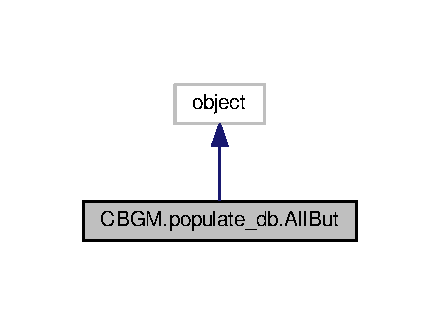
\includegraphics[width=211pt]{classCBGM_1_1populate__db_1_1AllBut__inherit__graph}
\end{center}
\end{figure}


Collaboration diagram for C\+B\+G\+M.\+populate\+\_\+db.\+All\+But\+:\nopagebreak
\begin{figure}[H]
\begin{center}
\leavevmode
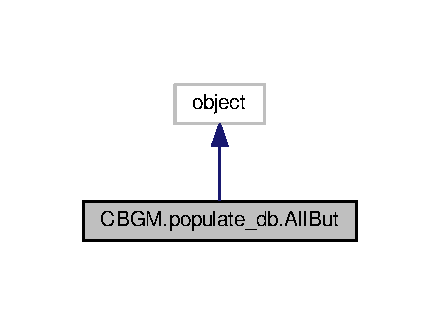
\includegraphics[width=211pt]{classCBGM_1_1populate__db_1_1AllBut__coll__graph}
\end{center}
\end{figure}
\subsection*{Public Member Functions}
\begin{DoxyCompactItemize}
\item 
def \hyperlink{classCBGM_1_1populate__db_1_1AllBut_a7f23c47c62468a12f01159d9fc1f0db5}{\+\_\+\+\_\+init\+\_\+\+\_\+} (self, args)
\item 
def \hyperlink{classCBGM_1_1populate__db_1_1AllBut_a82d4d8c2a8510e574add9123315d8eb9}{calc} (self, all\+\_\+mss)
\end{DoxyCompactItemize}
\subsection*{Public Attributes}
\begin{DoxyCompactItemize}
\item 
\mbox{\Hypertarget{classCBGM_1_1populate__db_1_1AllBut_ae0b181ef4be6024fcb760a638f4b9c91}\label{classCBGM_1_1populate__db_1_1AllBut_ae0b181ef4be6024fcb760a638f4b9c91}} 
{\bfseries args}
\end{DoxyCompactItemize}


\subsection{Constructor \& Destructor Documentation}
\mbox{\Hypertarget{classCBGM_1_1populate__db_1_1AllBut_a7f23c47c62468a12f01159d9fc1f0db5}\label{classCBGM_1_1populate__db_1_1AllBut_a7f23c47c62468a12f01159d9fc1f0db5}} 
\index{C\+B\+G\+M\+::populate\+\_\+db\+::\+All\+But@{C\+B\+G\+M\+::populate\+\_\+db\+::\+All\+But}!\+\_\+\+\_\+init\+\_\+\+\_\+@{\+\_\+\+\_\+init\+\_\+\+\_\+}}
\index{\+\_\+\+\_\+init\+\_\+\+\_\+@{\+\_\+\+\_\+init\+\_\+\+\_\+}!C\+B\+G\+M\+::populate\+\_\+db\+::\+All\+But@{C\+B\+G\+M\+::populate\+\_\+db\+::\+All\+But}}
\subsubsection{\texorpdfstring{\+\_\+\+\_\+init\+\_\+\+\_\+()}{\_\_init\_\_()}}
{\footnotesize\ttfamily def C\+B\+G\+M.\+populate\+\_\+db.\+All\+But.\+\_\+\+\_\+init\+\_\+\+\_\+ (\begin{DoxyParamCaption}\item[{}]{self,  }\item[{}]{args }\end{DoxyParamCaption})}

\begin{DoxyVerb}Class to return a set of all manuscripts minus the ones specified.
\end{DoxyVerb}
 

\subsection{Member Function Documentation}
\mbox{\Hypertarget{classCBGM_1_1populate__db_1_1AllBut_a82d4d8c2a8510e574add9123315d8eb9}\label{classCBGM_1_1populate__db_1_1AllBut_a82d4d8c2a8510e574add9123315d8eb9}} 
\index{C\+B\+G\+M\+::populate\+\_\+db\+::\+All\+But@{C\+B\+G\+M\+::populate\+\_\+db\+::\+All\+But}!calc@{calc}}
\index{calc@{calc}!C\+B\+G\+M\+::populate\+\_\+db\+::\+All\+But@{C\+B\+G\+M\+::populate\+\_\+db\+::\+All\+But}}
\subsubsection{\texorpdfstring{calc()}{calc()}}
{\footnotesize\ttfamily def C\+B\+G\+M.\+populate\+\_\+db.\+All\+But.\+calc (\begin{DoxyParamCaption}\item[{}]{self,  }\item[{}]{all\+\_\+mss }\end{DoxyParamCaption})}

\begin{DoxyVerb}Return a set of all manuscripts minus the ones specified.

@param all_mss: The full list of available manuscripts

Also, 'A' is not included as that's added specially in the __init__ of
class Reading.
\end{DoxyVerb}
 

The documentation for this class was generated from the following file\+:\begin{DoxyCompactItemize}
\item 
populate\+\_\+db.\+py\end{DoxyCompactItemize}

\hypertarget{classanalyse__combinations__of__ancestors_1_1Analyser}{}\section{analyse\+\_\+combinations\+\_\+of\+\_\+ancestors.\+Analyser Class Reference}
\label{classanalyse__combinations__of__ancestors_1_1Analyser}\index{analyse\+\_\+combinations\+\_\+of\+\_\+ancestors.\+Analyser@{analyse\+\_\+combinations\+\_\+of\+\_\+ancestors.\+Analyser}}


Inheritance diagram for analyse\+\_\+combinations\+\_\+of\+\_\+ancestors.\+Analyser\+:\nopagebreak
\begin{figure}[H]
\begin{center}
\leavevmode
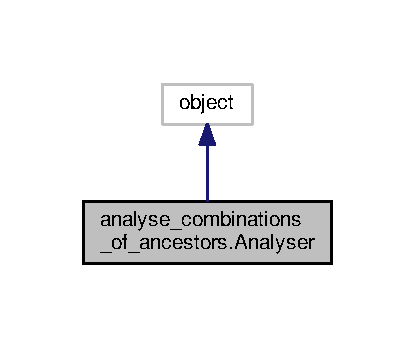
\includegraphics[width=199pt]{classanalyse__combinations__of__ancestors_1_1Analyser__inherit__graph}
\end{center}
\end{figure}


Collaboration diagram for analyse\+\_\+combinations\+\_\+of\+\_\+ancestors.\+Analyser\+:\nopagebreak
\begin{figure}[H]
\begin{center}
\leavevmode
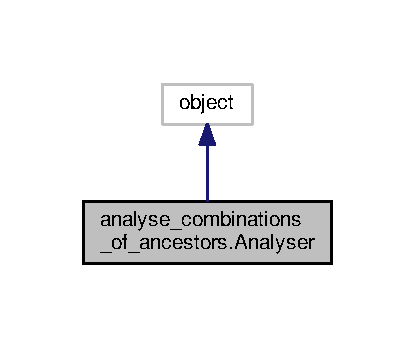
\includegraphics[width=199pt]{classanalyse__combinations__of__ancestors_1_1Analyser__coll__graph}
\end{center}
\end{figure}
\subsection*{Public Member Functions}
\begin{DoxyCompactItemize}
\item 
def \hyperlink{classanalyse__combinations__of__ancestors_1_1Analyser_a877b72ffb4613bf9f2d0f9717433e587}{\+\_\+\+\_\+init\+\_\+\+\_\+} (self, csv\+\_\+file)
\item 
def \hyperlink{classanalyse__combinations__of__ancestors_1_1Analyser_a2bb7870a20c9c9d6d701556b92787059}{analyse} (self, max\+\_\+by\+\_\+posterity=10)
\end{DoxyCompactItemize}
\subsection*{Public Attributes}
\begin{DoxyCompactItemize}
\item 
\mbox{\Hypertarget{classanalyse__combinations__of__ancestors_1_1Analyser_a25fb76f3af03084567625435fa02e435}\label{classanalyse__combinations__of__ancestors_1_1Analyser_a25fb76f3af03084567625435fa02e435}} 
{\bfseries ref}
\item 
\mbox{\Hypertarget{classanalyse__combinations__of__ancestors_1_1Analyser_a160ca764cec07d8aa0e35095b320127d}\label{classanalyse__combinations__of__ancestors_1_1Analyser_a160ca764cec07d8aa0e35095b320127d}} 
{\bfseries has\+\_\+hinweis}
\item 
\mbox{\Hypertarget{classanalyse__combinations__of__ancestors_1_1Analyser_a40c33c0b551a756d038b1a4223d14204}\label{classanalyse__combinations__of__ancestors_1_1Analyser_a40c33c0b551a756d038b1a4223d14204}} 
{\bfseries min\+\_\+offen}
\item 
\mbox{\Hypertarget{classanalyse__combinations__of__ancestors_1_1Analyser_ac36173001c005f16eaad4184bb4686a1}\label{classanalyse__combinations__of__ancestors_1_1Analyser_ac36173001c005f16eaad4184bb4686a1}} 
{\bfseries best\+\_\+rows}
\end{DoxyCompactItemize}


\subsection{Constructor \& Destructor Documentation}
\mbox{\Hypertarget{classanalyse__combinations__of__ancestors_1_1Analyser_a877b72ffb4613bf9f2d0f9717433e587}\label{classanalyse__combinations__of__ancestors_1_1Analyser_a877b72ffb4613bf9f2d0f9717433e587}} 
\index{analyse\+\_\+combinations\+\_\+of\+\_\+ancestors\+::\+Analyser@{analyse\+\_\+combinations\+\_\+of\+\_\+ancestors\+::\+Analyser}!\+\_\+\+\_\+init\+\_\+\+\_\+@{\+\_\+\+\_\+init\+\_\+\+\_\+}}
\index{\+\_\+\+\_\+init\+\_\+\+\_\+@{\+\_\+\+\_\+init\+\_\+\+\_\+}!analyse\+\_\+combinations\+\_\+of\+\_\+ancestors\+::\+Analyser@{analyse\+\_\+combinations\+\_\+of\+\_\+ancestors\+::\+Analyser}}
\subsubsection{\texorpdfstring{\+\_\+\+\_\+init\+\_\+\+\_\+()}{\_\_init\_\_()}}
{\footnotesize\ttfamily def analyse\+\_\+combinations\+\_\+of\+\_\+ancestors.\+Analyser.\+\_\+\+\_\+init\+\_\+\+\_\+ (\begin{DoxyParamCaption}\item[{}]{self,  }\item[{}]{csv\+\_\+file }\end{DoxyParamCaption})}

\begin{DoxyVerb}Load the file, and do simple elimination of unwanted rows
\end{DoxyVerb}
 

\subsection{Member Function Documentation}
\mbox{\Hypertarget{classanalyse__combinations__of__ancestors_1_1Analyser_a2bb7870a20c9c9d6d701556b92787059}\label{classanalyse__combinations__of__ancestors_1_1Analyser_a2bb7870a20c9c9d6d701556b92787059}} 
\index{analyse\+\_\+combinations\+\_\+of\+\_\+ancestors\+::\+Analyser@{analyse\+\_\+combinations\+\_\+of\+\_\+ancestors\+::\+Analyser}!analyse@{analyse}}
\index{analyse@{analyse}!analyse\+\_\+combinations\+\_\+of\+\_\+ancestors\+::\+Analyser@{analyse\+\_\+combinations\+\_\+of\+\_\+ancestors\+::\+Analyser}}
\subsubsection{\texorpdfstring{analyse()}{analyse()}}
{\footnotesize\ttfamily def analyse\+\_\+combinations\+\_\+of\+\_\+ancestors.\+Analyser.\+analyse (\begin{DoxyParamCaption}\item[{}]{self,  }\item[{}]{max\+\_\+by\+\_\+posterity = {\ttfamily 10} }\end{DoxyParamCaption})}

\begin{DoxyVerb}Search for the best row
\end{DoxyVerb}
 

The documentation for this class was generated from the following file\+:\begin{DoxyCompactItemize}
\item 
scripts/analyse\+\_\+combinations\+\_\+of\+\_\+ancestors.\+py\end{DoxyCompactItemize}

\hypertarget{classCBGM_1_1lib_1_1compare__witnesses_1_1Attestations}{}\section{C\+B\+G\+M.\+lib.\+compare\+\_\+witnesses.\+Attestations Class Reference}
\label{classCBGM_1_1lib_1_1compare__witnesses_1_1Attestations}\index{C\+B\+G\+M.\+lib.\+compare\+\_\+witnesses.\+Attestations@{C\+B\+G\+M.\+lib.\+compare\+\_\+witnesses.\+Attestations}}


Inheritance diagram for C\+B\+G\+M.\+lib.\+compare\+\_\+witnesses.\+Attestations\+:\nopagebreak
\begin{figure}[H]
\begin{center}
\leavevmode
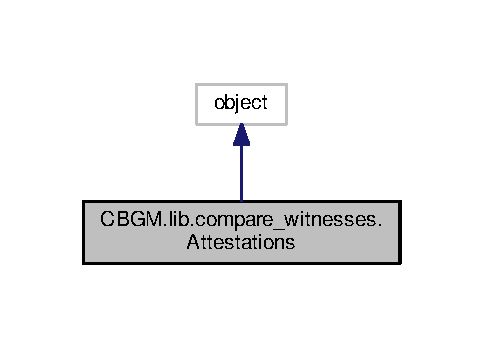
\includegraphics[width=232pt]{classCBGM_1_1lib_1_1compare__witnesses_1_1Attestations__inherit__graph}
\end{center}
\end{figure}


Collaboration diagram for C\+B\+G\+M.\+lib.\+compare\+\_\+witnesses.\+Attestations\+:\nopagebreak
\begin{figure}[H]
\begin{center}
\leavevmode
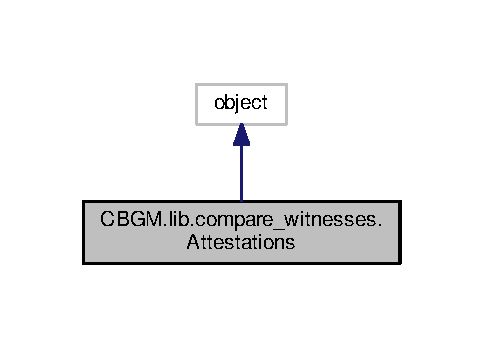
\includegraphics[width=232pt]{classCBGM_1_1lib_1_1compare__witnesses_1_1Attestations__coll__graph}
\end{center}
\end{figure}
\subsection*{Public Member Functions}
\begin{DoxyCompactItemize}
\item 
\mbox{\Hypertarget{classCBGM_1_1lib_1_1compare__witnesses_1_1Attestations_a7f2a79d2f76506e6e5b597bdaf7ca198}\label{classCBGM_1_1lib_1_1compare__witnesses_1_1Attestations_a7f2a79d2f76506e6e5b597bdaf7ca198}} 
def {\bfseries \+\_\+\+\_\+init\+\_\+\+\_\+} (self, db\+\_\+file)
\item 
def \hyperlink{classCBGM_1_1lib_1_1compare__witnesses_1_1Attestations_a98d5c8667a53f75522d2fba7ef19a928}{compare} (self, wits)
\end{DoxyCompactItemize}
\subsection*{Public Attributes}
\begin{DoxyCompactItemize}
\item 
\mbox{\Hypertarget{classCBGM_1_1lib_1_1compare__witnesses_1_1Attestations_ac2a9708ce2afe9a9105b256da6689c15}\label{classCBGM_1_1lib_1_1compare__witnesses_1_1Attestations_ac2a9708ce2afe9a9105b256da6689c15}} 
{\bfseries conn}
\item 
\mbox{\Hypertarget{classCBGM_1_1lib_1_1compare__witnesses_1_1Attestations_a46768ce1b1447a4817a07efdc4372fe0}\label{classCBGM_1_1lib_1_1compare__witnesses_1_1Attestations_a46768ce1b1447a4817a07efdc4372fe0}} 
{\bfseries cursor}
\end{DoxyCompactItemize}


\subsection{Member Function Documentation}
\mbox{\Hypertarget{classCBGM_1_1lib_1_1compare__witnesses_1_1Attestations_a98d5c8667a53f75522d2fba7ef19a928}\label{classCBGM_1_1lib_1_1compare__witnesses_1_1Attestations_a98d5c8667a53f75522d2fba7ef19a928}} 
\index{C\+B\+G\+M\+::lib\+::compare\+\_\+witnesses\+::\+Attestations@{C\+B\+G\+M\+::lib\+::compare\+\_\+witnesses\+::\+Attestations}!compare@{compare}}
\index{compare@{compare}!C\+B\+G\+M\+::lib\+::compare\+\_\+witnesses\+::\+Attestations@{C\+B\+G\+M\+::lib\+::compare\+\_\+witnesses\+::\+Attestations}}
\subsubsection{\texorpdfstring{compare()}{compare()}}
{\footnotesize\ttfamily def C\+B\+G\+M.\+lib.\+compare\+\_\+witnesses.\+Attestations.\+compare (\begin{DoxyParamCaption}\item[{}]{self,  }\item[{}]{wits }\end{DoxyParamCaption})}

\begin{DoxyVerb}Compare the attestations of the supplied pair of witnesses, showing where they agree and what relationship
they have where they disagree (if any).
:param wits: list of witness names
:return: (string) report
\end{DoxyVerb}
 

The documentation for this class was generated from the following file\+:\begin{DoxyCompactItemize}
\item 
lib/compare\+\_\+witnesses.\+py\end{DoxyCompactItemize}

\hypertarget{classCBGM_1_1check__consistency_1_1CheckConsistency}{}\section{C\+B\+G\+M.\+check\+\_\+consistency.\+Check\+Consistency Class Reference}
\label{classCBGM_1_1check__consistency_1_1CheckConsistency}\index{C\+B\+G\+M.\+check\+\_\+consistency.\+Check\+Consistency@{C\+B\+G\+M.\+check\+\_\+consistency.\+Check\+Consistency}}


Inheritance diagram for C\+B\+G\+M.\+check\+\_\+consistency.\+Check\+Consistency\+:\nopagebreak
\begin{figure}[H]
\begin{center}
\leavevmode
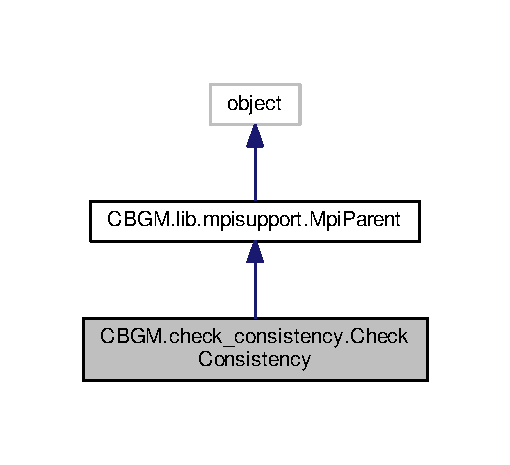
\includegraphics[width=245pt]{classCBGM_1_1check__consistency_1_1CheckConsistency__inherit__graph}
\end{center}
\end{figure}


Collaboration diagram for C\+B\+G\+M.\+check\+\_\+consistency.\+Check\+Consistency\+:\nopagebreak
\begin{figure}[H]
\begin{center}
\leavevmode
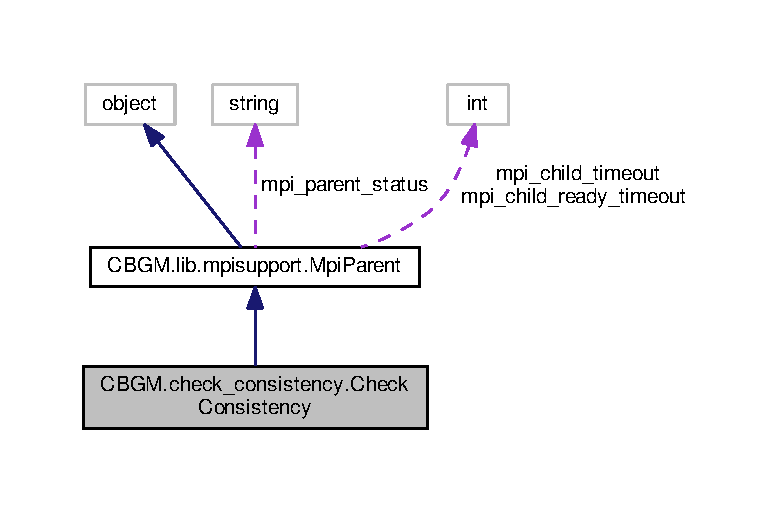
\includegraphics[width=350pt]{classCBGM_1_1check__consistency_1_1CheckConsistency__coll__graph}
\end{center}
\end{figure}
\subsection*{Public Member Functions}
\begin{DoxyCompactItemize}
\item 
\mbox{\Hypertarget{classCBGM_1_1check__consistency_1_1CheckConsistency_a3d8ee224f2ab9fd798c357dc8b63274c}\label{classCBGM_1_1check__consistency_1_1CheckConsistency_a3d8ee224f2ab9fd798c357dc8b63274c}} 
def {\bfseries \+\_\+\+\_\+init\+\_\+\+\_\+} (self, inputfile, connectivity)
\item 
def \hyperlink{classCBGM_1_1check__consistency_1_1CheckConsistency_a7f800c25db68d0c3af20fdd478eb749d}{collate\+\_\+results} (self)
\item 
def \hyperlink{classCBGM_1_1check__consistency_1_1CheckConsistency_a7264e4aabf713a19c984a4da92fa42fb}{mpi\+\_\+handle\+\_\+result} (self, args, ret)
\end{DoxyCompactItemize}
\subsection*{Public Attributes}
\begin{DoxyCompactItemize}
\item 
\mbox{\Hypertarget{classCBGM_1_1check__consistency_1_1CheckConsistency_a08b4e42b36509e0450d17db4373315cb}\label{classCBGM_1_1check__consistency_1_1CheckConsistency_a08b4e42b36509e0450d17db4373315cb}} 
{\bfseries results}
\item 
\mbox{\Hypertarget{classCBGM_1_1check__consistency_1_1CheckConsistency_a9431c811d6487d192b80e61101629020}\label{classCBGM_1_1check__consistency_1_1CheckConsistency_a9431c811d6487d192b80e61101629020}} 
{\bfseries connectivity}
\item 
\mbox{\Hypertarget{classCBGM_1_1check__consistency_1_1CheckConsistency_acb5baa0394ce9e10063dab362367420c}\label{classCBGM_1_1check__consistency_1_1CheckConsistency_acb5baa0394ce9e10063dab362367420c}} 
{\bfseries working\+\_\+dir}
\item 
\mbox{\Hypertarget{classCBGM_1_1check__consistency_1_1CheckConsistency_a3090b324b6d7b2dc2c079bdfe93e7651}\label{classCBGM_1_1check__consistency_1_1CheckConsistency_a3090b324b6d7b2dc2c079bdfe93e7651}} 
{\bfseries vus}
\end{DoxyCompactItemize}
\subsection*{Additional Inherited Members}


\subsection{Member Function Documentation}
\mbox{\Hypertarget{classCBGM_1_1check__consistency_1_1CheckConsistency_a7f800c25db68d0c3af20fdd478eb749d}\label{classCBGM_1_1check__consistency_1_1CheckConsistency_a7f800c25db68d0c3af20fdd478eb749d}} 
\index{C\+B\+G\+M\+::check\+\_\+consistency\+::\+Check\+Consistency@{C\+B\+G\+M\+::check\+\_\+consistency\+::\+Check\+Consistency}!collate\+\_\+results@{collate\+\_\+results}}
\index{collate\+\_\+results@{collate\+\_\+results}!C\+B\+G\+M\+::check\+\_\+consistency\+::\+Check\+Consistency@{C\+B\+G\+M\+::check\+\_\+consistency\+::\+Check\+Consistency}}
\subsubsection{\texorpdfstring{collate\+\_\+results()}{collate\_results()}}
{\footnotesize\ttfamily def C\+B\+G\+M.\+check\+\_\+consistency.\+Check\+Consistency.\+collate\+\_\+results (\begin{DoxyParamCaption}\item[{}]{self }\end{DoxyParamCaption})}

\begin{DoxyVerb}Write the HTML file
\end{DoxyVerb}
 \mbox{\Hypertarget{classCBGM_1_1check__consistency_1_1CheckConsistency_a7264e4aabf713a19c984a4da92fa42fb}\label{classCBGM_1_1check__consistency_1_1CheckConsistency_a7264e4aabf713a19c984a4da92fa42fb}} 
\index{C\+B\+G\+M\+::check\+\_\+consistency\+::\+Check\+Consistency@{C\+B\+G\+M\+::check\+\_\+consistency\+::\+Check\+Consistency}!mpi\+\_\+handle\+\_\+result@{mpi\+\_\+handle\+\_\+result}}
\index{mpi\+\_\+handle\+\_\+result@{mpi\+\_\+handle\+\_\+result}!C\+B\+G\+M\+::check\+\_\+consistency\+::\+Check\+Consistency@{C\+B\+G\+M\+::check\+\_\+consistency\+::\+Check\+Consistency}}
\subsubsection{\texorpdfstring{mpi\+\_\+handle\+\_\+result()}{mpi\_handle\_result()}}
{\footnotesize\ttfamily def C\+B\+G\+M.\+check\+\_\+consistency.\+Check\+Consistency.\+mpi\+\_\+handle\+\_\+result (\begin{DoxyParamCaption}\item[{}]{self,  }\item[{}]{args,  }\item[{}]{ret }\end{DoxyParamCaption})}

\begin{DoxyVerb}Handle an MPI result
@param args: original args sent to the child
@param ret: response from the child
\end{DoxyVerb}
 

The documentation for this class was generated from the following file\+:\begin{DoxyCompactItemize}
\item 
check\+\_\+consistency.\+py\end{DoxyCompactItemize}

\hypertarget{classCBGM_1_1lib_1_1pre__genealogical__coherence_1_1Coherence}{}\section{C\+B\+G\+M.\+lib.\+pre\+\_\+genealogical\+\_\+coherence.\+Coherence Class Reference}
\label{classCBGM_1_1lib_1_1pre__genealogical__coherence_1_1Coherence}\index{C\+B\+G\+M.\+lib.\+pre\+\_\+genealogical\+\_\+coherence.\+Coherence@{C\+B\+G\+M.\+lib.\+pre\+\_\+genealogical\+\_\+coherence.\+Coherence}}


Inheritance diagram for C\+B\+G\+M.\+lib.\+pre\+\_\+genealogical\+\_\+coherence.\+Coherence\+:\nopagebreak
\begin{figure}[H]
\begin{center}
\leavevmode
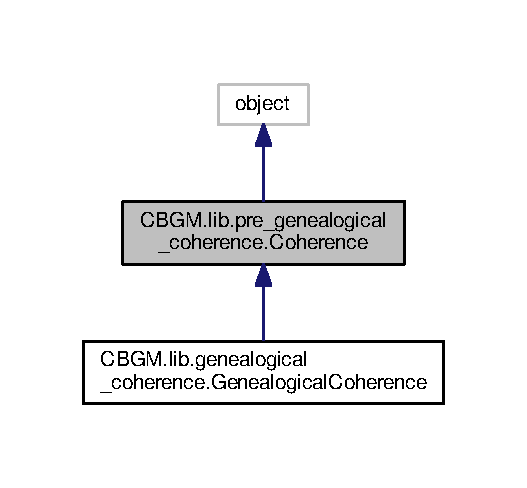
\includegraphics[width=253pt]{classCBGM_1_1lib_1_1pre__genealogical__coherence_1_1Coherence__inherit__graph}
\end{center}
\end{figure}


Collaboration diagram for C\+B\+G\+M.\+lib.\+pre\+\_\+genealogical\+\_\+coherence.\+Coherence\+:\nopagebreak
\begin{figure}[H]
\begin{center}
\leavevmode
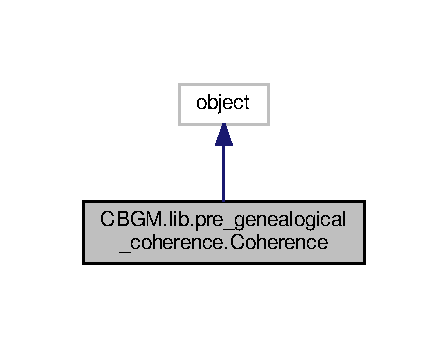
\includegraphics[width=215pt]{classCBGM_1_1lib_1_1pre__genealogical__coherence_1_1Coherence__coll__graph}
\end{center}
\end{figure}
\subsection*{Public Member Functions}
\begin{DoxyCompactItemize}
\item 
def \hyperlink{classCBGM_1_1lib_1_1pre__genealogical__coherence_1_1Coherence_ae6841155c04b8c5dcf22279b008cb96e}{\+\_\+\+\_\+init\+\_\+\+\_\+} (self, db\+\_\+file, w1, pretty\+\_\+p=True, debug=False, use\+\_\+cache=False)
\item 
def \hyperlink{classCBGM_1_1lib_1_1pre__genealogical__coherence_1_1Coherence_af601453fe8d3cd09f1aff40cab2eb337}{set\+\_\+variant\+\_\+unit} (self, variant\+\_\+unit)
\item 
def \hyperlink{classCBGM_1_1lib_1_1pre__genealogical__coherence_1_1Coherence_a08998731ef4735695399d884926caa1f}{generate} (self)
\item 
def \hyperlink{classCBGM_1_1lib_1_1pre__genealogical__coherence_1_1Coherence_a3cce8769d2fb90b5290231dc8fffb949}{all\+\_\+attestations} (self)
\item 
def \hyperlink{classCBGM_1_1lib_1_1pre__genealogical__coherence_1_1Coherence_a3e7881f5c9a2e7c2762c4d747bf0f4f5}{get\+\_\+attestation} (self, witness, vu)
\item 
def \hyperlink{classCBGM_1_1lib_1_1pre__genealogical__coherence_1_1Coherence_a977c8850361d5d9cf60d0098cdc0e4a7}{tab\+\_\+delim\+\_\+table} (self)
\end{DoxyCompactItemize}
\subsection*{Public Attributes}
\begin{DoxyCompactItemize}
\item 
\mbox{\Hypertarget{classCBGM_1_1lib_1_1pre__genealogical__coherence_1_1Coherence_a69f5906051d8671424c7846b82fd4d13}\label{classCBGM_1_1lib_1_1pre__genealogical__coherence_1_1Coherence_a69f5906051d8671424c7846b82fd4d13}} 
{\bfseries conn}
\item 
\mbox{\Hypertarget{classCBGM_1_1lib_1_1pre__genealogical__coherence_1_1Coherence_ad820fddbd9452f5dc0eccf6dde855126}\label{classCBGM_1_1lib_1_1pre__genealogical__coherence_1_1Coherence_ad820fddbd9452f5dc0eccf6dde855126}} 
{\bfseries cursor}
\item 
\mbox{\Hypertarget{classCBGM_1_1lib_1_1pre__genealogical__coherence_1_1Coherence_add2cdb3bfcf9b1a2dc8b706a482e9549}\label{classCBGM_1_1lib_1_1pre__genealogical__coherence_1_1Coherence_add2cdb3bfcf9b1a2dc8b706a482e9549}} 
{\bfseries w1}
\item 
\mbox{\Hypertarget{classCBGM_1_1lib_1_1pre__genealogical__coherence_1_1Coherence_ae575c9704d0cea692deb44ae9a1c11e0}\label{classCBGM_1_1lib_1_1pre__genealogical__coherence_1_1Coherence_ae575c9704d0cea692deb44ae9a1c11e0}} 
{\bfseries rows}
\item 
\mbox{\Hypertarget{classCBGM_1_1lib_1_1pre__genealogical__coherence_1_1Coherence_a948f87808ae1488617177fc78e9ab365}\label{classCBGM_1_1lib_1_1pre__genealogical__coherence_1_1Coherence_a948f87808ae1488617177fc78e9ab365}} 
{\bfseries columns}
\item 
\mbox{\Hypertarget{classCBGM_1_1lib_1_1pre__genealogical__coherence_1_1Coherence_ae97cbc8c5bf5b8a0107cfdbedf0dd226}\label{classCBGM_1_1lib_1_1pre__genealogical__coherence_1_1Coherence_ae97cbc8c5bf5b8a0107cfdbedf0dd226}} 
{\bfseries pretty\+\_\+p}
\item 
\mbox{\Hypertarget{classCBGM_1_1lib_1_1pre__genealogical__coherence_1_1Coherence_a1ad8ac5a0f35f920f1514c2989c369f5}\label{classCBGM_1_1lib_1_1pre__genealogical__coherence_1_1Coherence_a1ad8ac5a0f35f920f1514c2989c369f5}} 
{\bfseries debug}
\item 
\mbox{\Hypertarget{classCBGM_1_1lib_1_1pre__genealogical__coherence_1_1Coherence_a13944fe90892312717c1c246a40cd031}\label{classCBGM_1_1lib_1_1pre__genealogical__coherence_1_1Coherence_a13944fe90892312717c1c246a40cd031}} 
{\bfseries variant\+\_\+unit}
\item 
\mbox{\Hypertarget{classCBGM_1_1lib_1_1pre__genealogical__coherence_1_1Coherence_a4edf96f162a45b4af585a082c7c07d64}\label{classCBGM_1_1lib_1_1pre__genealogical__coherence_1_1Coherence_a4edf96f162a45b4af585a082c7c07d64}} 
{\bfseries use\+\_\+cache}
\item 
\mbox{\Hypertarget{classCBGM_1_1lib_1_1pre__genealogical__coherence_1_1Coherence_a552d93c81345c3554b6b71de9d1725bb}\label{classCBGM_1_1lib_1_1pre__genealogical__coherence_1_1Coherence_a552d93c81345c3554b6b71de9d1725bb}} 
{\bfseries formatters}
\item 
\mbox{\Hypertarget{classCBGM_1_1lib_1_1pre__genealogical__coherence_1_1Coherence_ad8e23b28e8768d1ea071d4718e8bad59}\label{classCBGM_1_1lib_1_1pre__genealogical__coherence_1_1Coherence_ad8e23b28e8768d1ea071d4718e8bad59}} 
{\bfseries all\+\_\+mss}
\end{DoxyCompactItemize}


\subsection{Detailed Description}
\begin{DoxyVerb}Class representing pre-genealogical coherence that can be extended
to give more info.
\end{DoxyVerb}
 

\subsection{Constructor \& Destructor Documentation}
\mbox{\Hypertarget{classCBGM_1_1lib_1_1pre__genealogical__coherence_1_1Coherence_ae6841155c04b8c5dcf22279b008cb96e}\label{classCBGM_1_1lib_1_1pre__genealogical__coherence_1_1Coherence_ae6841155c04b8c5dcf22279b008cb96e}} 
\index{C\+B\+G\+M\+::lib\+::pre\+\_\+genealogical\+\_\+coherence\+::\+Coherence@{C\+B\+G\+M\+::lib\+::pre\+\_\+genealogical\+\_\+coherence\+::\+Coherence}!\+\_\+\+\_\+init\+\_\+\+\_\+@{\+\_\+\+\_\+init\+\_\+\+\_\+}}
\index{\+\_\+\+\_\+init\+\_\+\+\_\+@{\+\_\+\+\_\+init\+\_\+\+\_\+}!C\+B\+G\+M\+::lib\+::pre\+\_\+genealogical\+\_\+coherence\+::\+Coherence@{C\+B\+G\+M\+::lib\+::pre\+\_\+genealogical\+\_\+coherence\+::\+Coherence}}
\subsubsection{\texorpdfstring{\+\_\+\+\_\+init\+\_\+\+\_\+()}{\_\_init\_\_()}}
{\footnotesize\ttfamily def C\+B\+G\+M.\+lib.\+pre\+\_\+genealogical\+\_\+coherence.\+Coherence.\+\_\+\+\_\+init\+\_\+\+\_\+ (\begin{DoxyParamCaption}\item[{}]{self,  }\item[{}]{db\+\_\+file,  }\item[{}]{w1,  }\item[{}]{pretty\+\_\+p = {\ttfamily True},  }\item[{}]{debug = {\ttfamily False},  }\item[{}]{use\+\_\+cache = {\ttfamily False} }\end{DoxyParamCaption})}

\begin{DoxyVerb}@param db_file: database file
@param w1: witness 1 name
@param pretty_p: normal P or the gothic (pretty) one
@param debug: show more columns for debugging
@param use_cache: use the file cache for this db to speed things up
\end{DoxyVerb}
 

\subsection{Member Function Documentation}
\mbox{\Hypertarget{classCBGM_1_1lib_1_1pre__genealogical__coherence_1_1Coherence_a3cce8769d2fb90b5290231dc8fffb949}\label{classCBGM_1_1lib_1_1pre__genealogical__coherence_1_1Coherence_a3cce8769d2fb90b5290231dc8fffb949}} 
\index{C\+B\+G\+M\+::lib\+::pre\+\_\+genealogical\+\_\+coherence\+::\+Coherence@{C\+B\+G\+M\+::lib\+::pre\+\_\+genealogical\+\_\+coherence\+::\+Coherence}!all\+\_\+attestations@{all\+\_\+attestations}}
\index{all\+\_\+attestations@{all\+\_\+attestations}!C\+B\+G\+M\+::lib\+::pre\+\_\+genealogical\+\_\+coherence\+::\+Coherence@{C\+B\+G\+M\+::lib\+::pre\+\_\+genealogical\+\_\+coherence\+::\+Coherence}}
\subsubsection{\texorpdfstring{all\+\_\+attestations()}{all\_attestations()}}
{\footnotesize\ttfamily def C\+B\+G\+M.\+lib.\+pre\+\_\+genealogical\+\_\+coherence.\+Coherence.\+all\+\_\+attestations (\begin{DoxyParamCaption}\item[{}]{self }\end{DoxyParamCaption})}

\begin{DoxyVerb}All attestations - getting this piecemeal is slow, so we'll cache it
\end{DoxyVerb}
 \mbox{\Hypertarget{classCBGM_1_1lib_1_1pre__genealogical__coherence_1_1Coherence_a08998731ef4735695399d884926caa1f}\label{classCBGM_1_1lib_1_1pre__genealogical__coherence_1_1Coherence_a08998731ef4735695399d884926caa1f}} 
\index{C\+B\+G\+M\+::lib\+::pre\+\_\+genealogical\+\_\+coherence\+::\+Coherence@{C\+B\+G\+M\+::lib\+::pre\+\_\+genealogical\+\_\+coherence\+::\+Coherence}!generate@{generate}}
\index{generate@{generate}!C\+B\+G\+M\+::lib\+::pre\+\_\+genealogical\+\_\+coherence\+::\+Coherence@{C\+B\+G\+M\+::lib\+::pre\+\_\+genealogical\+\_\+coherence\+::\+Coherence}}
\subsubsection{\texorpdfstring{generate()}{generate()}}
{\footnotesize\ttfamily def C\+B\+G\+M.\+lib.\+pre\+\_\+genealogical\+\_\+coherence.\+Coherence.\+generate (\begin{DoxyParamCaption}\item[{}]{self }\end{DoxyParamCaption})}

\begin{DoxyVerb}Generate the data
\end{DoxyVerb}
 \mbox{\Hypertarget{classCBGM_1_1lib_1_1pre__genealogical__coherence_1_1Coherence_a3e7881f5c9a2e7c2762c4d747bf0f4f5}\label{classCBGM_1_1lib_1_1pre__genealogical__coherence_1_1Coherence_a3e7881f5c9a2e7c2762c4d747bf0f4f5}} 
\index{C\+B\+G\+M\+::lib\+::pre\+\_\+genealogical\+\_\+coherence\+::\+Coherence@{C\+B\+G\+M\+::lib\+::pre\+\_\+genealogical\+\_\+coherence\+::\+Coherence}!get\+\_\+attestation@{get\+\_\+attestation}}
\index{get\+\_\+attestation@{get\+\_\+attestation}!C\+B\+G\+M\+::lib\+::pre\+\_\+genealogical\+\_\+coherence\+::\+Coherence@{C\+B\+G\+M\+::lib\+::pre\+\_\+genealogical\+\_\+coherence\+::\+Coherence}}
\subsubsection{\texorpdfstring{get\+\_\+attestation()}{get\_attestation()}}
{\footnotesize\ttfamily def C\+B\+G\+M.\+lib.\+pre\+\_\+genealogical\+\_\+coherence.\+Coherence.\+get\+\_\+attestation (\begin{DoxyParamCaption}\item[{}]{self,  }\item[{}]{witness,  }\item[{}]{vu }\end{DoxyParamCaption})}

\begin{DoxyVerb}A cache to find out what a witness reads in a variant unit
\end{DoxyVerb}
 \mbox{\Hypertarget{classCBGM_1_1lib_1_1pre__genealogical__coherence_1_1Coherence_af601453fe8d3cd09f1aff40cab2eb337}\label{classCBGM_1_1lib_1_1pre__genealogical__coherence_1_1Coherence_af601453fe8d3cd09f1aff40cab2eb337}} 
\index{C\+B\+G\+M\+::lib\+::pre\+\_\+genealogical\+\_\+coherence\+::\+Coherence@{C\+B\+G\+M\+::lib\+::pre\+\_\+genealogical\+\_\+coherence\+::\+Coherence}!set\+\_\+variant\+\_\+unit@{set\+\_\+variant\+\_\+unit}}
\index{set\+\_\+variant\+\_\+unit@{set\+\_\+variant\+\_\+unit}!C\+B\+G\+M\+::lib\+::pre\+\_\+genealogical\+\_\+coherence\+::\+Coherence@{C\+B\+G\+M\+::lib\+::pre\+\_\+genealogical\+\_\+coherence\+::\+Coherence}}
\subsubsection{\texorpdfstring{set\+\_\+variant\+\_\+unit()}{set\_variant\_unit()}}
{\footnotesize\ttfamily def C\+B\+G\+M.\+lib.\+pre\+\_\+genealogical\+\_\+coherence.\+Coherence.\+set\+\_\+variant\+\_\+unit (\begin{DoxyParamCaption}\item[{}]{self,  }\item[{}]{variant\+\_\+unit }\end{DoxyParamCaption})}

\begin{DoxyVerb}Specify a non-None variant unit to extend the data in this coherence object.

We use this extra method (rather than the constructor) since the coherence data can be cached without the
variant unit and used later for other variant units.

This adds extra data to existing rows, if they've been generated.
\end{DoxyVerb}
 \mbox{\Hypertarget{classCBGM_1_1lib_1_1pre__genealogical__coherence_1_1Coherence_a977c8850361d5d9cf60d0098cdc0e4a7}\label{classCBGM_1_1lib_1_1pre__genealogical__coherence_1_1Coherence_a977c8850361d5d9cf60d0098cdc0e4a7}} 
\index{C\+B\+G\+M\+::lib\+::pre\+\_\+genealogical\+\_\+coherence\+::\+Coherence@{C\+B\+G\+M\+::lib\+::pre\+\_\+genealogical\+\_\+coherence\+::\+Coherence}!tab\+\_\+delim\+\_\+table@{tab\+\_\+delim\+\_\+table}}
\index{tab\+\_\+delim\+\_\+table@{tab\+\_\+delim\+\_\+table}!C\+B\+G\+M\+::lib\+::pre\+\_\+genealogical\+\_\+coherence\+::\+Coherence@{C\+B\+G\+M\+::lib\+::pre\+\_\+genealogical\+\_\+coherence\+::\+Coherence}}
\subsubsection{\texorpdfstring{tab\+\_\+delim\+\_\+table()}{tab\_delim\_table()}}
{\footnotesize\ttfamily def C\+B\+G\+M.\+lib.\+pre\+\_\+genealogical\+\_\+coherence.\+Coherence.\+tab\+\_\+delim\+\_\+table (\begin{DoxyParamCaption}\item[{}]{self }\end{DoxyParamCaption})}

\begin{DoxyVerb}Returns a tab delimited table of the data
\end{DoxyVerb}
 

The documentation for this class was generated from the following file\+:\begin{DoxyCompactItemize}
\item 
lib/pre\+\_\+genealogical\+\_\+coherence.\+py\end{DoxyCompactItemize}

\hypertarget{classCBGM_1_1lib_1_1genealogical__coherence_1_1CyclicDependency}{}\section{C\+B\+G\+M.\+lib.\+genealogical\+\_\+coherence.\+Cyclic\+Dependency Class Reference}
\label{classCBGM_1_1lib_1_1genealogical__coherence_1_1CyclicDependency}\index{C\+B\+G\+M.\+lib.\+genealogical\+\_\+coherence.\+Cyclic\+Dependency@{C\+B\+G\+M.\+lib.\+genealogical\+\_\+coherence.\+Cyclic\+Dependency}}


Inheritance diagram for C\+B\+G\+M.\+lib.\+genealogical\+\_\+coherence.\+Cyclic\+Dependency\+:\nopagebreak
\begin{figure}[H]
\begin{center}
\leavevmode
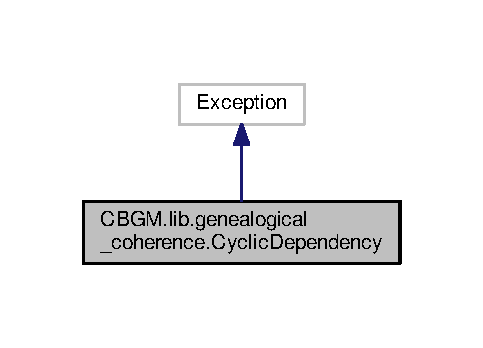
\includegraphics[width=232pt]{classCBGM_1_1lib_1_1genealogical__coherence_1_1CyclicDependency__inherit__graph}
\end{center}
\end{figure}


Collaboration diagram for C\+B\+G\+M.\+lib.\+genealogical\+\_\+coherence.\+Cyclic\+Dependency\+:\nopagebreak
\begin{figure}[H]
\begin{center}
\leavevmode
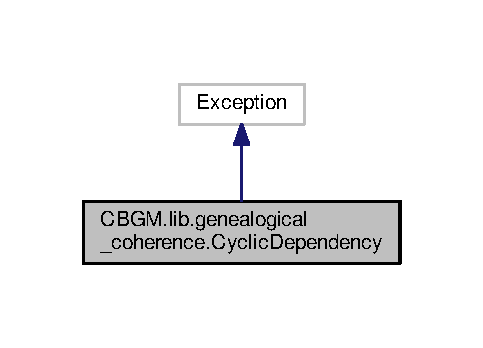
\includegraphics[width=232pt]{classCBGM_1_1lib_1_1genealogical__coherence_1_1CyclicDependency__coll__graph}
\end{center}
\end{figure}


The documentation for this class was generated from the following file\+:\begin{DoxyCompactItemize}
\item 
lib/genealogical\+\_\+coherence.\+py\end{DoxyCompactItemize}

\hypertarget{classCBGM_1_1lib_1_1textual__flow_1_1ForestError}{}\section{C\+B\+G\+M.\+lib.\+textual\+\_\+flow.\+Forest\+Error Class Reference}
\label{classCBGM_1_1lib_1_1textual__flow_1_1ForestError}\index{C\+B\+G\+M.\+lib.\+textual\+\_\+flow.\+Forest\+Error@{C\+B\+G\+M.\+lib.\+textual\+\_\+flow.\+Forest\+Error}}


Inheritance diagram for C\+B\+G\+M.\+lib.\+textual\+\_\+flow.\+Forest\+Error\+:\nopagebreak
\begin{figure}[H]
\begin{center}
\leavevmode
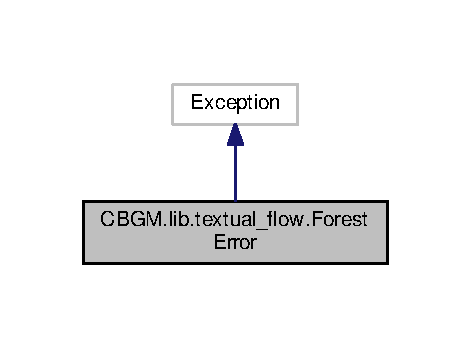
\includegraphics[width=226pt]{classCBGM_1_1lib_1_1textual__flow_1_1ForestError__inherit__graph}
\end{center}
\end{figure}


Collaboration diagram for C\+B\+G\+M.\+lib.\+textual\+\_\+flow.\+Forest\+Error\+:\nopagebreak
\begin{figure}[H]
\begin{center}
\leavevmode
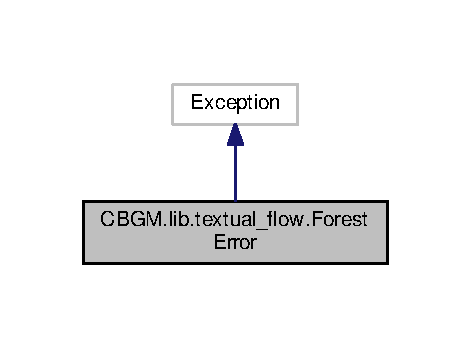
\includegraphics[width=226pt]{classCBGM_1_1lib_1_1textual__flow_1_1ForestError__coll__graph}
\end{center}
\end{figure}


The documentation for this class was generated from the following file\+:\begin{DoxyCompactItemize}
\item 
lib/textual\+\_\+flow.\+py\end{DoxyCompactItemize}

\hypertarget{classCBGM_1_1lib_1_1genealogical__coherence_1_1GenealogicalCoherence}{}\section{C\+B\+G\+M.\+lib.\+genealogical\+\_\+coherence.\+Genealogical\+Coherence Class Reference}
\label{classCBGM_1_1lib_1_1genealogical__coherence_1_1GenealogicalCoherence}\index{C\+B\+G\+M.\+lib.\+genealogical\+\_\+coherence.\+Genealogical\+Coherence@{C\+B\+G\+M.\+lib.\+genealogical\+\_\+coherence.\+Genealogical\+Coherence}}


Inheritance diagram for C\+B\+G\+M.\+lib.\+genealogical\+\_\+coherence.\+Genealogical\+Coherence\+:\nopagebreak
\begin{figure}[H]
\begin{center}
\leavevmode
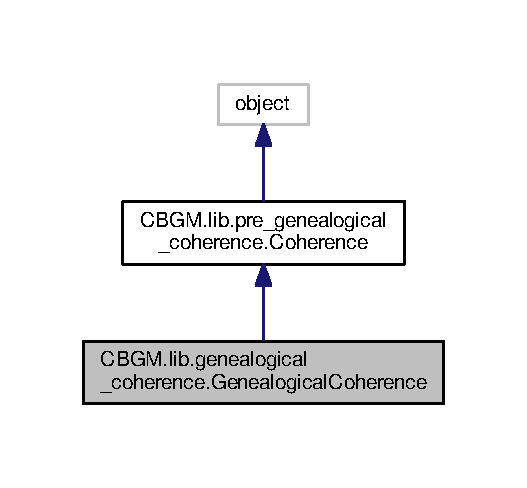
\includegraphics[width=253pt]{classCBGM_1_1lib_1_1genealogical__coherence_1_1GenealogicalCoherence__inherit__graph}
\end{center}
\end{figure}


Collaboration diagram for C\+B\+G\+M.\+lib.\+genealogical\+\_\+coherence.\+Genealogical\+Coherence\+:\nopagebreak
\begin{figure}[H]
\begin{center}
\leavevmode
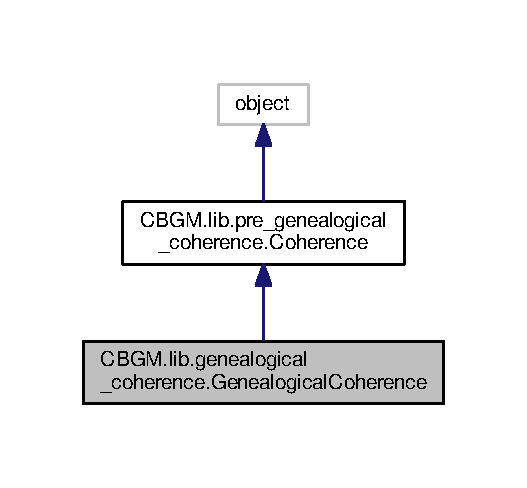
\includegraphics[width=253pt]{classCBGM_1_1lib_1_1genealogical__coherence_1_1GenealogicalCoherence__coll__graph}
\end{center}
\end{figure}
\subsection*{Public Member Functions}
\begin{DoxyCompactItemize}
\item 
\mbox{\Hypertarget{classCBGM_1_1lib_1_1genealogical__coherence_1_1GenealogicalCoherence_a97d498f36897e5bcfd3f1d8821358642}\label{classCBGM_1_1lib_1_1genealogical__coherence_1_1GenealogicalCoherence_a97d498f36897e5bcfd3f1d8821358642}} 
def {\bfseries \+\_\+\+\_\+init\+\_\+\+\_\+} (self, o, min\+\_\+strength=None, k)
\item 
def \hyperlink{classCBGM_1_1lib_1_1genealogical__coherence_1_1GenealogicalCoherence_a85db3f16efe9e55e34d2d6f22d9abfe9}{generate} (self)
\item 
def \hyperlink{classCBGM_1_1lib_1_1genealogical__coherence_1_1GenealogicalCoherence_af457b8df3b3ff1dbd846114e352f6715}{add\+\_\+D} (self, w2, row)
\item 
def \hyperlink{classCBGM_1_1lib_1_1genealogical__coherence_1_1GenealogicalCoherence_adb225962d134e23024f5072994ea9d73}{add\+\_\+\+W1\+\_\+lt\+\_\+\+W2} (self, w2, row)
\item 
def \hyperlink{classCBGM_1_1lib_1_1genealogical__coherence_1_1GenealogicalCoherence_a21319e40e3e74f13c007f49d71468d07}{add\+\_\+\+W1\+\_\+gt\+\_\+\+W2} (self, w2, row)
\item 
def \hyperlink{classCBGM_1_1lib_1_1genealogical__coherence_1_1GenealogicalCoherence_ab190887d1943928f03642eba77928bc4}{add\+\_\+\+U\+N\+CL} (self, w2, row)
\item 
def \hyperlink{classCBGM_1_1lib_1_1genealogical__coherence_1_1GenealogicalCoherence_a78b9d863a9d1db1cdb483bc62172198d}{add\+\_\+\+N\+O\+R\+EL} (self, w2, row)
\item 
def \hyperlink{classCBGM_1_1lib_1_1genealogical__coherence_1_1GenealogicalCoherence_af1572e7d21def128aaacac243d3ec348}{potential\+\_\+ancestors} (self)
\item 
def \hyperlink{classCBGM_1_1lib_1_1genealogical__coherence_1_1GenealogicalCoherence_aad49647f1473cb8aca60c1792a046b7b}{parent\+\_\+combinations} (self, reading, parent\+\_\+reading, max\+\_\+rank=None, min\+\_\+perc=None, include\+\_\+undirected=False, my\+\_\+gen=1)
\end{DoxyCompactItemize}
\subsection*{Public Attributes}
\begin{DoxyCompactItemize}
\item 
\mbox{\Hypertarget{classCBGM_1_1lib_1_1genealogical__coherence_1_1GenealogicalCoherence_a73556ba9b0c96280652dda16885f62d9}\label{classCBGM_1_1lib_1_1genealogical__coherence_1_1GenealogicalCoherence_a73556ba9b0c96280652dda16885f62d9}} 
{\bfseries reading\+\_\+relationships}
\item 
\mbox{\Hypertarget{classCBGM_1_1lib_1_1genealogical__coherence_1_1GenealogicalCoherence_a552a14d4dab619fc94baeda2ac6929a5}\label{classCBGM_1_1lib_1_1genealogical__coherence_1_1GenealogicalCoherence_a552a14d4dab619fc94baeda2ac6929a5}} 
{\bfseries min\+\_\+strength}
\item 
\mbox{\Hypertarget{classCBGM_1_1lib_1_1genealogical__coherence_1_1GenealogicalCoherence_aa94934fe6d1678d1f818e27e4a654b39}\label{classCBGM_1_1lib_1_1genealogical__coherence_1_1GenealogicalCoherence_aa94934fe6d1678d1f818e27e4a654b39}} 
{\bfseries rows}
\end{DoxyCompactItemize}


\subsection{Detailed Description}
\begin{DoxyVerb}Class representing genealogical coherence (potential ancestors)
\end{DoxyVerb}
 

\subsection{Member Function Documentation}
\mbox{\Hypertarget{classCBGM_1_1lib_1_1genealogical__coherence_1_1GenealogicalCoherence_af457b8df3b3ff1dbd846114e352f6715}\label{classCBGM_1_1lib_1_1genealogical__coherence_1_1GenealogicalCoherence_af457b8df3b3ff1dbd846114e352f6715}} 
\index{C\+B\+G\+M\+::lib\+::genealogical\+\_\+coherence\+::\+Genealogical\+Coherence@{C\+B\+G\+M\+::lib\+::genealogical\+\_\+coherence\+::\+Genealogical\+Coherence}!add\+\_\+D@{add\+\_\+D}}
\index{add\+\_\+D@{add\+\_\+D}!C\+B\+G\+M\+::lib\+::genealogical\+\_\+coherence\+::\+Genealogical\+Coherence@{C\+B\+G\+M\+::lib\+::genealogical\+\_\+coherence\+::\+Genealogical\+Coherence}}
\subsubsection{\texorpdfstring{add\+\_\+\+D()}{add\_D()}}
{\footnotesize\ttfamily def C\+B\+G\+M.\+lib.\+genealogical\+\_\+coherence.\+Genealogical\+Coherence.\+add\+\_\+D (\begin{DoxyParamCaption}\item[{}]{self,  }\item[{}]{w2,  }\item[{}]{row }\end{DoxyParamCaption})}

\begin{DoxyVerb}Direction - this is used in the same way as the CBGM's genealogical
queries program. So, it shows '-' for no direction.

Additionally, I use it to show weak textual flow, if self.min_strength
has been set.
\end{DoxyVerb}
 \mbox{\Hypertarget{classCBGM_1_1lib_1_1genealogical__coherence_1_1GenealogicalCoherence_a78b9d863a9d1db1cdb483bc62172198d}\label{classCBGM_1_1lib_1_1genealogical__coherence_1_1GenealogicalCoherence_a78b9d863a9d1db1cdb483bc62172198d}} 
\index{C\+B\+G\+M\+::lib\+::genealogical\+\_\+coherence\+::\+Genealogical\+Coherence@{C\+B\+G\+M\+::lib\+::genealogical\+\_\+coherence\+::\+Genealogical\+Coherence}!add\+\_\+\+N\+O\+R\+EL@{add\+\_\+\+N\+O\+R\+EL}}
\index{add\+\_\+\+N\+O\+R\+EL@{add\+\_\+\+N\+O\+R\+EL}!C\+B\+G\+M\+::lib\+::genealogical\+\_\+coherence\+::\+Genealogical\+Coherence@{C\+B\+G\+M\+::lib\+::genealogical\+\_\+coherence\+::\+Genealogical\+Coherence}}
\subsubsection{\texorpdfstring{add\+\_\+\+N\+O\+R\+E\+L()}{add\_NOREL()}}
{\footnotesize\ttfamily def C\+B\+G\+M.\+lib.\+genealogical\+\_\+coherence.\+Genealogical\+Coherence.\+add\+\_\+\+N\+O\+R\+EL (\begin{DoxyParamCaption}\item[{}]{self,  }\item[{}]{w2,  }\item[{}]{row }\end{DoxyParamCaption})}

\begin{DoxyVerb}Count in how many passages W2's reading has no relation to W1's reading
\end{DoxyVerb}
 \mbox{\Hypertarget{classCBGM_1_1lib_1_1genealogical__coherence_1_1GenealogicalCoherence_ab190887d1943928f03642eba77928bc4}\label{classCBGM_1_1lib_1_1genealogical__coherence_1_1GenealogicalCoherence_ab190887d1943928f03642eba77928bc4}} 
\index{C\+B\+G\+M\+::lib\+::genealogical\+\_\+coherence\+::\+Genealogical\+Coherence@{C\+B\+G\+M\+::lib\+::genealogical\+\_\+coherence\+::\+Genealogical\+Coherence}!add\+\_\+\+U\+N\+CL@{add\+\_\+\+U\+N\+CL}}
\index{add\+\_\+\+U\+N\+CL@{add\+\_\+\+U\+N\+CL}!C\+B\+G\+M\+::lib\+::genealogical\+\_\+coherence\+::\+Genealogical\+Coherence@{C\+B\+G\+M\+::lib\+::genealogical\+\_\+coherence\+::\+Genealogical\+Coherence}}
\subsubsection{\texorpdfstring{add\+\_\+\+U\+N\+C\+L()}{add\_UNCL()}}
{\footnotesize\ttfamily def C\+B\+G\+M.\+lib.\+genealogical\+\_\+coherence.\+Genealogical\+Coherence.\+add\+\_\+\+U\+N\+CL (\begin{DoxyParamCaption}\item[{}]{self,  }\item[{}]{w2,  }\item[{}]{row }\end{DoxyParamCaption})}

\begin{DoxyVerb}Count how many passages are unclear
\end{DoxyVerb}
 \mbox{\Hypertarget{classCBGM_1_1lib_1_1genealogical__coherence_1_1GenealogicalCoherence_a21319e40e3e74f13c007f49d71468d07}\label{classCBGM_1_1lib_1_1genealogical__coherence_1_1GenealogicalCoherence_a21319e40e3e74f13c007f49d71468d07}} 
\index{C\+B\+G\+M\+::lib\+::genealogical\+\_\+coherence\+::\+Genealogical\+Coherence@{C\+B\+G\+M\+::lib\+::genealogical\+\_\+coherence\+::\+Genealogical\+Coherence}!add\+\_\+\+W1\+\_\+gt\+\_\+\+W2@{add\+\_\+\+W1\+\_\+gt\+\_\+\+W2}}
\index{add\+\_\+\+W1\+\_\+gt\+\_\+\+W2@{add\+\_\+\+W1\+\_\+gt\+\_\+\+W2}!C\+B\+G\+M\+::lib\+::genealogical\+\_\+coherence\+::\+Genealogical\+Coherence@{C\+B\+G\+M\+::lib\+::genealogical\+\_\+coherence\+::\+Genealogical\+Coherence}}
\subsubsection{\texorpdfstring{add\+\_\+\+W1\+\_\+gt\+\_\+\+W2()}{add\_W1\_gt\_W2()}}
{\footnotesize\ttfamily def C\+B\+G\+M.\+lib.\+genealogical\+\_\+coherence.\+Genealogical\+Coherence.\+add\+\_\+\+W1\+\_\+gt\+\_\+\+W2 (\begin{DoxyParamCaption}\item[{}]{self,  }\item[{}]{w2,  }\item[{}]{row }\end{DoxyParamCaption})}

\begin{DoxyVerb}How many times W2 has posterior variants to W1
\end{DoxyVerb}
 \mbox{\Hypertarget{classCBGM_1_1lib_1_1genealogical__coherence_1_1GenealogicalCoherence_adb225962d134e23024f5072994ea9d73}\label{classCBGM_1_1lib_1_1genealogical__coherence_1_1GenealogicalCoherence_adb225962d134e23024f5072994ea9d73}} 
\index{C\+B\+G\+M\+::lib\+::genealogical\+\_\+coherence\+::\+Genealogical\+Coherence@{C\+B\+G\+M\+::lib\+::genealogical\+\_\+coherence\+::\+Genealogical\+Coherence}!add\+\_\+\+W1\+\_\+lt\+\_\+\+W2@{add\+\_\+\+W1\+\_\+lt\+\_\+\+W2}}
\index{add\+\_\+\+W1\+\_\+lt\+\_\+\+W2@{add\+\_\+\+W1\+\_\+lt\+\_\+\+W2}!C\+B\+G\+M\+::lib\+::genealogical\+\_\+coherence\+::\+Genealogical\+Coherence@{C\+B\+G\+M\+::lib\+::genealogical\+\_\+coherence\+::\+Genealogical\+Coherence}}
\subsubsection{\texorpdfstring{add\+\_\+\+W1\+\_\+lt\+\_\+\+W2()}{add\_W1\_lt\_W2()}}
{\footnotesize\ttfamily def C\+B\+G\+M.\+lib.\+genealogical\+\_\+coherence.\+Genealogical\+Coherence.\+add\+\_\+\+W1\+\_\+lt\+\_\+\+W2 (\begin{DoxyParamCaption}\item[{}]{self,  }\item[{}]{w2,  }\item[{}]{row }\end{DoxyParamCaption})}

\begin{DoxyVerb}How many times W2 has prior variants to W1
\end{DoxyVerb}
 \mbox{\Hypertarget{classCBGM_1_1lib_1_1genealogical__coherence_1_1GenealogicalCoherence_a85db3f16efe9e55e34d2d6f22d9abfe9}\label{classCBGM_1_1lib_1_1genealogical__coherence_1_1GenealogicalCoherence_a85db3f16efe9e55e34d2d6f22d9abfe9}} 
\index{C\+B\+G\+M\+::lib\+::genealogical\+\_\+coherence\+::\+Genealogical\+Coherence@{C\+B\+G\+M\+::lib\+::genealogical\+\_\+coherence\+::\+Genealogical\+Coherence}!generate@{generate}}
\index{generate@{generate}!C\+B\+G\+M\+::lib\+::genealogical\+\_\+coherence\+::\+Genealogical\+Coherence@{C\+B\+G\+M\+::lib\+::genealogical\+\_\+coherence\+::\+Genealogical\+Coherence}}
\subsubsection{\texorpdfstring{generate()}{generate()}}
{\footnotesize\ttfamily def C\+B\+G\+M.\+lib.\+genealogical\+\_\+coherence.\+Genealogical\+Coherence.\+generate (\begin{DoxyParamCaption}\item[{}]{self }\end{DoxyParamCaption})}

\begin{DoxyVerb}Sub-classed method that hides rows that aren't potential ancestors
\end{DoxyVerb}
 \mbox{\Hypertarget{classCBGM_1_1lib_1_1genealogical__coherence_1_1GenealogicalCoherence_aad49647f1473cb8aca60c1792a046b7b}\label{classCBGM_1_1lib_1_1genealogical__coherence_1_1GenealogicalCoherence_aad49647f1473cb8aca60c1792a046b7b}} 
\index{C\+B\+G\+M\+::lib\+::genealogical\+\_\+coherence\+::\+Genealogical\+Coherence@{C\+B\+G\+M\+::lib\+::genealogical\+\_\+coherence\+::\+Genealogical\+Coherence}!parent\+\_\+combinations@{parent\+\_\+combinations}}
\index{parent\+\_\+combinations@{parent\+\_\+combinations}!C\+B\+G\+M\+::lib\+::genealogical\+\_\+coherence\+::\+Genealogical\+Coherence@{C\+B\+G\+M\+::lib\+::genealogical\+\_\+coherence\+::\+Genealogical\+Coherence}}
\subsubsection{\texorpdfstring{parent\+\_\+combinations()}{parent\_combinations()}}
{\footnotesize\ttfamily def C\+B\+G\+M.\+lib.\+genealogical\+\_\+coherence.\+Genealogical\+Coherence.\+parent\+\_\+combinations (\begin{DoxyParamCaption}\item[{}]{self,  }\item[{}]{reading,  }\item[{}]{parent\+\_\+reading,  }\item[{}]{max\+\_\+rank = {\ttfamily None},  }\item[{}]{min\+\_\+perc = {\ttfamily None},  }\item[{}]{include\+\_\+undirected = {\ttfamily False},  }\item[{}]{my\+\_\+gen = {\ttfamily 1} }\end{DoxyParamCaption})}

\begin{DoxyVerb}Return a list of possible parent combinations that explain this reading.

If the parent_reading is of length 3 (e.g. c&d&e) then the combinations
will be length 3 or less.

Returns a list of lists or ParentCombination objects, e.g.:
    [
     # 05 explains this reading by itself
     [('05' = witness, 4 = rank, 1 = generation)],

     # 03 and P75 are both required to explain this reading and both
     # are generation 2 (e.g. attest a parent reading)
     [('03', 3, 2), ('P75', 6, 2)],

     # A explains this reading by itself but it is generation 3 - in
     # other words all witnesses attesting our parent readings all
     # have A as their parent (one with rank 6 and one with rank 4)
     [('A', 6, 3), ('A', 4, 3)],
     ...
     ]
\end{DoxyVerb}
 \mbox{\Hypertarget{classCBGM_1_1lib_1_1genealogical__coherence_1_1GenealogicalCoherence_af1572e7d21def128aaacac243d3ec348}\label{classCBGM_1_1lib_1_1genealogical__coherence_1_1GenealogicalCoherence_af1572e7d21def128aaacac243d3ec348}} 
\index{C\+B\+G\+M\+::lib\+::genealogical\+\_\+coherence\+::\+Genealogical\+Coherence@{C\+B\+G\+M\+::lib\+::genealogical\+\_\+coherence\+::\+Genealogical\+Coherence}!potential\+\_\+ancestors@{potential\+\_\+ancestors}}
\index{potential\+\_\+ancestors@{potential\+\_\+ancestors}!C\+B\+G\+M\+::lib\+::genealogical\+\_\+coherence\+::\+Genealogical\+Coherence@{C\+B\+G\+M\+::lib\+::genealogical\+\_\+coherence\+::\+Genealogical\+Coherence}}
\subsubsection{\texorpdfstring{potential\+\_\+ancestors()}{potential\_ancestors()}}
{\footnotesize\ttfamily def C\+B\+G\+M.\+lib.\+genealogical\+\_\+coherence.\+Genealogical\+Coherence.\+potential\+\_\+ancestors (\begin{DoxyParamCaption}\item[{}]{self }\end{DoxyParamCaption})}

\begin{DoxyVerb}Return a list of potential ancestors. This respects the work done in self.add_D above.
\end{DoxyVerb}
 

The documentation for this class was generated from the following file\+:\begin{DoxyCompactItemize}
\item 
lib/genealogical\+\_\+coherence.\+py\end{DoxyCompactItemize}

\hypertarget{classCBGM_1_1hypotheses__on__unclear_1_1Hypotheses}{}\section{C\+B\+G\+M.\+hypotheses\+\_\+on\+\_\+unclear.\+Hypotheses Class Reference}
\label{classCBGM_1_1hypotheses__on__unclear_1_1Hypotheses}\index{C\+B\+G\+M.\+hypotheses\+\_\+on\+\_\+unclear.\+Hypotheses@{C\+B\+G\+M.\+hypotheses\+\_\+on\+\_\+unclear.\+Hypotheses}}


Inheritance diagram for C\+B\+G\+M.\+hypotheses\+\_\+on\+\_\+unclear.\+Hypotheses\+:\nopagebreak
\begin{figure}[H]
\begin{center}
\leavevmode
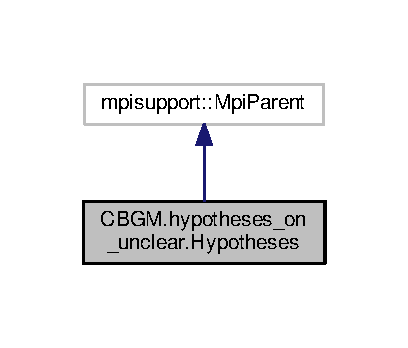
\includegraphics[width=196pt]{classCBGM_1_1hypotheses__on__unclear_1_1Hypotheses__inherit__graph}
\end{center}
\end{figure}


Collaboration diagram for C\+B\+G\+M.\+hypotheses\+\_\+on\+\_\+unclear.\+Hypotheses\+:\nopagebreak
\begin{figure}[H]
\begin{center}
\leavevmode
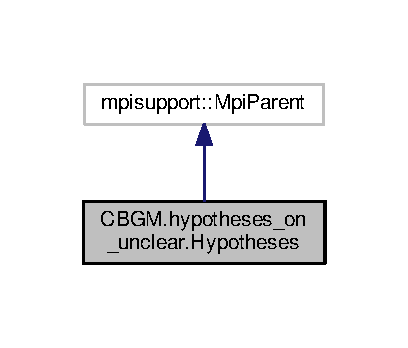
\includegraphics[width=196pt]{classCBGM_1_1hypotheses__on__unclear_1_1Hypotheses__coll__graph}
\end{center}
\end{figure}
\subsection*{Public Member Functions}
\begin{DoxyCompactItemize}
\item 
\mbox{\Hypertarget{classCBGM_1_1hypotheses__on__unclear_1_1Hypotheses_a938d4a5e8893f1f4400bce3b9d94b0a7}\label{classCBGM_1_1hypotheses__on__unclear_1_1Hypotheses_a938d4a5e8893f1f4400bce3b9d94b0a7}} 
def {\bfseries \+\_\+\+\_\+init\+\_\+\+\_\+} (self, data, all\+\_\+mss, vu, force=False, perfect\+\_\+only=True, connectivity=499, mpi=False)
\item 
def \hyperlink{classCBGM_1_1hypotheses__on__unclear_1_1Hypotheses_a1a3028848ce6ab8da0dde0036194d42d}{hypotheses} (self)
\item 
def \hyperlink{classCBGM_1_1hypotheses__on__unclear_1_1Hypotheses_ac4520130ea50d36145e8bcd963ddc40d}{mpi\+\_\+handle\+\_\+result} (self, args, ret)
\end{DoxyCompactItemize}
\subsection*{Public Attributes}
\begin{DoxyCompactItemize}
\item 
\mbox{\Hypertarget{classCBGM_1_1hypotheses__on__unclear_1_1Hypotheses_a6cec7a3f8b9aec69b325993ead0712ff}\label{classCBGM_1_1hypotheses__on__unclear_1_1Hypotheses_a6cec7a3f8b9aec69b325993ead0712ff}} 
{\bfseries data}
\item 
\mbox{\Hypertarget{classCBGM_1_1hypotheses__on__unclear_1_1Hypotheses_a8cd98f47c6ce3d3975485fd8fdee13ea}\label{classCBGM_1_1hypotheses__on__unclear_1_1Hypotheses_a8cd98f47c6ce3d3975485fd8fdee13ea}} 
{\bfseries all\+\_\+mss}
\item 
\mbox{\Hypertarget{classCBGM_1_1hypotheses__on__unclear_1_1Hypotheses_aaf64a1f837cbcd3c362bc1119df008d4}\label{classCBGM_1_1hypotheses__on__unclear_1_1Hypotheses_aaf64a1f837cbcd3c362bc1119df008d4}} 
{\bfseries vu}
\item 
\mbox{\Hypertarget{classCBGM_1_1hypotheses__on__unclear_1_1Hypotheses_a9b75dc7470edcbe149bc8c79b04f17b2}\label{classCBGM_1_1hypotheses__on__unclear_1_1Hypotheses_a9b75dc7470edcbe149bc8c79b04f17b2}} 
{\bfseries force}
\item 
\mbox{\Hypertarget{classCBGM_1_1hypotheses__on__unclear_1_1Hypotheses_add71f22f9d2c2129d9b731f0c1d94c81}\label{classCBGM_1_1hypotheses__on__unclear_1_1Hypotheses_add71f22f9d2c2129d9b731f0c1d94c81}} 
{\bfseries perfect\+\_\+only}
\item 
\mbox{\Hypertarget{classCBGM_1_1hypotheses__on__unclear_1_1Hypotheses_a3a61d8f28990d96eefe266b1b72be6e7}\label{classCBGM_1_1hypotheses__on__unclear_1_1Hypotheses_a3a61d8f28990d96eefe266b1b72be6e7}} 
{\bfseries connectivity}
\item 
\mbox{\Hypertarget{classCBGM_1_1hypotheses__on__unclear_1_1Hypotheses_adea67f80f7a34d8c426df748872306e0}\label{classCBGM_1_1hypotheses__on__unclear_1_1Hypotheses_adea67f80f7a34d8c426df748872306e0}} 
{\bfseries results}
\item 
\mbox{\Hypertarget{classCBGM_1_1hypotheses__on__unclear_1_1Hypotheses_ab5d3a83d6aaa116ac3e2292c02cb67f7}\label{classCBGM_1_1hypotheses__on__unclear_1_1Hypotheses_ab5d3a83d6aaa116ac3e2292c02cb67f7}} 
{\bfseries working\+\_\+dir}
\item 
\mbox{\Hypertarget{classCBGM_1_1hypotheses__on__unclear_1_1Hypotheses_a55bd2ba88fed965ce3027e3b94ad5d9a}\label{classCBGM_1_1hypotheses__on__unclear_1_1Hypotheses_a55bd2ba88fed965ce3027e3b94ad5d9a}} 
{\bfseries mpi}
\end{DoxyCompactItemize}


\subsection{Member Function Documentation}
\mbox{\Hypertarget{classCBGM_1_1hypotheses__on__unclear_1_1Hypotheses_a1a3028848ce6ab8da0dde0036194d42d}\label{classCBGM_1_1hypotheses__on__unclear_1_1Hypotheses_a1a3028848ce6ab8da0dde0036194d42d}} 
\index{C\+B\+G\+M\+::hypotheses\+\_\+on\+\_\+unclear\+::\+Hypotheses@{C\+B\+G\+M\+::hypotheses\+\_\+on\+\_\+unclear\+::\+Hypotheses}!hypotheses@{hypotheses}}
\index{hypotheses@{hypotheses}!C\+B\+G\+M\+::hypotheses\+\_\+on\+\_\+unclear\+::\+Hypotheses@{C\+B\+G\+M\+::hypotheses\+\_\+on\+\_\+unclear\+::\+Hypotheses}}
\subsubsection{\texorpdfstring{hypotheses()}{hypotheses()}}
{\footnotesize\ttfamily def C\+B\+G\+M.\+hypotheses\+\_\+on\+\_\+unclear.\+Hypotheses.\+hypotheses (\begin{DoxyParamCaption}\item[{}]{self }\end{DoxyParamCaption})}

\begin{DoxyVerb}Take a variant unit and create an html page with textual flow diagrams for all
potential hypotheses for UNCL readings.
\end{DoxyVerb}
 \mbox{\Hypertarget{classCBGM_1_1hypotheses__on__unclear_1_1Hypotheses_ac4520130ea50d36145e8bcd963ddc40d}\label{classCBGM_1_1hypotheses__on__unclear_1_1Hypotheses_ac4520130ea50d36145e8bcd963ddc40d}} 
\index{C\+B\+G\+M\+::hypotheses\+\_\+on\+\_\+unclear\+::\+Hypotheses@{C\+B\+G\+M\+::hypotheses\+\_\+on\+\_\+unclear\+::\+Hypotheses}!mpi\+\_\+handle\+\_\+result@{mpi\+\_\+handle\+\_\+result}}
\index{mpi\+\_\+handle\+\_\+result@{mpi\+\_\+handle\+\_\+result}!C\+B\+G\+M\+::hypotheses\+\_\+on\+\_\+unclear\+::\+Hypotheses@{C\+B\+G\+M\+::hypotheses\+\_\+on\+\_\+unclear\+::\+Hypotheses}}
\subsubsection{\texorpdfstring{mpi\+\_\+handle\+\_\+result()}{mpi\_handle\_result()}}
{\footnotesize\ttfamily def C\+B\+G\+M.\+hypotheses\+\_\+on\+\_\+unclear.\+Hypotheses.\+mpi\+\_\+handle\+\_\+result (\begin{DoxyParamCaption}\item[{}]{self,  }\item[{}]{args,  }\item[{}]{ret }\end{DoxyParamCaption})}

\begin{DoxyVerb}Handle an MPI result
@param args: original args sent to the child
@param ret: response from the child
\end{DoxyVerb}
 

The documentation for this class was generated from the following file\+:\begin{DoxyCompactItemize}
\item 
hypotheses\+\_\+on\+\_\+unclear.\+py\end{DoxyCompactItemize}

\hypertarget{classCBGM_1_1stripes_1_1LabelMapper}{}\section{C\+B\+G\+M.\+stripes.\+Label\+Mapper Class Reference}
\label{classCBGM_1_1stripes_1_1LabelMapper}\index{C\+B\+G\+M.\+stripes.\+Label\+Mapper@{C\+B\+G\+M.\+stripes.\+Label\+Mapper}}


Inheritance diagram for C\+B\+G\+M.\+stripes.\+Label\+Mapper\+:\nopagebreak
\begin{figure}[H]
\begin{center}
\leavevmode
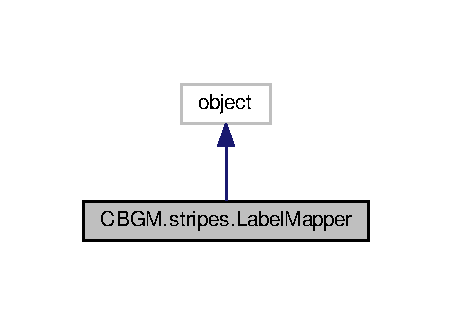
\includegraphics[width=217pt]{classCBGM_1_1stripes_1_1LabelMapper__inherit__graph}
\end{center}
\end{figure}


Collaboration diagram for C\+B\+G\+M.\+stripes.\+Label\+Mapper\+:\nopagebreak
\begin{figure}[H]
\begin{center}
\leavevmode
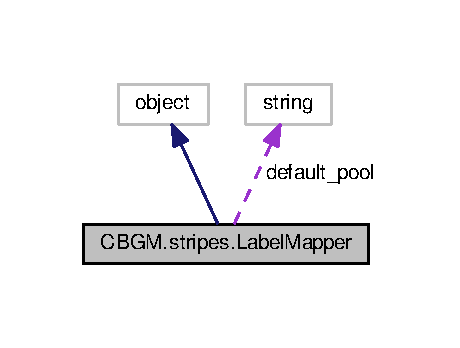
\includegraphics[width=221pt]{classCBGM_1_1stripes_1_1LabelMapper__coll__graph}
\end{center}
\end{figure}
\subsection*{Public Member Functions}
\begin{DoxyCompactItemize}
\item 
\mbox{\Hypertarget{classCBGM_1_1stripes_1_1LabelMapper_aa2992ee2fb7885dc67e30626433ab467}\label{classCBGM_1_1stripes_1_1LabelMapper_aa2992ee2fb7885dc67e30626433ab467}} 
def {\bfseries \+\_\+\+\_\+init\+\_\+\+\_\+} (self, pool=None)
\item 
\mbox{\Hypertarget{classCBGM_1_1stripes_1_1LabelMapper_a1e285e1fd2db5f10cacf4e18e7f688cf}\label{classCBGM_1_1stripes_1_1LabelMapper_a1e285e1fd2db5f10cacf4e18e7f688cf}} 
def {\bfseries get\+\_\+single\+\_\+char} (self, variant\+\_\+unit, label)
\end{DoxyCompactItemize}
\subsection*{Public Attributes}
\begin{DoxyCompactItemize}
\item 
\mbox{\Hypertarget{classCBGM_1_1stripes_1_1LabelMapper_a8bff3226952923179963889b8ff1de77}\label{classCBGM_1_1stripes_1_1LabelMapper_a8bff3226952923179963889b8ff1de77}} 
{\bfseries mapping}
\item 
\mbox{\Hypertarget{classCBGM_1_1stripes_1_1LabelMapper_a24964fac9f649f238a77359738861b90}\label{classCBGM_1_1stripes_1_1LabelMapper_a24964fac9f649f238a77359738861b90}} 
{\bfseries pool\+\_\+next}
\item 
\mbox{\Hypertarget{classCBGM_1_1stripes_1_1LabelMapper_a1a66c88dc0b3f3f41ca33ca7efc7d018}\label{classCBGM_1_1stripes_1_1LabelMapper_a1a66c88dc0b3f3f41ca33ca7efc7d018}} 
{\bfseries pool}
\end{DoxyCompactItemize}
\subsection*{Static Public Attributes}
\begin{DoxyCompactItemize}
\item 
\mbox{\Hypertarget{classCBGM_1_1stripes_1_1LabelMapper_a4cdba0dcd7009342c411877298f41d2d}\label{classCBGM_1_1stripes_1_1LabelMapper_a4cdba0dcd7009342c411877298f41d2d}} 
string {\bfseries default\+\_\+pool} = \textquotesingle{}αβγδεζηθκλμνξπρστυφχψω\textquotesingle{}
\end{DoxyCompactItemize}


The documentation for this class was generated from the following file\+:\begin{DoxyCompactItemize}
\item 
stripes.\+py\end{DoxyCompactItemize}

\hypertarget{classCBGM_1_1populate__db_1_1LacunaReading}{}\section{C\+B\+G\+M.\+populate\+\_\+db.\+Lacuna\+Reading Class Reference}
\label{classCBGM_1_1populate__db_1_1LacunaReading}\index{C\+B\+G\+M.\+populate\+\_\+db.\+Lacuna\+Reading@{C\+B\+G\+M.\+populate\+\_\+db.\+Lacuna\+Reading}}


Inheritance diagram for C\+B\+G\+M.\+populate\+\_\+db.\+Lacuna\+Reading\+:\nopagebreak
\begin{figure}[H]
\begin{center}
\leavevmode
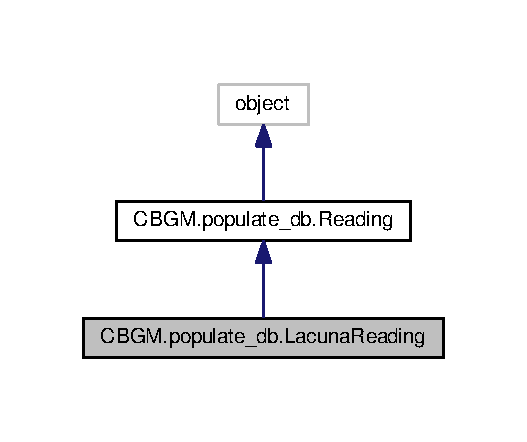
\includegraphics[width=253pt]{classCBGM_1_1populate__db_1_1LacunaReading__inherit__graph}
\end{center}
\end{figure}


Collaboration diagram for C\+B\+G\+M.\+populate\+\_\+db.\+Lacuna\+Reading\+:\nopagebreak
\begin{figure}[H]
\begin{center}
\leavevmode
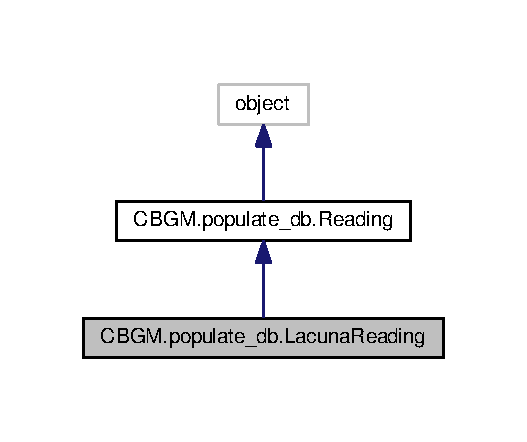
\includegraphics[width=253pt]{classCBGM_1_1populate__db_1_1LacunaReading__coll__graph}
\end{center}
\end{figure}
\subsection*{Public Member Functions}
\begin{DoxyCompactItemize}
\item 
\mbox{\Hypertarget{classCBGM_1_1populate__db_1_1LacunaReading_a33efe72a86dd1f989b51e358f41cd5b4}\label{classCBGM_1_1populate__db_1_1LacunaReading_a33efe72a86dd1f989b51e358f41cd5b4}} 
def {\bfseries \+\_\+\+\_\+init\+\_\+\+\_\+} (self, ms\+\_\+support)
\end{DoxyCompactItemize}
\subsection*{Public Attributes}
\begin{DoxyCompactItemize}
\item 
\mbox{\Hypertarget{classCBGM_1_1populate__db_1_1LacunaReading_a1abf40c9cbdbf175a146a70368ff2758}\label{classCBGM_1_1populate__db_1_1LacunaReading_a1abf40c9cbdbf175a146a70368ff2758}} 
{\bfseries ms\+\_\+support}
\item 
\mbox{\Hypertarget{classCBGM_1_1populate__db_1_1LacunaReading_a2c93f9c12970d94fcd70e2a669a9ed8c}\label{classCBGM_1_1populate__db_1_1LacunaReading_a2c93f9c12970d94fcd70e2a669a9ed8c}} 
{\bfseries lacuna}
\item 
\mbox{\Hypertarget{classCBGM_1_1populate__db_1_1LacunaReading_a9552c1d698d061f05ff92c0c380e9546}\label{classCBGM_1_1populate__db_1_1LacunaReading_a9552c1d698d061f05ff92c0c380e9546}} 
{\bfseries label}
\item 
\mbox{\Hypertarget{classCBGM_1_1populate__db_1_1LacunaReading_a4253a4c06320743e9951c48558a99b05}\label{classCBGM_1_1populate__db_1_1LacunaReading_a4253a4c06320743e9951c48558a99b05}} 
{\bfseries parent}
\end{DoxyCompactItemize}


The documentation for this class was generated from the following file\+:\begin{DoxyCompactItemize}
\item 
populate\+\_\+db.\+py\end{DoxyCompactItemize}

\hypertarget{classCBGM_1_1lib_1_1combinations__of__ancestors_1_1MpiHandler}{}\section{C\+B\+G\+M.\+lib.\+combinations\+\_\+of\+\_\+ancestors.\+Mpi\+Handler Class Reference}
\label{classCBGM_1_1lib_1_1combinations__of__ancestors_1_1MpiHandler}\index{C\+B\+G\+M.\+lib.\+combinations\+\_\+of\+\_\+ancestors.\+Mpi\+Handler@{C\+B\+G\+M.\+lib.\+combinations\+\_\+of\+\_\+ancestors.\+Mpi\+Handler}}


Inheritance diagram for C\+B\+G\+M.\+lib.\+combinations\+\_\+of\+\_\+ancestors.\+Mpi\+Handler\+:\nopagebreak
\begin{figure}[H]
\begin{center}
\leavevmode
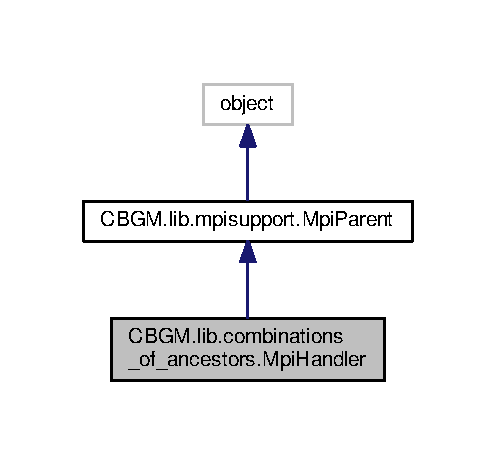
\includegraphics[width=238pt]{classCBGM_1_1lib_1_1combinations__of__ancestors_1_1MpiHandler__inherit__graph}
\end{center}
\end{figure}


Collaboration diagram for C\+B\+G\+M.\+lib.\+combinations\+\_\+of\+\_\+ancestors.\+Mpi\+Handler\+:\nopagebreak
\begin{figure}[H]
\begin{center}
\leavevmode
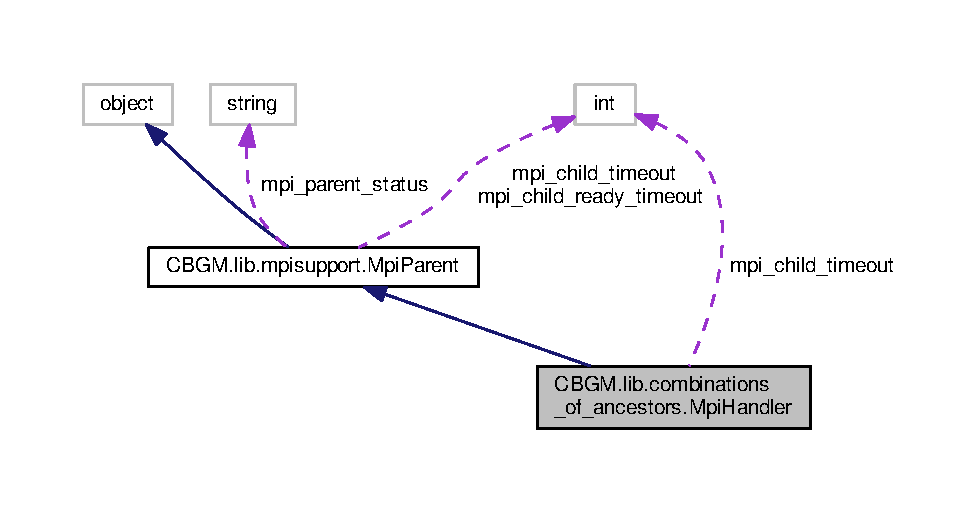
\includegraphics[width=350pt]{classCBGM_1_1lib_1_1combinations__of__ancestors_1_1MpiHandler__coll__graph}
\end{center}
\end{figure}
\subsection*{Public Member Functions}
\begin{DoxyCompactItemize}
\item 
def \hyperlink{classCBGM_1_1lib_1_1combinations__of__ancestors_1_1MpiHandler_a2a59dbe4025f51463eb1e8c148a3399c}{mpi\+\_\+handle\+\_\+result} (self, args, ret)
\end{DoxyCompactItemize}
\subsection*{Static Public Attributes}
\begin{DoxyCompactItemize}
\item 
\mbox{\Hypertarget{classCBGM_1_1lib_1_1combinations__of__ancestors_1_1MpiHandler_a78dba6ee5fcff75c4f59875ca76dd378}\label{classCBGM_1_1lib_1_1combinations__of__ancestors_1_1MpiHandler_a78dba6ee5fcff75c4f59875ca76dd378}} 
int {\bfseries mpi\+\_\+child\+\_\+timeout} = 3600 $\ast$ 4
\end{DoxyCompactItemize}
\subsection*{Additional Inherited Members}


\subsection{Member Function Documentation}
\mbox{\Hypertarget{classCBGM_1_1lib_1_1combinations__of__ancestors_1_1MpiHandler_a2a59dbe4025f51463eb1e8c148a3399c}\label{classCBGM_1_1lib_1_1combinations__of__ancestors_1_1MpiHandler_a2a59dbe4025f51463eb1e8c148a3399c}} 
\index{C\+B\+G\+M\+::lib\+::combinations\+\_\+of\+\_\+ancestors\+::\+Mpi\+Handler@{C\+B\+G\+M\+::lib\+::combinations\+\_\+of\+\_\+ancestors\+::\+Mpi\+Handler}!mpi\+\_\+handle\+\_\+result@{mpi\+\_\+handle\+\_\+result}}
\index{mpi\+\_\+handle\+\_\+result@{mpi\+\_\+handle\+\_\+result}!C\+B\+G\+M\+::lib\+::combinations\+\_\+of\+\_\+ancestors\+::\+Mpi\+Handler@{C\+B\+G\+M\+::lib\+::combinations\+\_\+of\+\_\+ancestors\+::\+Mpi\+Handler}}
\subsubsection{\texorpdfstring{mpi\+\_\+handle\+\_\+result()}{mpi\_handle\_result()}}
{\footnotesize\ttfamily def C\+B\+G\+M.\+lib.\+combinations\+\_\+of\+\_\+ancestors.\+Mpi\+Handler.\+mpi\+\_\+handle\+\_\+result (\begin{DoxyParamCaption}\item[{}]{self,  }\item[{}]{args,  }\item[{}]{ret }\end{DoxyParamCaption})}

\begin{DoxyVerb}Handle an MPI result
@param args: original args sent to the child
@param ret: response from the child
\end{DoxyVerb}
 

The documentation for this class was generated from the following file\+:\begin{DoxyCompactItemize}
\item 
lib/combinations\+\_\+of\+\_\+ancestors.\+py\end{DoxyCompactItemize}

\hypertarget{classCBGM_1_1lib_1_1textual__flow_1_1MpiHandler}{}\section{C\+B\+G\+M.\+lib.\+textual\+\_\+flow.\+Mpi\+Handler Class Reference}
\label{classCBGM_1_1lib_1_1textual__flow_1_1MpiHandler}\index{C\+B\+G\+M.\+lib.\+textual\+\_\+flow.\+Mpi\+Handler@{C\+B\+G\+M.\+lib.\+textual\+\_\+flow.\+Mpi\+Handler}}


Inheritance diagram for C\+B\+G\+M.\+lib.\+textual\+\_\+flow.\+Mpi\+Handler\+:\nopagebreak
\begin{figure}[H]
\begin{center}
\leavevmode
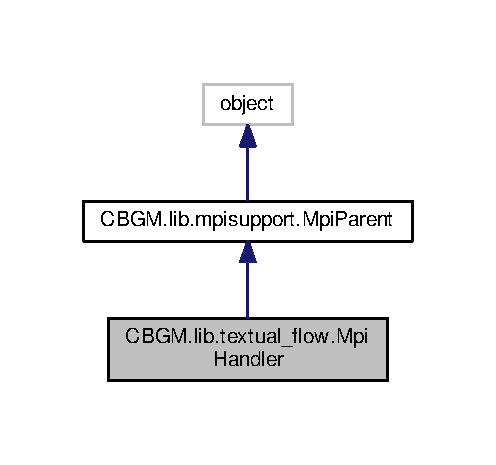
\includegraphics[width=238pt]{classCBGM_1_1lib_1_1textual__flow_1_1MpiHandler__inherit__graph}
\end{center}
\end{figure}


Collaboration diagram for C\+B\+G\+M.\+lib.\+textual\+\_\+flow.\+Mpi\+Handler\+:\nopagebreak
\begin{figure}[H]
\begin{center}
\leavevmode
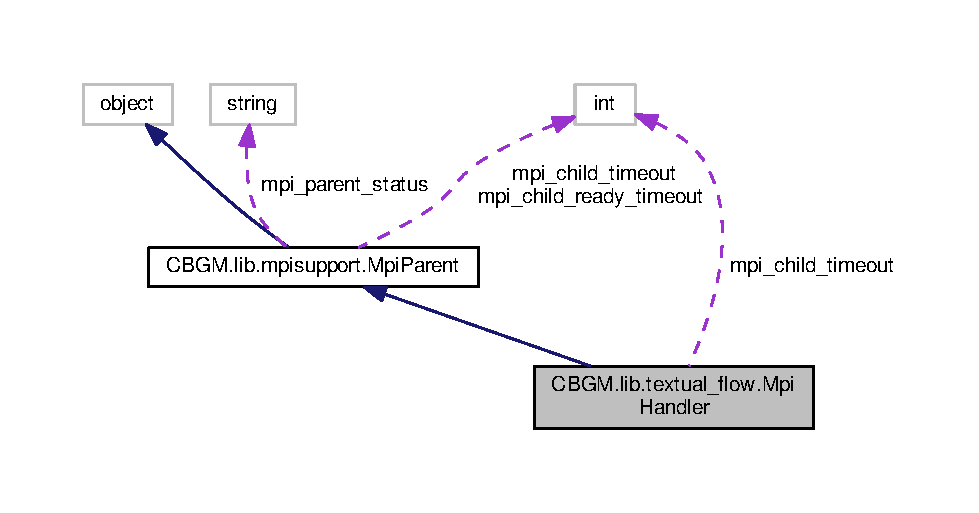
\includegraphics[width=350pt]{classCBGM_1_1lib_1_1textual__flow_1_1MpiHandler__coll__graph}
\end{center}
\end{figure}
\subsection*{Public Member Functions}
\begin{DoxyCompactItemize}
\item 
\mbox{\Hypertarget{classCBGM_1_1lib_1_1textual__flow_1_1MpiHandler_a3e1d8d0e16343d1b40a9adc9dd2eccc6}\label{classCBGM_1_1lib_1_1textual__flow_1_1MpiHandler_a3e1d8d0e16343d1b40a9adc9dd2eccc6}} 
def {\bfseries \+\_\+\+\_\+init\+\_\+\+\_\+} (self)
\item 
def \hyperlink{classCBGM_1_1lib_1_1textual__flow_1_1MpiHandler_a866c669ed6a88f73639cb286582582db}{queue\+\_\+textual\+\_\+flow} (self, vu, kwargs)
\item 
def \hyperlink{classCBGM_1_1lib_1_1textual__flow_1_1MpiHandler_a886c86704d9eda0327d5cf0c9be5b642}{done} (self, vu)
\item 
def \hyperlink{classCBGM_1_1lib_1_1textual__flow_1_1MpiHandler_acce71484acbf342eb74a73b1a663c188}{mpi\+\_\+handle\+\_\+result} (self, args, ret)
\end{DoxyCompactItemize}
\subsection*{Public Attributes}
\begin{DoxyCompactItemize}
\item 
\mbox{\Hypertarget{classCBGM_1_1lib_1_1textual__flow_1_1MpiHandler_a4088373003a58f5f72502a940149a609}\label{classCBGM_1_1lib_1_1textual__flow_1_1MpiHandler_a4088373003a58f5f72502a940149a609}} 
{\bfseries textual\+\_\+flow\+\_\+objects}
\end{DoxyCompactItemize}
\subsection*{Static Public Attributes}
\begin{DoxyCompactItemize}
\item 
\mbox{\Hypertarget{classCBGM_1_1lib_1_1textual__flow_1_1MpiHandler_abab146805ac64b7806ecc9814d08da97}\label{classCBGM_1_1lib_1_1textual__flow_1_1MpiHandler_abab146805ac64b7806ecc9814d08da97}} 
int {\bfseries mpi\+\_\+child\+\_\+timeout} = 3600 $\ast$ 4
\end{DoxyCompactItemize}


\subsection{Member Function Documentation}
\mbox{\Hypertarget{classCBGM_1_1lib_1_1textual__flow_1_1MpiHandler_a886c86704d9eda0327d5cf0c9be5b642}\label{classCBGM_1_1lib_1_1textual__flow_1_1MpiHandler_a886c86704d9eda0327d5cf0c9be5b642}} 
\index{C\+B\+G\+M\+::lib\+::textual\+\_\+flow\+::\+Mpi\+Handler@{C\+B\+G\+M\+::lib\+::textual\+\_\+flow\+::\+Mpi\+Handler}!done@{done}}
\index{done@{done}!C\+B\+G\+M\+::lib\+::textual\+\_\+flow\+::\+Mpi\+Handler@{C\+B\+G\+M\+::lib\+::textual\+\_\+flow\+::\+Mpi\+Handler}}
\subsubsection{\texorpdfstring{done()}{done()}}
{\footnotesize\ttfamily def C\+B\+G\+M.\+lib.\+textual\+\_\+flow.\+Mpi\+Handler.\+done (\begin{DoxyParamCaption}\item[{}]{self,  }\item[{}]{vu }\end{DoxyParamCaption})}

\begin{DoxyVerb}Finished with this VU - so lose the reference and let python free
up some memory.
\end{DoxyVerb}
 \mbox{\Hypertarget{classCBGM_1_1lib_1_1textual__flow_1_1MpiHandler_acce71484acbf342eb74a73b1a663c188}\label{classCBGM_1_1lib_1_1textual__flow_1_1MpiHandler_acce71484acbf342eb74a73b1a663c188}} 
\index{C\+B\+G\+M\+::lib\+::textual\+\_\+flow\+::\+Mpi\+Handler@{C\+B\+G\+M\+::lib\+::textual\+\_\+flow\+::\+Mpi\+Handler}!mpi\+\_\+handle\+\_\+result@{mpi\+\_\+handle\+\_\+result}}
\index{mpi\+\_\+handle\+\_\+result@{mpi\+\_\+handle\+\_\+result}!C\+B\+G\+M\+::lib\+::textual\+\_\+flow\+::\+Mpi\+Handler@{C\+B\+G\+M\+::lib\+::textual\+\_\+flow\+::\+Mpi\+Handler}}
\subsubsection{\texorpdfstring{mpi\+\_\+handle\+\_\+result()}{mpi\_handle\_result()}}
{\footnotesize\ttfamily def C\+B\+G\+M.\+lib.\+textual\+\_\+flow.\+Mpi\+Handler.\+mpi\+\_\+handle\+\_\+result (\begin{DoxyParamCaption}\item[{}]{self,  }\item[{}]{args,  }\item[{}]{ret }\end{DoxyParamCaption})}

\begin{DoxyVerb}Handle an MPI result
@param args: original args sent to the child
@param ret: response from the child
\end{DoxyVerb}
 \mbox{\Hypertarget{classCBGM_1_1lib_1_1textual__flow_1_1MpiHandler_a866c669ed6a88f73639cb286582582db}\label{classCBGM_1_1lib_1_1textual__flow_1_1MpiHandler_a866c669ed6a88f73639cb286582582db}} 
\index{C\+B\+G\+M\+::lib\+::textual\+\_\+flow\+::\+Mpi\+Handler@{C\+B\+G\+M\+::lib\+::textual\+\_\+flow\+::\+Mpi\+Handler}!queue\+\_\+textual\+\_\+flow@{queue\+\_\+textual\+\_\+flow}}
\index{queue\+\_\+textual\+\_\+flow@{queue\+\_\+textual\+\_\+flow}!C\+B\+G\+M\+::lib\+::textual\+\_\+flow\+::\+Mpi\+Handler@{C\+B\+G\+M\+::lib\+::textual\+\_\+flow\+::\+Mpi\+Handler}}
\subsubsection{\texorpdfstring{queue\+\_\+textual\+\_\+flow()}{queue\_textual\_flow()}}
{\footnotesize\ttfamily def C\+B\+G\+M.\+lib.\+textual\+\_\+flow.\+Mpi\+Handler.\+queue\+\_\+textual\+\_\+flow (\begin{DoxyParamCaption}\item[{}]{self,  }\item[{}]{vu,  }\item[{}]{kwargs }\end{DoxyParamCaption})}

\begin{DoxyVerb}Make a TextualFlow object, and get it to queue up all its MPI work.
\end{DoxyVerb}
 

The documentation for this class was generated from the following file\+:\begin{DoxyCompactItemize}
\item 
lib/textual\+\_\+flow.\+py\end{DoxyCompactItemize}

\hypertarget{classCBGM_1_1lib_1_1mpisupport_1_1MpiParent}{}\section{C\+B\+G\+M.\+lib.\+mpisupport.\+Mpi\+Parent Class Reference}
\label{classCBGM_1_1lib_1_1mpisupport_1_1MpiParent}\index{C\+B\+G\+M.\+lib.\+mpisupport.\+Mpi\+Parent@{C\+B\+G\+M.\+lib.\+mpisupport.\+Mpi\+Parent}}


Inheritance diagram for C\+B\+G\+M.\+lib.\+mpisupport.\+Mpi\+Parent\+:\nopagebreak
\begin{figure}[H]
\begin{center}
\leavevmode
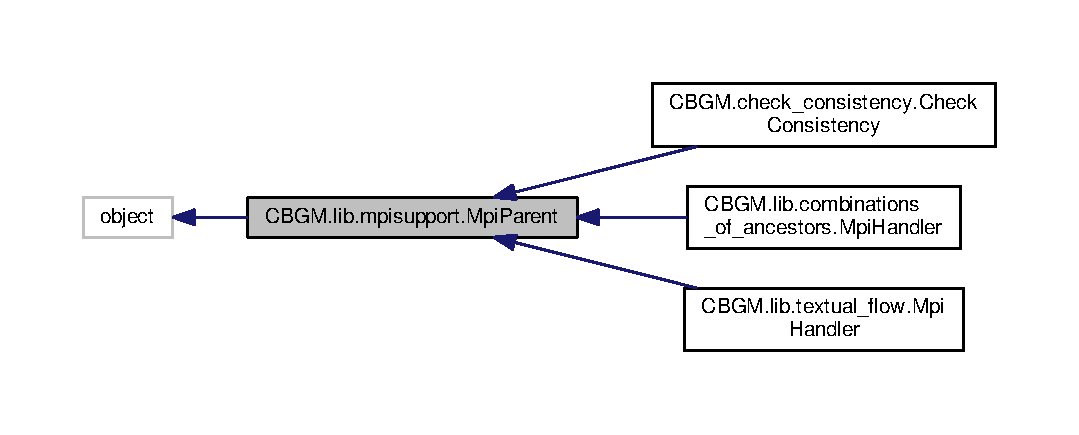
\includegraphics[width=350pt]{classCBGM_1_1lib_1_1mpisupport_1_1MpiParent__inherit__graph}
\end{center}
\end{figure}


Collaboration diagram for C\+B\+G\+M.\+lib.\+mpisupport.\+Mpi\+Parent\+:\nopagebreak
\begin{figure}[H]
\begin{center}
\leavevmode
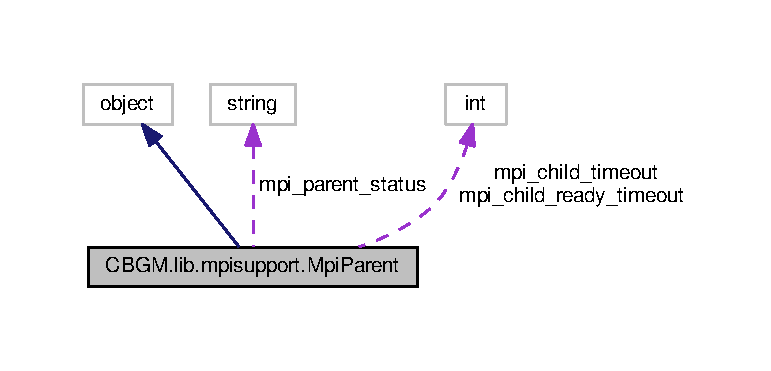
\includegraphics[width=350pt]{classCBGM_1_1lib_1_1mpisupport_1_1MpiParent__coll__graph}
\end{center}
\end{figure}
\subsection*{Public Member Functions}
\begin{DoxyCompactItemize}
\item 
\mbox{\Hypertarget{classCBGM_1_1lib_1_1mpisupport_1_1MpiParent_ae222e290d71602736a5898bdbfc67c27}\label{classCBGM_1_1lib_1_1mpisupport_1_1MpiParent_ae222e290d71602736a5898bdbfc67c27}} 
def {\bfseries \+\_\+\+\_\+init\+\_\+\+\_\+} (self)
\item 
def \hyperlink{classCBGM_1_1lib_1_1mpisupport_1_1MpiParent_ab70a1d7a4775e8b451f9c1797fc6c8c2}{mpi\+\_\+wait} (cls, stop=True)
\item 
\mbox{\Hypertarget{classCBGM_1_1lib_1_1mpisupport_1_1MpiParent_a4dc6c6972b31f1ef8f48d950926dcd68}\label{classCBGM_1_1lib_1_1mpisupport_1_1MpiParent_a4dc6c6972b31f1ef8f48d950926dcd68}} 
def {\bfseries show\+\_\+stats} (cls)
\item 
\mbox{\Hypertarget{classCBGM_1_1lib_1_1mpisupport_1_1MpiParent_a62195c4571b97756938cc673ee9df5c6}\label{classCBGM_1_1lib_1_1mpisupport_1_1MpiParent_a62195c4571b97756938cc673ee9df5c6}} 
def {\bfseries update\+\_\+parent\+\_\+stats} (cls, msg)
\item 
def \hyperlink{classCBGM_1_1lib_1_1mpisupport_1_1MpiParent_a70917e4e770c9997a04d74f9ac210f21}{mpi\+\_\+manage\+\_\+child} (cls, child)
\item 
def \hyperlink{classCBGM_1_1lib_1_1mpisupport_1_1MpiParent_ab421e046cec4458b87f5fb30a954dd40}{mpi\+\_\+handle\+\_\+result} (self, args, ret)
\item 
def \hyperlink{classCBGM_1_1lib_1_1mpisupport_1_1MpiParent_a223e2c29909cef0f2b08c8a608cdd117}{mpi\+\_\+run} (cls)
\item 
\mbox{\Hypertarget{classCBGM_1_1lib_1_1mpisupport_1_1MpiParent_a1b6a51bf09048a5b5d7eaf6fef542453}\label{classCBGM_1_1lib_1_1mpisupport_1_1MpiParent_a1b6a51bf09048a5b5d7eaf6fef542453}} 
def {\bfseries stats\+\_\+thread} (cls)
\end{DoxyCompactItemize}
\subsection*{Public Attributes}
\begin{DoxyCompactItemize}
\item 
\mbox{\Hypertarget{classCBGM_1_1lib_1_1mpisupport_1_1MpiParent_a0dc5bba031ec7057b82e3b96f62727a1}\label{classCBGM_1_1lib_1_1mpisupport_1_1MpiParent_a0dc5bba031ec7057b82e3b96f62727a1}} 
{\bfseries mpi\+\_\+child\+\_\+threads}
\item 
\mbox{\Hypertarget{classCBGM_1_1lib_1_1mpisupport_1_1MpiParent_ac764ad555f810dcafca1ed5726acfd3f}\label{classCBGM_1_1lib_1_1mpisupport_1_1MpiParent_ac764ad555f810dcafca1ed5726acfd3f}} 
{\bfseries mpi\+\_\+parent\+\_\+status}
\end{DoxyCompactItemize}
\subsection*{Static Public Attributes}
\begin{DoxyCompactItemize}
\item 
\mbox{\Hypertarget{classCBGM_1_1lib_1_1mpisupport_1_1MpiParent_a99faccf2560be14aa0a2ef61b216d1dc}\label{classCBGM_1_1lib_1_1mpisupport_1_1MpiParent_a99faccf2560be14aa0a2ef61b216d1dc}} 
{\bfseries mpicomm} = None
\item 
\mbox{\Hypertarget{classCBGM_1_1lib_1_1mpisupport_1_1MpiParent_a7660ab4833e80b610a152803b76d24cf}\label{classCBGM_1_1lib_1_1mpisupport_1_1MpiParent_a7660ab4833e80b610a152803b76d24cf}} 
{\bfseries mpi\+\_\+queue} = queue.\+Queue()
\item 
\mbox{\Hypertarget{classCBGM_1_1lib_1_1mpisupport_1_1MpiParent_ab0375a0afdd4360b53bcd4dc51e7d7ec}\label{classCBGM_1_1lib_1_1mpisupport_1_1MpiParent_ab0375a0afdd4360b53bcd4dc51e7d7ec}} 
list {\bfseries mpi\+\_\+child\+\_\+threads} = \mbox{[}$\,$\mbox{]}
\item 
\mbox{\Hypertarget{classCBGM_1_1lib_1_1mpisupport_1_1MpiParent_a216e95a0116a746cc8c53f73c909f335}\label{classCBGM_1_1lib_1_1mpisupport_1_1MpiParent_a216e95a0116a746cc8c53f73c909f335}} 
dictionary {\bfseries mpi\+\_\+child\+\_\+status} = \{\}
\item 
\mbox{\Hypertarget{classCBGM_1_1lib_1_1mpisupport_1_1MpiParent_accd35b8ffd377a2622e4a6053172eed6}\label{classCBGM_1_1lib_1_1mpisupport_1_1MpiParent_accd35b8ffd377a2622e4a6053172eed6}} 
dictionary {\bfseries mpi\+\_\+child\+\_\+meminfo} = \{\}
\item 
\mbox{\Hypertarget{classCBGM_1_1lib_1_1mpisupport_1_1MpiParent_aeff4e4f9ca63acf372cfd9ffa15533c3}\label{classCBGM_1_1lib_1_1mpisupport_1_1MpiParent_aeff4e4f9ca63acf372cfd9ffa15533c3}} 
int {\bfseries mpi\+\_\+child\+\_\+timeout} = 3600
\item 
\mbox{\Hypertarget{classCBGM_1_1lib_1_1mpisupport_1_1MpiParent_ad11dc15e8b1c8d5589808794f8ae96dd}\label{classCBGM_1_1lib_1_1mpisupport_1_1MpiParent_ad11dc15e8b1c8d5589808794f8ae96dd}} 
int {\bfseries mpi\+\_\+child\+\_\+ready\+\_\+timeout} = 30
\item 
\mbox{\Hypertarget{classCBGM_1_1lib_1_1mpisupport_1_1MpiParent_aa5a02f6ea4d6e740e455f683855b8a6c}\label{classCBGM_1_1lib_1_1mpisupport_1_1MpiParent_aa5a02f6ea4d6e740e455f683855b8a6c}} 
string {\bfseries mpi\+\_\+parent\+\_\+status} = \char`\"{}\char`\"{}
\item 
\mbox{\Hypertarget{classCBGM_1_1lib_1_1mpisupport_1_1MpiParent_afb8718f3dc3af5b8b7cbff9d6a829fee}\label{classCBGM_1_1lib_1_1mpisupport_1_1MpiParent_afb8718f3dc3af5b8b7cbff9d6a829fee}} 
{\bfseries latest\+\_\+instance} = None
\end{DoxyCompactItemize}


\subsection{Member Function Documentation}
\mbox{\Hypertarget{classCBGM_1_1lib_1_1mpisupport_1_1MpiParent_ab421e046cec4458b87f5fb30a954dd40}\label{classCBGM_1_1lib_1_1mpisupport_1_1MpiParent_ab421e046cec4458b87f5fb30a954dd40}} 
\index{C\+B\+G\+M\+::lib\+::mpisupport\+::\+Mpi\+Parent@{C\+B\+G\+M\+::lib\+::mpisupport\+::\+Mpi\+Parent}!mpi\+\_\+handle\+\_\+result@{mpi\+\_\+handle\+\_\+result}}
\index{mpi\+\_\+handle\+\_\+result@{mpi\+\_\+handle\+\_\+result}!C\+B\+G\+M\+::lib\+::mpisupport\+::\+Mpi\+Parent@{C\+B\+G\+M\+::lib\+::mpisupport\+::\+Mpi\+Parent}}
\subsubsection{\texorpdfstring{mpi\+\_\+handle\+\_\+result()}{mpi\_handle\_result()}}
{\footnotesize\ttfamily def C\+B\+G\+M.\+lib.\+mpisupport.\+Mpi\+Parent.\+mpi\+\_\+handle\+\_\+result (\begin{DoxyParamCaption}\item[{}]{self,  }\item[{}]{args,  }\item[{}]{ret }\end{DoxyParamCaption})}

\begin{DoxyVerb}Handle an MPI result
@param args: original args sent to the child
@param ret: response from the child
\end{DoxyVerb}
 \mbox{\Hypertarget{classCBGM_1_1lib_1_1mpisupport_1_1MpiParent_a70917e4e770c9997a04d74f9ac210f21}\label{classCBGM_1_1lib_1_1mpisupport_1_1MpiParent_a70917e4e770c9997a04d74f9ac210f21}} 
\index{C\+B\+G\+M\+::lib\+::mpisupport\+::\+Mpi\+Parent@{C\+B\+G\+M\+::lib\+::mpisupport\+::\+Mpi\+Parent}!mpi\+\_\+manage\+\_\+child@{mpi\+\_\+manage\+\_\+child}}
\index{mpi\+\_\+manage\+\_\+child@{mpi\+\_\+manage\+\_\+child}!C\+B\+G\+M\+::lib\+::mpisupport\+::\+Mpi\+Parent@{C\+B\+G\+M\+::lib\+::mpisupport\+::\+Mpi\+Parent}}
\subsubsection{\texorpdfstring{mpi\+\_\+manage\+\_\+child()}{mpi\_manage\_child()}}
{\footnotesize\ttfamily def C\+B\+G\+M.\+lib.\+mpisupport.\+Mpi\+Parent.\+mpi\+\_\+manage\+\_\+child (\begin{DoxyParamCaption}\item[{}]{cls,  }\item[{}]{child }\end{DoxyParamCaption})}

\begin{DoxyVerb}Manage communications with the specified MPI child
\end{DoxyVerb}
 \mbox{\Hypertarget{classCBGM_1_1lib_1_1mpisupport_1_1MpiParent_a223e2c29909cef0f2b08c8a608cdd117}\label{classCBGM_1_1lib_1_1mpisupport_1_1MpiParent_a223e2c29909cef0f2b08c8a608cdd117}} 
\index{C\+B\+G\+M\+::lib\+::mpisupport\+::\+Mpi\+Parent@{C\+B\+G\+M\+::lib\+::mpisupport\+::\+Mpi\+Parent}!mpi\+\_\+run@{mpi\+\_\+run}}
\index{mpi\+\_\+run@{mpi\+\_\+run}!C\+B\+G\+M\+::lib\+::mpisupport\+::\+Mpi\+Parent@{C\+B\+G\+M\+::lib\+::mpisupport\+::\+Mpi\+Parent}}
\subsubsection{\texorpdfstring{mpi\+\_\+run()}{mpi\_run()}}
{\footnotesize\ttfamily def C\+B\+G\+M.\+lib.\+mpisupport.\+Mpi\+Parent.\+mpi\+\_\+run (\begin{DoxyParamCaption}\item[{}]{cls }\end{DoxyParamCaption})}

\begin{DoxyVerb}Top-level MPI parent method.
\end{DoxyVerb}
 \mbox{\Hypertarget{classCBGM_1_1lib_1_1mpisupport_1_1MpiParent_ab70a1d7a4775e8b451f9c1797fc6c8c2}\label{classCBGM_1_1lib_1_1mpisupport_1_1MpiParent_ab70a1d7a4775e8b451f9c1797fc6c8c2}} 
\index{C\+B\+G\+M\+::lib\+::mpisupport\+::\+Mpi\+Parent@{C\+B\+G\+M\+::lib\+::mpisupport\+::\+Mpi\+Parent}!mpi\+\_\+wait@{mpi\+\_\+wait}}
\index{mpi\+\_\+wait@{mpi\+\_\+wait}!C\+B\+G\+M\+::lib\+::mpisupport\+::\+Mpi\+Parent@{C\+B\+G\+M\+::lib\+::mpisupport\+::\+Mpi\+Parent}}
\subsubsection{\texorpdfstring{mpi\+\_\+wait()}{mpi\_wait()}}
{\footnotesize\ttfamily def C\+B\+G\+M.\+lib.\+mpisupport.\+Mpi\+Parent.\+mpi\+\_\+wait (\begin{DoxyParamCaption}\item[{}]{cls,  }\item[{}]{stop = {\ttfamily True} }\end{DoxyParamCaption})}

\begin{DoxyVerb}Wait for all work to be done, then tell things to stop.

Make sure you've put things in the queue before calling this... or
it will all just exit and move on.
\end{DoxyVerb}
 

The documentation for this class was generated from the following file\+:\begin{DoxyCompactItemize}
\item 
lib/mpisupport.\+py\end{DoxyCompactItemize}

\hypertarget{classCBGM_1_1lib_1_1genealogical__coherence_1_1ParentCombination}{}\section{C\+B\+G\+M.\+lib.\+genealogical\+\_\+coherence.\+Parent\+Combination Class Reference}
\label{classCBGM_1_1lib_1_1genealogical__coherence_1_1ParentCombination}\index{C\+B\+G\+M.\+lib.\+genealogical\+\_\+coherence.\+Parent\+Combination@{C\+B\+G\+M.\+lib.\+genealogical\+\_\+coherence.\+Parent\+Combination}}


Inheritance diagram for C\+B\+G\+M.\+lib.\+genealogical\+\_\+coherence.\+Parent\+Combination\+:\nopagebreak
\begin{figure}[H]
\begin{center}
\leavevmode
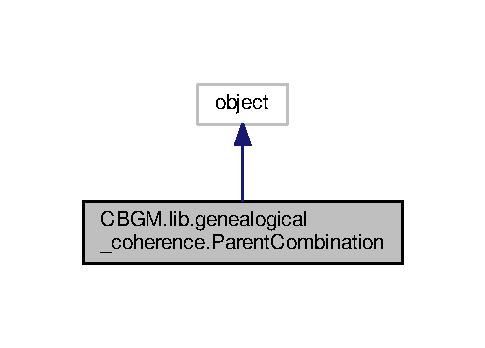
\includegraphics[width=233pt]{classCBGM_1_1lib_1_1genealogical__coherence_1_1ParentCombination__inherit__graph}
\end{center}
\end{figure}


Collaboration diagram for C\+B\+G\+M.\+lib.\+genealogical\+\_\+coherence.\+Parent\+Combination\+:\nopagebreak
\begin{figure}[H]
\begin{center}
\leavevmode
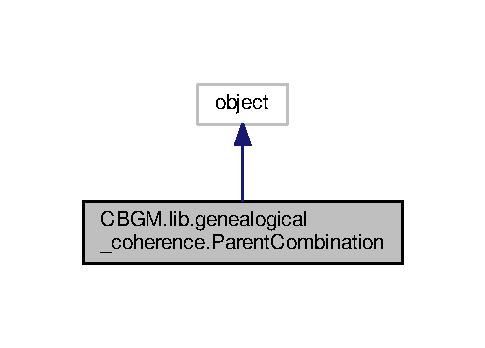
\includegraphics[width=233pt]{classCBGM_1_1lib_1_1genealogical__coherence_1_1ParentCombination__coll__graph}
\end{center}
\end{figure}
\subsection*{Public Member Functions}
\begin{DoxyCompactItemize}
\item 
\mbox{\Hypertarget{classCBGM_1_1lib_1_1genealogical__coherence_1_1ParentCombination_ad4a2f91478f4584db0b9c6c02a4be1f6}\label{classCBGM_1_1lib_1_1genealogical__coherence_1_1ParentCombination_ad4a2f91478f4584db0b9c6c02a4be1f6}} 
def {\bfseries \+\_\+\+\_\+init\+\_\+\+\_\+} (self, parent, rank, perc, gen, prior=None, posterior=None, undirected=False)
\item 
\mbox{\Hypertarget{classCBGM_1_1lib_1_1genealogical__coherence_1_1ParentCombination_a780833508a1774084d15d3840df5a839}\label{classCBGM_1_1lib_1_1genealogical__coherence_1_1ParentCombination_a780833508a1774084d15d3840df5a839}} 
def {\bfseries strength} (self)
\item 
\mbox{\Hypertarget{classCBGM_1_1lib_1_1genealogical__coherence_1_1ParentCombination_af655aba38d67c73cd2d1b7daeb6d287b}\label{classCBGM_1_1lib_1_1genealogical__coherence_1_1ParentCombination_af655aba38d67c73cd2d1b7daeb6d287b}} 
def {\bfseries \+\_\+\+\_\+repr\+\_\+\+\_\+} (self)
\end{DoxyCompactItemize}
\subsection*{Public Attributes}
\begin{DoxyCompactItemize}
\item 
\mbox{\Hypertarget{classCBGM_1_1lib_1_1genealogical__coherence_1_1ParentCombination_a06fcac22dc79f71577a4114c768e0650}\label{classCBGM_1_1lib_1_1genealogical__coherence_1_1ParentCombination_a06fcac22dc79f71577a4114c768e0650}} 
{\bfseries parent}
\item 
\mbox{\Hypertarget{classCBGM_1_1lib_1_1genealogical__coherence_1_1ParentCombination_a7463c4c0541a1e274814997c408aa2f8}\label{classCBGM_1_1lib_1_1genealogical__coherence_1_1ParentCombination_a7463c4c0541a1e274814997c408aa2f8}} 
{\bfseries rank}
\item 
\mbox{\Hypertarget{classCBGM_1_1lib_1_1genealogical__coherence_1_1ParentCombination_a1025008260cd678e36be274ada4a40e5}\label{classCBGM_1_1lib_1_1genealogical__coherence_1_1ParentCombination_a1025008260cd678e36be274ada4a40e5}} 
{\bfseries perc}
\item 
\mbox{\Hypertarget{classCBGM_1_1lib_1_1genealogical__coherence_1_1ParentCombination_a98a1a9a20aa05d5ad8489eb84513b5ea}\label{classCBGM_1_1lib_1_1genealogical__coherence_1_1ParentCombination_a98a1a9a20aa05d5ad8489eb84513b5ea}} 
{\bfseries gen}
\item 
\mbox{\Hypertarget{classCBGM_1_1lib_1_1genealogical__coherence_1_1ParentCombination_a0a79c415819f6097eaf906422bac3f13}\label{classCBGM_1_1lib_1_1genealogical__coherence_1_1ParentCombination_a0a79c415819f6097eaf906422bac3f13}} 
{\bfseries prior}
\item 
\mbox{\Hypertarget{classCBGM_1_1lib_1_1genealogical__coherence_1_1ParentCombination_a7a6bdf5ad97a8bad4ff3a2d78e689cf0}\label{classCBGM_1_1lib_1_1genealogical__coherence_1_1ParentCombination_a7a6bdf5ad97a8bad4ff3a2d78e689cf0}} 
{\bfseries posterior}
\item 
\mbox{\Hypertarget{classCBGM_1_1lib_1_1genealogical__coherence_1_1ParentCombination_a9b8e8ba79e16c5c26e5801ee296ada3a}\label{classCBGM_1_1lib_1_1genealogical__coherence_1_1ParentCombination_a9b8e8ba79e16c5c26e5801ee296ada3a}} 
{\bfseries undirected}
\end{DoxyCompactItemize}


The documentation for this class was generated from the following file\+:\begin{DoxyCompactItemize}
\item 
lib/genealogical\+\_\+coherence.\+py\end{DoxyCompactItemize}

\hypertarget{classCBGM_1_1populate__db_1_1Reading}{}\section{C\+B\+G\+M.\+populate\+\_\+db.\+Reading Class Reference}
\label{classCBGM_1_1populate__db_1_1Reading}\index{C\+B\+G\+M.\+populate\+\_\+db.\+Reading@{C\+B\+G\+M.\+populate\+\_\+db.\+Reading}}


Inheritance diagram for C\+B\+G\+M.\+populate\+\_\+db.\+Reading\+:\nopagebreak
\begin{figure}[H]
\begin{center}
\leavevmode
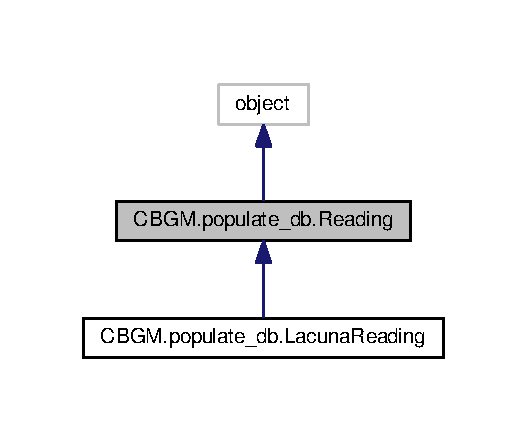
\includegraphics[width=253pt]{classCBGM_1_1populate__db_1_1Reading__inherit__graph}
\end{center}
\end{figure}


Collaboration diagram for C\+B\+G\+M.\+populate\+\_\+db.\+Reading\+:\nopagebreak
\begin{figure}[H]
\begin{center}
\leavevmode
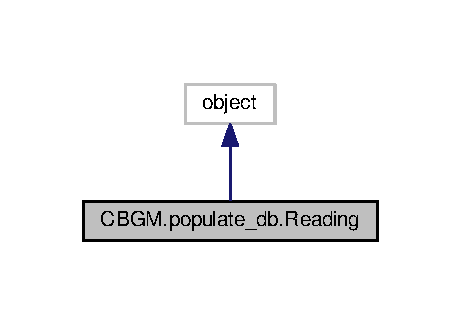
\includegraphics[width=221pt]{classCBGM_1_1populate__db_1_1Reading__coll__graph}
\end{center}
\end{figure}
\subsection*{Public Member Functions}
\begin{DoxyCompactItemize}
\item 
\mbox{\Hypertarget{classCBGM_1_1populate__db_1_1Reading_af4b405e7576f61acb0553afcd2b6a85d}\label{classCBGM_1_1populate__db_1_1Reading_af4b405e7576f61acb0553afcd2b6a85d}} 
def {\bfseries \+\_\+\+\_\+init\+\_\+\+\_\+} (self, label, greek, ms\+\_\+support, parent)
\item 
def \hyperlink{classCBGM_1_1populate__db_1_1Reading_a3bf5a41e1c3e75a3e68ccd875abaec14}{calc\+\_\+mss\+\_\+support} (self, all\+\_\+mss)
\item 
\mbox{\Hypertarget{classCBGM_1_1populate__db_1_1Reading_aa0541611a5e63b28be511424c00bf09a}\label{classCBGM_1_1populate__db_1_1Reading_aa0541611a5e63b28be511424c00bf09a}} 
def {\bfseries \+\_\+\+\_\+repr\+\_\+\+\_\+} (self)
\end{DoxyCompactItemize}
\subsection*{Public Attributes}
\begin{DoxyCompactItemize}
\item 
\mbox{\Hypertarget{classCBGM_1_1populate__db_1_1Reading_ad238a8f5526e3cefdd784db1832d33d6}\label{classCBGM_1_1populate__db_1_1Reading_ad238a8f5526e3cefdd784db1832d33d6}} 
{\bfseries lacuna}
\item 
\mbox{\Hypertarget{classCBGM_1_1populate__db_1_1Reading_ae8ed3c81e4b05935e656205b03be2cfe}\label{classCBGM_1_1populate__db_1_1Reading_ae8ed3c81e4b05935e656205b03be2cfe}} 
{\bfseries label}
\item 
\mbox{\Hypertarget{classCBGM_1_1populate__db_1_1Reading_a90156e434a18bf29c2566d2280eb4ddc}\label{classCBGM_1_1populate__db_1_1Reading_a90156e434a18bf29c2566d2280eb4ddc}} 
{\bfseries greek}
\item 
\mbox{\Hypertarget{classCBGM_1_1populate__db_1_1Reading_aa158d27362f00f933ea97fbcdc740a8e}\label{classCBGM_1_1populate__db_1_1Reading_aa158d27362f00f933ea97fbcdc740a8e}} 
{\bfseries ms\+\_\+support}
\item 
\mbox{\Hypertarget{classCBGM_1_1populate__db_1_1Reading_a27731d61c8271ae959a5c1b978b6fc22}\label{classCBGM_1_1populate__db_1_1Reading_a27731d61c8271ae959a5c1b978b6fc22}} 
{\bfseries parent}
\end{DoxyCompactItemize}


\subsection{Member Function Documentation}
\mbox{\Hypertarget{classCBGM_1_1populate__db_1_1Reading_a3bf5a41e1c3e75a3e68ccd875abaec14}\label{classCBGM_1_1populate__db_1_1Reading_a3bf5a41e1c3e75a3e68ccd875abaec14}} 
\index{C\+B\+G\+M\+::populate\+\_\+db\+::\+Reading@{C\+B\+G\+M\+::populate\+\_\+db\+::\+Reading}!calc\+\_\+mss\+\_\+support@{calc\+\_\+mss\+\_\+support}}
\index{calc\+\_\+mss\+\_\+support@{calc\+\_\+mss\+\_\+support}!C\+B\+G\+M\+::populate\+\_\+db\+::\+Reading@{C\+B\+G\+M\+::populate\+\_\+db\+::\+Reading}}
\subsubsection{\texorpdfstring{calc\+\_\+mss\+\_\+support()}{calc\_mss\_support()}}
{\footnotesize\ttfamily def C\+B\+G\+M.\+populate\+\_\+db.\+Reading.\+calc\+\_\+mss\+\_\+support (\begin{DoxyParamCaption}\item[{}]{self,  }\item[{}]{all\+\_\+mss }\end{DoxyParamCaption})}

\begin{DoxyVerb}Calculate manuscript support based on the list of all mss passed in
\end{DoxyVerb}
 

The documentation for this class was generated from the following file\+:\begin{DoxyCompactItemize}
\item 
populate\+\_\+db.\+py\end{DoxyCompactItemize}

\hypertarget{classCBGM_1_1lib_1_1genealogical__coherence_1_1ReadingRelationship}{}\section{C\+B\+G\+M.\+lib.\+genealogical\+\_\+coherence.\+Reading\+Relationship Class Reference}
\label{classCBGM_1_1lib_1_1genealogical__coherence_1_1ReadingRelationship}\index{C\+B\+G\+M.\+lib.\+genealogical\+\_\+coherence.\+Reading\+Relationship@{C\+B\+G\+M.\+lib.\+genealogical\+\_\+coherence.\+Reading\+Relationship}}


Inheritance diagram for C\+B\+G\+M.\+lib.\+genealogical\+\_\+coherence.\+Reading\+Relationship\+:\nopagebreak
\begin{figure}[H]
\begin{center}
\leavevmode
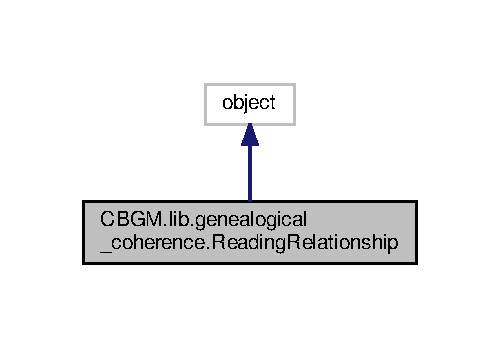
\includegraphics[width=240pt]{classCBGM_1_1lib_1_1genealogical__coherence_1_1ReadingRelationship__inherit__graph}
\end{center}
\end{figure}


Collaboration diagram for C\+B\+G\+M.\+lib.\+genealogical\+\_\+coherence.\+Reading\+Relationship\+:\nopagebreak
\begin{figure}[H]
\begin{center}
\leavevmode
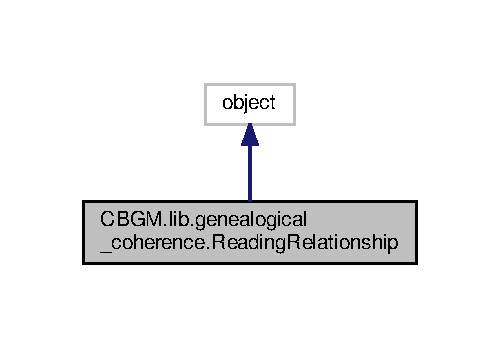
\includegraphics[width=240pt]{classCBGM_1_1lib_1_1genealogical__coherence_1_1ReadingRelationship__coll__graph}
\end{center}
\end{figure}
\subsection*{Public Member Functions}
\begin{DoxyCompactItemize}
\item 
\mbox{\Hypertarget{classCBGM_1_1lib_1_1genealogical__coherence_1_1ReadingRelationship_a081b8ca09a51fc4bea08f2d4cc956e6f}\label{classCBGM_1_1lib_1_1genealogical__coherence_1_1ReadingRelationship_a081b8ca09a51fc4bea08f2d4cc956e6f}} 
def {\bfseries \+\_\+\+\_\+init\+\_\+\+\_\+} (self, variant\+\_\+unit, reading, cursor)
\item 
def \hyperlink{classCBGM_1_1lib_1_1genealogical__coherence_1_1ReadingRelationship_a5c32a031e1f4f8aceffb2197786e0900}{identify\+\_\+relationship} (self, other\+\_\+reading)
\item 
def \hyperlink{classCBGM_1_1lib_1_1genealogical__coherence_1_1ReadingRelationship_a843113796c526603255efd6baf6b4d4d}{get\+\_\+parent\+\_\+reading} (self, reading)
\end{DoxyCompactItemize}
\subsection*{Public Attributes}
\begin{DoxyCompactItemize}
\item 
\mbox{\Hypertarget{classCBGM_1_1lib_1_1genealogical__coherence_1_1ReadingRelationship_a28c5f2c09bda27024688da9bb34829a7}\label{classCBGM_1_1lib_1_1genealogical__coherence_1_1ReadingRelationship_a28c5f2c09bda27024688da9bb34829a7}} 
{\bfseries variant\+\_\+unit}
\item 
\mbox{\Hypertarget{classCBGM_1_1lib_1_1genealogical__coherence_1_1ReadingRelationship_a17050690b94b94aa03ad91986c8b1663}\label{classCBGM_1_1lib_1_1genealogical__coherence_1_1ReadingRelationship_a17050690b94b94aa03ad91986c8b1663}} 
{\bfseries reading}
\item 
\mbox{\Hypertarget{classCBGM_1_1lib_1_1genealogical__coherence_1_1ReadingRelationship_a004519c3d54055e842265174d77d6e63}\label{classCBGM_1_1lib_1_1genealogical__coherence_1_1ReadingRelationship_a004519c3d54055e842265174d77d6e63}} 
{\bfseries cursor}
\end{DoxyCompactItemize}


\subsection{Detailed Description}
\begin{DoxyVerb}Class representing a reading in a specified variant unit.
\end{DoxyVerb}
 

\subsection{Member Function Documentation}
\mbox{\Hypertarget{classCBGM_1_1lib_1_1genealogical__coherence_1_1ReadingRelationship_a843113796c526603255efd6baf6b4d4d}\label{classCBGM_1_1lib_1_1genealogical__coherence_1_1ReadingRelationship_a843113796c526603255efd6baf6b4d4d}} 
\index{C\+B\+G\+M\+::lib\+::genealogical\+\_\+coherence\+::\+Reading\+Relationship@{C\+B\+G\+M\+::lib\+::genealogical\+\_\+coherence\+::\+Reading\+Relationship}!get\+\_\+parent\+\_\+reading@{get\+\_\+parent\+\_\+reading}}
\index{get\+\_\+parent\+\_\+reading@{get\+\_\+parent\+\_\+reading}!C\+B\+G\+M\+::lib\+::genealogical\+\_\+coherence\+::\+Reading\+Relationship@{C\+B\+G\+M\+::lib\+::genealogical\+\_\+coherence\+::\+Reading\+Relationship}}
\subsubsection{\texorpdfstring{get\+\_\+parent\+\_\+reading()}{get\_parent\_reading()}}
{\footnotesize\ttfamily def C\+B\+G\+M.\+lib.\+genealogical\+\_\+coherence.\+Reading\+Relationship.\+get\+\_\+parent\+\_\+reading (\begin{DoxyParamCaption}\item[{}]{self,  }\item[{}]{reading }\end{DoxyParamCaption})}

\begin{DoxyVerb}Get the parent reading for this reading
\end{DoxyVerb}
 \mbox{\Hypertarget{classCBGM_1_1lib_1_1genealogical__coherence_1_1ReadingRelationship_a5c32a031e1f4f8aceffb2197786e0900}\label{classCBGM_1_1lib_1_1genealogical__coherence_1_1ReadingRelationship_a5c32a031e1f4f8aceffb2197786e0900}} 
\index{C\+B\+G\+M\+::lib\+::genealogical\+\_\+coherence\+::\+Reading\+Relationship@{C\+B\+G\+M\+::lib\+::genealogical\+\_\+coherence\+::\+Reading\+Relationship}!identify\+\_\+relationship@{identify\+\_\+relationship}}
\index{identify\+\_\+relationship@{identify\+\_\+relationship}!C\+B\+G\+M\+::lib\+::genealogical\+\_\+coherence\+::\+Reading\+Relationship@{C\+B\+G\+M\+::lib\+::genealogical\+\_\+coherence\+::\+Reading\+Relationship}}
\subsubsection{\texorpdfstring{identify\+\_\+relationship()}{identify\_relationship()}}
{\footnotesize\ttfamily def C\+B\+G\+M.\+lib.\+genealogical\+\_\+coherence.\+Reading\+Relationship.\+identify\+\_\+relationship (\begin{DoxyParamCaption}\item[{}]{self,  }\item[{}]{other\+\_\+reading }\end{DoxyParamCaption})}

\begin{DoxyVerb}Find out how our reading is related to this other one

Returns EQUAL, PRIOR, POSTERIOR, UNCL or NOREL
\end{DoxyVerb}
 

The documentation for this class was generated from the following file\+:\begin{DoxyCompactItemize}
\item 
lib/genealogical\+\_\+coherence.\+py\end{DoxyCompactItemize}

\hypertarget{classCBGM_1_1lib_1_1test__compare__witnesses_1_1TestAttestations}{}\section{C\+B\+G\+M.\+lib.\+test\+\_\+compare\+\_\+witnesses.\+Test\+Attestations Class Reference}
\label{classCBGM_1_1lib_1_1test__compare__witnesses_1_1TestAttestations}\index{C\+B\+G\+M.\+lib.\+test\+\_\+compare\+\_\+witnesses.\+Test\+Attestations@{C\+B\+G\+M.\+lib.\+test\+\_\+compare\+\_\+witnesses.\+Test\+Attestations}}


Inheritance diagram for C\+B\+G\+M.\+lib.\+test\+\_\+compare\+\_\+witnesses.\+Test\+Attestations\+:\nopagebreak
\begin{figure}[H]
\begin{center}
\leavevmode
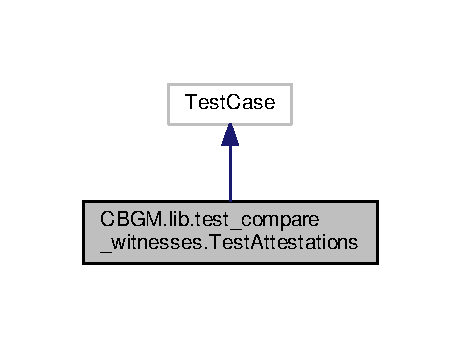
\includegraphics[width=221pt]{classCBGM_1_1lib_1_1test__compare__witnesses_1_1TestAttestations__inherit__graph}
\end{center}
\end{figure}


Collaboration diagram for C\+B\+G\+M.\+lib.\+test\+\_\+compare\+\_\+witnesses.\+Test\+Attestations\+:\nopagebreak
\begin{figure}[H]
\begin{center}
\leavevmode
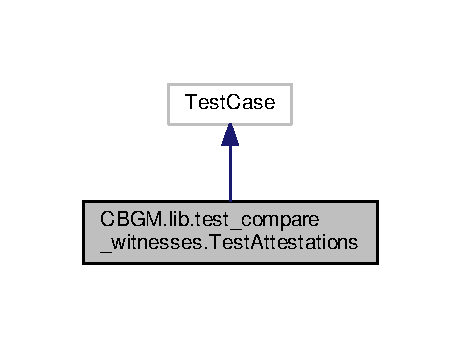
\includegraphics[width=221pt]{classCBGM_1_1lib_1_1test__compare__witnesses_1_1TestAttestations__coll__graph}
\end{center}
\end{figure}
\subsection*{Public Member Functions}
\begin{DoxyCompactItemize}
\item 
\mbox{\Hypertarget{classCBGM_1_1lib_1_1test__compare__witnesses_1_1TestAttestations_ad518e816fdd0e420c00cdbbc9d94e6d3}\label{classCBGM_1_1lib_1_1test__compare__witnesses_1_1TestAttestations_ad518e816fdd0e420c00cdbbc9d94e6d3}} 
def {\bfseries set\+Up\+Class} (cls)
\item 
\mbox{\Hypertarget{classCBGM_1_1lib_1_1test__compare__witnesses_1_1TestAttestations_a238f984e41a438393a5f9b02f40f4200}\label{classCBGM_1_1lib_1_1test__compare__witnesses_1_1TestAttestations_a238f984e41a438393a5f9b02f40f4200}} 
def {\bfseries tear\+Down\+Class} (cls)
\item 
\mbox{\Hypertarget{classCBGM_1_1lib_1_1test__compare__witnesses_1_1TestAttestations_a3d63670d257197883dafa8708f127841}\label{classCBGM_1_1lib_1_1test__compare__witnesses_1_1TestAttestations_a3d63670d257197883dafa8708f127841}} 
def {\bfseries test\+\_\+get\+\_\+attestations} (self)
\item 
\mbox{\Hypertarget{classCBGM_1_1lib_1_1test__compare__witnesses_1_1TestAttestations_a9538860a1f8fa09b217eb029334557f9}\label{classCBGM_1_1lib_1_1test__compare__witnesses_1_1TestAttestations_a9538860a1f8fa09b217eb029334557f9}} 
def {\bfseries test\+\_\+compare\+\_\+b\+\_\+c} (self)
\item 
\mbox{\Hypertarget{classCBGM_1_1lib_1_1test__compare__witnesses_1_1TestAttestations_a7562318a40e77c2e835e737413891af9}\label{classCBGM_1_1lib_1_1test__compare__witnesses_1_1TestAttestations_a7562318a40e77c2e835e737413891af9}} 
def {\bfseries test\+\_\+compare\+\_\+d\+\_\+e} (self)
\end{DoxyCompactItemize}
\subsection*{Public Attributes}
\begin{DoxyCompactItemize}
\item 
\mbox{\Hypertarget{classCBGM_1_1lib_1_1test__compare__witnesses_1_1TestAttestations_af4064021a4ba1bf7b5a102ef497dc9da}\label{classCBGM_1_1lib_1_1test__compare__witnesses_1_1TestAttestations_af4064021a4ba1bf7b5a102ef497dc9da}} 
{\bfseries test\+\_\+db}
\item 
\mbox{\Hypertarget{classCBGM_1_1lib_1_1test__compare__witnesses_1_1TestAttestations_a992ff2f94f8f3d679cdffe01b0938e5b}\label{classCBGM_1_1lib_1_1test__compare__witnesses_1_1TestAttestations_a992ff2f94f8f3d679cdffe01b0938e5b}} 
{\bfseries attestations}
\end{DoxyCompactItemize}


The documentation for this class was generated from the following file\+:\begin{DoxyCompactItemize}
\item 
lib/test\+\_\+compare\+\_\+witnesses.\+py\end{DoxyCompactItemize}

\hypertarget{classCBGM_1_1lib_1_1test__db_1_1TestDatabase}{}\section{C\+B\+G\+M.\+lib.\+test\+\_\+db.\+Test\+Database Class Reference}
\label{classCBGM_1_1lib_1_1test__db_1_1TestDatabase}\index{C\+B\+G\+M.\+lib.\+test\+\_\+db.\+Test\+Database@{C\+B\+G\+M.\+lib.\+test\+\_\+db.\+Test\+Database}}


Inheritance diagram for C\+B\+G\+M.\+lib.\+test\+\_\+db.\+Test\+Database\+:
\nopagebreak
\begin{figure}[H]
\begin{center}
\leavevmode
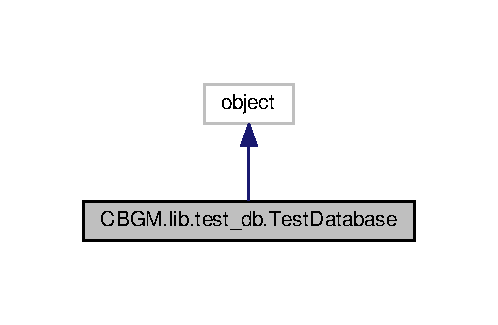
\includegraphics[width=239pt]{classCBGM_1_1lib_1_1test__db_1_1TestDatabase__inherit__graph}
\end{center}
\end{figure}


Collaboration diagram for C\+B\+G\+M.\+lib.\+test\+\_\+db.\+Test\+Database\+:
\nopagebreak
\begin{figure}[H]
\begin{center}
\leavevmode
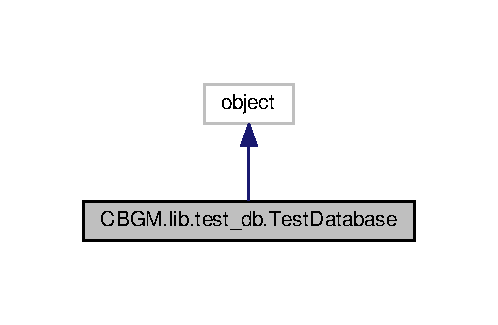
\includegraphics[width=239pt]{classCBGM_1_1lib_1_1test__db_1_1TestDatabase__coll__graph}
\end{center}
\end{figure}
\subsection*{Public Member Functions}
\begin{DoxyCompactItemize}
\item 
\mbox{\Hypertarget{classCBGM_1_1lib_1_1test__db_1_1TestDatabase_a5d9c034ab7f40291e3ec58a73fcbc8fe}\label{classCBGM_1_1lib_1_1test__db_1_1TestDatabase_a5d9c034ab7f40291e3ec58a73fcbc8fe}} 
def {\bfseries \+\_\+\+\_\+init\+\_\+\+\_\+} (self, data=I\+N\+P\+U\+T\+\_\+\+D\+A\+TA)
\item 
\mbox{\Hypertarget{classCBGM_1_1lib_1_1test__db_1_1TestDatabase_a28ea5e2bd5637fbc4fd5956045ffdb83}\label{classCBGM_1_1lib_1_1test__db_1_1TestDatabase_a28ea5e2bd5637fbc4fd5956045ffdb83}} 
def {\bfseries cleanup} (self)
\end{DoxyCompactItemize}
\subsection*{Public Attributes}
\begin{DoxyCompactItemize}
\item 
\mbox{\Hypertarget{classCBGM_1_1lib_1_1test__db_1_1TestDatabase_a567e6a237777c58b38b078b6019eac9e}\label{classCBGM_1_1lib_1_1test__db_1_1TestDatabase_a567e6a237777c58b38b078b6019eac9e}} 
{\bfseries py\+\_\+file}
\item 
\mbox{\Hypertarget{classCBGM_1_1lib_1_1test__db_1_1TestDatabase_a7c09c633b1487c49fab0bae4361622ec}\label{classCBGM_1_1lib_1_1test__db_1_1TestDatabase_a7c09c633b1487c49fab0bae4361622ec}} 
{\bfseries db\+\_\+file}
\end{DoxyCompactItemize}


The documentation for this class was generated from the following file\+:\begin{DoxyCompactItemize}
\item 
lib/test\+\_\+db.\+py\end{DoxyCompactItemize}

\hypertarget{classCBGM_1_1lib_1_1textual__flow_1_1TextualFlow}{}\section{C\+B\+G\+M.\+lib.\+textual\+\_\+flow.\+Textual\+Flow Class Reference}
\label{classCBGM_1_1lib_1_1textual__flow_1_1TextualFlow}\index{C\+B\+G\+M.\+lib.\+textual\+\_\+flow.\+Textual\+Flow@{C\+B\+G\+M.\+lib.\+textual\+\_\+flow.\+Textual\+Flow}}


Inheritance diagram for C\+B\+G\+M.\+lib.\+textual\+\_\+flow.\+Textual\+Flow\+:\nopagebreak
\begin{figure}[H]
\begin{center}
\leavevmode
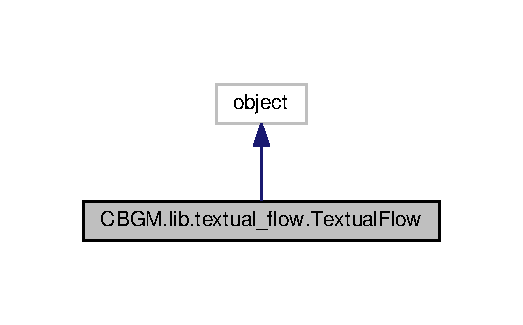
\includegraphics[width=251pt]{classCBGM_1_1lib_1_1textual__flow_1_1TextualFlow__inherit__graph}
\end{center}
\end{figure}


Collaboration diagram for C\+B\+G\+M.\+lib.\+textual\+\_\+flow.\+Textual\+Flow\+:\nopagebreak
\begin{figure}[H]
\begin{center}
\leavevmode
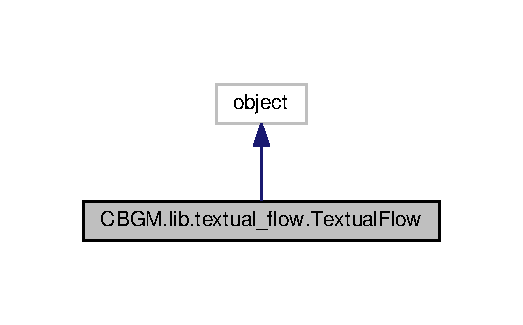
\includegraphics[width=251pt]{classCBGM_1_1lib_1_1textual__flow_1_1TextualFlow__coll__graph}
\end{center}
\end{figure}
\subsection*{Public Member Functions}
\begin{DoxyCompactItemize}
\item 
def \hyperlink{classCBGM_1_1lib_1_1textual__flow_1_1TextualFlow_ad70dfb8ec0a3602f6c9a5f962e8934e1}{\+\_\+\+\_\+init\+\_\+\+\_\+} (self, db\+\_\+file, variant\+\_\+unit, connectivity, perfect\+\_\+only=False, ranks\+\_\+on\+\_\+edges=True, include\+\_\+perc\+\_\+in\+\_\+label=True, show\+\_\+strengths=True, weak\+\_\+strength\+\_\+threshold=25, very\+\_\+weak\+\_\+strength\+\_\+threshold=5, show\+\_\+strength\+\_\+values=False, suffix=\textquotesingle{}\textquotesingle{}, box\+\_\+readings=False, min\+\_\+strength=None, include\+\_\+undirected=None, mpihandler=None)
\item 
def \hyperlink{classCBGM_1_1lib_1_1textual__flow_1_1TextualFlow_adc75c15bd885bfbd38c1a67c45acef88}{calculate\+\_\+textual\+\_\+flow} (self)
\item 
def \hyperlink{classCBGM_1_1lib_1_1textual__flow_1_1TextualFlow_af60312ac039b52328a2fca08923f4df8}{mpi\+\_\+result} (self, args, ret)
\end{DoxyCompactItemize}
\subsection*{Public Attributes}
\begin{DoxyCompactItemize}
\item 
\mbox{\Hypertarget{classCBGM_1_1lib_1_1textual__flow_1_1TextualFlow_aa972fedfb01abda3f42c5e87d18518a1}\label{classCBGM_1_1lib_1_1textual__flow_1_1TextualFlow_aa972fedfb01abda3f42c5e87d18518a1}} 
{\bfseries output\+\_\+files}
\item 
\mbox{\Hypertarget{classCBGM_1_1lib_1_1textual__flow_1_1TextualFlow_a3e178d015c4203f8009c58d9637e187b}\label{classCBGM_1_1lib_1_1textual__flow_1_1TextualFlow_a3e178d015c4203f8009c58d9637e187b}} 
{\bfseries connectivity}
\item 
\mbox{\Hypertarget{classCBGM_1_1lib_1_1textual__flow_1_1TextualFlow_a55d807ce601b82770a23fe5e4385e39e}\label{classCBGM_1_1lib_1_1textual__flow_1_1TextualFlow_a55d807ce601b82770a23fe5e4385e39e}} 
{\bfseries reading\+\_\+data}
\item 
\mbox{\Hypertarget{classCBGM_1_1lib_1_1textual__flow_1_1TextualFlow_ab0b6fc966f7802f523855516bd4acbec}\label{classCBGM_1_1lib_1_1textual__flow_1_1TextualFlow_ab0b6fc966f7802f523855516bd4acbec}} 
{\bfseries readings}
\item 
\mbox{\Hypertarget{classCBGM_1_1lib_1_1textual__flow_1_1TextualFlow_ac185378ca39fad5a8aae176afad372a8}\label{classCBGM_1_1lib_1_1textual__flow_1_1TextualFlow_ac185378ca39fad5a8aae176afad372a8}} 
{\bfseries mpihandler}
\item 
\mbox{\Hypertarget{classCBGM_1_1lib_1_1textual__flow_1_1TextualFlow_a089590ed65cf7c51e847243e29a5c72f}\label{classCBGM_1_1lib_1_1textual__flow_1_1TextualFlow_a089590ed65cf7c51e847243e29a5c72f}} 
{\bfseries db\+\_\+file}
\item 
\mbox{\Hypertarget{classCBGM_1_1lib_1_1textual__flow_1_1TextualFlow_aa6e67a465603bb34ea77c48e6eacdbb4}\label{classCBGM_1_1lib_1_1textual__flow_1_1TextualFlow_aa6e67a465603bb34ea77c48e6eacdbb4}} 
{\bfseries variant\+\_\+unit}
\item 
\mbox{\Hypertarget{classCBGM_1_1lib_1_1textual__flow_1_1TextualFlow_ace48f833a5c1058d7f9789a42e5e45a8}\label{classCBGM_1_1lib_1_1textual__flow_1_1TextualFlow_ace48f833a5c1058d7f9789a42e5e45a8}} 
{\bfseries perfect\+\_\+only}
\item 
\mbox{\Hypertarget{classCBGM_1_1lib_1_1textual__flow_1_1TextualFlow_aefc25a039ac1d85ec8d7abdf90a978aa}\label{classCBGM_1_1lib_1_1textual__flow_1_1TextualFlow_aefc25a039ac1d85ec8d7abdf90a978aa}} 
{\bfseries ranks\+\_\+on\+\_\+edges}
\item 
\mbox{\Hypertarget{classCBGM_1_1lib_1_1textual__flow_1_1TextualFlow_a93604cde7ea6620173270a6d3c10c195}\label{classCBGM_1_1lib_1_1textual__flow_1_1TextualFlow_a93604cde7ea6620173270a6d3c10c195}} 
{\bfseries include\+\_\+perc\+\_\+in\+\_\+label}
\item 
\mbox{\Hypertarget{classCBGM_1_1lib_1_1textual__flow_1_1TextualFlow_a5a89d996be59a383c2e075ee83c288e9}\label{classCBGM_1_1lib_1_1textual__flow_1_1TextualFlow_a5a89d996be59a383c2e075ee83c288e9}} 
{\bfseries show\+\_\+strengths}
\item 
\mbox{\Hypertarget{classCBGM_1_1lib_1_1textual__flow_1_1TextualFlow_a37b4c7d01884812da946204c18c2e93d}\label{classCBGM_1_1lib_1_1textual__flow_1_1TextualFlow_a37b4c7d01884812da946204c18c2e93d}} 
{\bfseries weak\+\_\+strength\+\_\+threshold}
\item 
\mbox{\Hypertarget{classCBGM_1_1lib_1_1textual__flow_1_1TextualFlow_a7100ba33750972d292325f0cfa02d773}\label{classCBGM_1_1lib_1_1textual__flow_1_1TextualFlow_a7100ba33750972d292325f0cfa02d773}} 
{\bfseries very\+\_\+weak\+\_\+strength\+\_\+threshold}
\item 
\mbox{\Hypertarget{classCBGM_1_1lib_1_1textual__flow_1_1TextualFlow_ab978865dbc49de9740cc073c6b3cf7ec}\label{classCBGM_1_1lib_1_1textual__flow_1_1TextualFlow_ab978865dbc49de9740cc073c6b3cf7ec}} 
{\bfseries show\+\_\+strength\+\_\+values}
\item 
\mbox{\Hypertarget{classCBGM_1_1lib_1_1textual__flow_1_1TextualFlow_a6c43872f5693e2796804a65cfa9ff67f}\label{classCBGM_1_1lib_1_1textual__flow_1_1TextualFlow_a6c43872f5693e2796804a65cfa9ff67f}} 
{\bfseries suffix}
\item 
\mbox{\Hypertarget{classCBGM_1_1lib_1_1textual__flow_1_1TextualFlow_aa18db9753a0c2a6bac690b88a60e8d78}\label{classCBGM_1_1lib_1_1textual__flow_1_1TextualFlow_aa18db9753a0c2a6bac690b88a60e8d78}} 
{\bfseries box\+\_\+readings}
\item 
\mbox{\Hypertarget{classCBGM_1_1lib_1_1textual__flow_1_1TextualFlow_a648c7aa34e9a79385c0b3c405030f7a5}\label{classCBGM_1_1lib_1_1textual__flow_1_1TextualFlow_a648c7aa34e9a79385c0b3c405030f7a5}} 
{\bfseries parent\+\_\+maps}
\item 
\mbox{\Hypertarget{classCBGM_1_1lib_1_1textual__flow_1_1TextualFlow_a200d89d1d15cf1ac7484de22fa5f12d6}\label{classCBGM_1_1lib_1_1textual__flow_1_1TextualFlow_a200d89d1d15cf1ac7484de22fa5f12d6}} 
{\bfseries min\+\_\+strength}
\item 
\mbox{\Hypertarget{classCBGM_1_1lib_1_1textual__flow_1_1TextualFlow_aec9ec697f19a6a2ef3a6396ecbb89412}\label{classCBGM_1_1lib_1_1textual__flow_1_1TextualFlow_aec9ec697f19a6a2ef3a6396ecbb89412}} 
{\bfseries include\+\_\+undirected}
\end{DoxyCompactItemize}


\subsection{Constructor \& Destructor Documentation}
\mbox{\Hypertarget{classCBGM_1_1lib_1_1textual__flow_1_1TextualFlow_ad70dfb8ec0a3602f6c9a5f962e8934e1}\label{classCBGM_1_1lib_1_1textual__flow_1_1TextualFlow_ad70dfb8ec0a3602f6c9a5f962e8934e1}} 
\index{C\+B\+G\+M\+::lib\+::textual\+\_\+flow\+::\+Textual\+Flow@{C\+B\+G\+M\+::lib\+::textual\+\_\+flow\+::\+Textual\+Flow}!\+\_\+\+\_\+init\+\_\+\+\_\+@{\+\_\+\+\_\+init\+\_\+\+\_\+}}
\index{\+\_\+\+\_\+init\+\_\+\+\_\+@{\+\_\+\+\_\+init\+\_\+\+\_\+}!C\+B\+G\+M\+::lib\+::textual\+\_\+flow\+::\+Textual\+Flow@{C\+B\+G\+M\+::lib\+::textual\+\_\+flow\+::\+Textual\+Flow}}
\subsubsection{\texorpdfstring{\+\_\+\+\_\+init\+\_\+\+\_\+()}{\_\_init\_\_()}}
{\footnotesize\ttfamily def C\+B\+G\+M.\+lib.\+textual\+\_\+flow.\+Textual\+Flow.\+\_\+\+\_\+init\+\_\+\+\_\+ (\begin{DoxyParamCaption}\item[{}]{self,  }\item[{}]{db\+\_\+file,  }\item[{}]{variant\+\_\+unit,  }\item[{}]{connectivity,  }\item[{}]{perfect\+\_\+only = {\ttfamily False},  }\item[{}]{ranks\+\_\+on\+\_\+edges = {\ttfamily True},  }\item[{}]{include\+\_\+perc\+\_\+in\+\_\+label = {\ttfamily True},  }\item[{}]{show\+\_\+strengths = {\ttfamily True},  }\item[{}]{weak\+\_\+strength\+\_\+threshold = {\ttfamily 25},  }\item[{}]{very\+\_\+weak\+\_\+strength\+\_\+threshold = {\ttfamily 5},  }\item[{}]{show\+\_\+strength\+\_\+values = {\ttfamily False},  }\item[{}]{suffix = {\ttfamily \textquotesingle{}\textquotesingle{}},  }\item[{}]{box\+\_\+readings = {\ttfamily False},  }\item[{}]{min\+\_\+strength = {\ttfamily None},  }\item[{}]{include\+\_\+undirected = {\ttfamily None},  }\item[{}]{mpihandler = {\ttfamily None} }\end{DoxyParamCaption})}

\begin{DoxyVerb}@param db_file: sqlite database
@param variant_unit: draw the textual flow of this variant unit
@param connectivity: maximum allowable rank of parents
@param perfect_only: raise an exception if coherence is not perfect (I.e. this is a forest)
@param ranks_on_edges: label the ranks on the edges rather than in the nodes
@param include_perc_in_label: show the coherence percentage of a parent in the label (edges only)
@param show_strengths: show the strength of textual flow as width of edges
@param weak_strength_threshold: strength weaker than this will be shown as "weak"
@param very_weak_strength_threshold: strength weaker than this will be shown as "very weak"
@param show_strength_values: show the prior/posterior values under the edge label
@param suffix: suffix to use in filename (before the extension)
@param box_readings: Draw a diagram for each reading in a box
@param min_strength: Minimum strength for genealogical coherence relationships (default None = disabled)
@param include_undirected: Include undirected relationships (as a group)
@param mpihandler: optional MpiHandler instance
\end{DoxyVerb}
 

\subsection{Member Function Documentation}
\mbox{\Hypertarget{classCBGM_1_1lib_1_1textual__flow_1_1TextualFlow_adc75c15bd885bfbd38c1a67c45acef88}\label{classCBGM_1_1lib_1_1textual__flow_1_1TextualFlow_adc75c15bd885bfbd38c1a67c45acef88}} 
\index{C\+B\+G\+M\+::lib\+::textual\+\_\+flow\+::\+Textual\+Flow@{C\+B\+G\+M\+::lib\+::textual\+\_\+flow\+::\+Textual\+Flow}!calculate\+\_\+textual\+\_\+flow@{calculate\+\_\+textual\+\_\+flow}}
\index{calculate\+\_\+textual\+\_\+flow@{calculate\+\_\+textual\+\_\+flow}!C\+B\+G\+M\+::lib\+::textual\+\_\+flow\+::\+Textual\+Flow@{C\+B\+G\+M\+::lib\+::textual\+\_\+flow\+::\+Textual\+Flow}}
\subsubsection{\texorpdfstring{calculate\+\_\+textual\+\_\+flow()}{calculate\_textual\_flow()}}
{\footnotesize\ttfamily def C\+B\+G\+M.\+lib.\+textual\+\_\+flow.\+Textual\+Flow.\+calculate\+\_\+textual\+\_\+flow (\begin{DoxyParamCaption}\item[{}]{self }\end{DoxyParamCaption})}

\begin{DoxyVerb}Create textual flow diagram(s) for the specified variant unit.

Because I put the whole textual flow in one diagram (unlike Munster who
show a textual flow diagram for a single reading) there can be multiple
ancestors for a witness...
\end{DoxyVerb}
 \mbox{\Hypertarget{classCBGM_1_1lib_1_1textual__flow_1_1TextualFlow_af60312ac039b52328a2fca08923f4df8}\label{classCBGM_1_1lib_1_1textual__flow_1_1TextualFlow_af60312ac039b52328a2fca08923f4df8}} 
\index{C\+B\+G\+M\+::lib\+::textual\+\_\+flow\+::\+Textual\+Flow@{C\+B\+G\+M\+::lib\+::textual\+\_\+flow\+::\+Textual\+Flow}!mpi\+\_\+result@{mpi\+\_\+result}}
\index{mpi\+\_\+result@{mpi\+\_\+result}!C\+B\+G\+M\+::lib\+::textual\+\_\+flow\+::\+Textual\+Flow@{C\+B\+G\+M\+::lib\+::textual\+\_\+flow\+::\+Textual\+Flow}}
\subsubsection{\texorpdfstring{mpi\+\_\+result()}{mpi\_result()}}
{\footnotesize\ttfamily def C\+B\+G\+M.\+lib.\+textual\+\_\+flow.\+Textual\+Flow.\+mpi\+\_\+result (\begin{DoxyParamCaption}\item[{}]{self,  }\item[{}]{args,  }\item[{}]{ret }\end{DoxyParamCaption})}

\begin{DoxyVerb}Handle an MPI result
@param args: original args sent to get_parents
@param ret: response from the child
\end{DoxyVerb}
 

The documentation for this class was generated from the following file\+:\begin{DoxyCompactItemize}
\item 
lib/textual\+\_\+flow.\+py\end{DoxyCompactItemize}

\hypertarget{classCBGM_1_1lib_1_1genealogical__coherence_1_1TooManyAborts}{}\section{C\+B\+G\+M.\+lib.\+genealogical\+\_\+coherence.\+Too\+Many\+Aborts Class Reference}
\label{classCBGM_1_1lib_1_1genealogical__coherence_1_1TooManyAborts}\index{C\+B\+G\+M.\+lib.\+genealogical\+\_\+coherence.\+Too\+Many\+Aborts@{C\+B\+G\+M.\+lib.\+genealogical\+\_\+coherence.\+Too\+Many\+Aborts}}


Inheritance diagram for C\+B\+G\+M.\+lib.\+genealogical\+\_\+coherence.\+Too\+Many\+Aborts\+:\nopagebreak
\begin{figure}[H]
\begin{center}
\leavevmode
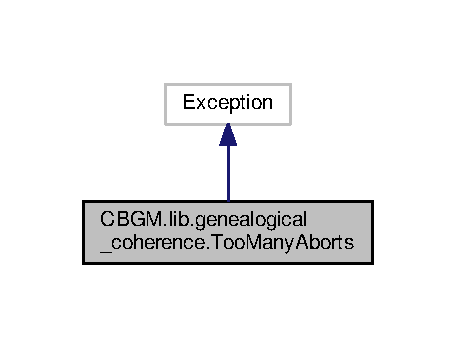
\includegraphics[width=219pt]{classCBGM_1_1lib_1_1genealogical__coherence_1_1TooManyAborts__inherit__graph}
\end{center}
\end{figure}


Collaboration diagram for C\+B\+G\+M.\+lib.\+genealogical\+\_\+coherence.\+Too\+Many\+Aborts\+:\nopagebreak
\begin{figure}[H]
\begin{center}
\leavevmode
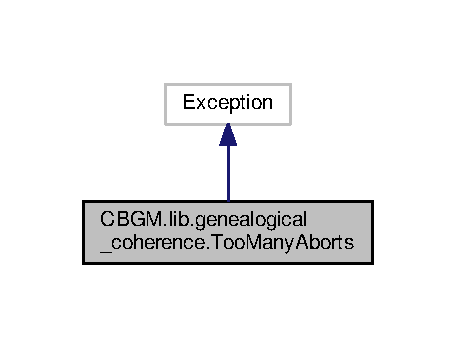
\includegraphics[width=219pt]{classCBGM_1_1lib_1_1genealogical__coherence_1_1TooManyAborts__coll__graph}
\end{center}
\end{figure}


The documentation for this class was generated from the following file\+:\begin{DoxyCompactItemize}
\item 
lib/genealogical\+\_\+coherence.\+py\end{DoxyCompactItemize}

%--- End generated contents ---

% Index
\backmatter
\newpage
\phantomsection
\clearemptydoublepage
\addcontentsline{toc}{chapter}{Index}
\printindex

\end{document}
